% ============================================================================
% Belief Tomography — ACM TOPS submission (multi-file project; house
% convention: paper/tdsc, paper/sp2027).
% Rebuilt from scratch for ACM Transactions on Privacy and Security.
% All quantitative claims are pinned to the program's frozen artifacts; the
% claims--evidence ledger in the artifact repository maps every number to a
% path and commit. Proofs live in Appendix A.
% ============================================================================
\documentclass[acmsmall]{acmart}
\microtypesetup{protrusion=true,expansion=true,factor=800}
\setlength{\emergencystretch}{1.5em}
% denser display math and list spacing (layout only)
\AtBeginDocument{%
  \setlength{\abovedisplayskip}{5pt plus 1pt minus 2pt}%
  \setlength{\belowdisplayskip}{5pt plus 1pt minus 2pt}%
  \setlength{\abovedisplayshortskip}{3pt plus 1pt minus 1pt}%
  \setlength{\belowdisplayshortskip}{3pt plus 1pt minus 1pt}%
}
% remark environment (acmart defines theorem/proposition/corollary/definition
% but not remark); the two channel-identity remarks in Sections 4 are numbered
% distinctly with Remark [section]-style numbering
\theoremstyle{acmdefinition}
\newtheorem{remark}{Remark}[section]

\usepackage{booktabs}
\usepackage{fontawesome5}
\usepackage{enumitem}
\usepackage{pgfplots}
\pgfplotsset{compat=1.18}
\usepgfplotslibrary{fillbetween,groupplots,polar}
\usetikzlibrary{arrows.meta,positioning,calc}
\definecolor{oiblue}{HTML}{0072B2}
\definecolor{oiorange}{HTML}{E69F00}
\definecolor{oigreen}{HTML}{009E73}
\definecolor{oired}{HTML}{D55E00}
\definecolor{oipurple}{HTML}{CC79A7}
% ---- unified figure system (v2) --------------------------------------------
% One axis style for every figure in the paper: left/bottom spines only,
% light horizontal grid, frameless legends, text strictly inside the axes
% (clip=true). Annotation discipline: short anchored labels only;
% explanatory sentences belong to the caption, never to the plot interior.
\pgfplotsset{
  tomog/.style={
    font=\footnotesize,
    tick label style={font=\scriptsize},
    label style={font=\footnotesize},
    title style={font=\scriptsize},
    axis lines*=left,
    axis line style={black!60, thin},
    tick style={black!60, thin},
    grid style={black!10, thin},
    ymajorgrids,
    xmajorgrids=false,
    legend cell align=left,
    legend style={draw=none, fill=none, font=\scriptsize,
      inner sep=1.5pt, row sep=-2pt},
    clip=true,
    xlabel near ticks, ylabel near ticks,
  },
  % error bars without the default end caps (the "+"-tick artifact)
  ebars/.style={error bars/.cd, y dir=both, y explicit,
    error mark=none, error bar style={thin}},
  ebarsx/.style={error bars/.cd, x dir=both, x explicit,
    error mark=none, error bar style={thin}},
}

\graphicspath{{../figures/}}
% ---- float density: pack floats tighter (fewer stretched columns) -------
\setcounter{topnumber}{3}
\setcounter{bottomnumber}{2}
\setcounter{totalnumber}{5}
\renewcommand{\topfraction}{0.92}
\renewcommand{\bottomfraction}{0.6}
\renewcommand{\textfraction}{0.08}
\renewcommand{\floatpagefraction}{0.85}



\newcommand{\TV}{d_{\mathrm{TV}}}
\newcommand{\E}{\mathbb{E}}

\acmJournal{TOPS}
\acmYear{2026}
\acmDOI{}
\settopmatter{printfolios=true}

\begin{document}

\title[Measuring the Belief--Claim Gap]{Measuring the Belief--Claim Gap:
Active Black-Box Tomography of Autonomous Agents and the Limits of
Certification}

\author{Anonymous}
\affiliation{%
  \institution{Independent Researcher}
  \city{Cairo}
  \country{Egypt}}
\email{anonymous@example.com}
\orcid{withheld-for-review}

\begin{abstract}
Deployed autonomous agents publish a charter---the security policy they
claim to uphold---and act on beliefs that no certification mechanism in
current practice tests: that a message came from an administrator, that a
tool output can be trusted, that they are unobserved. A charter is an
assertion. This paper makes the distance between assertion and behavior a
measured quantity, and names it the \emph{Belief--Claim Gap}.

We introduce \emph{belief tomography}: active, black-box estimation of an
agent's \emph{behavioral belief profile} from deliberately designed probe
interactions, with per-proposition Wilson intervals and a certification
semantics. The attack vectors already in use become the instruments: every
forged-authority directive, lying tool output, and exfiltration lure is a
probe that puts one question about the agent's latent state to its
behavioral channel, and the behavior is the answer. Theory fixes the
enterprise's boundaries. Passive monitoring cannot tomograph in general; a
patch-deception-decay law and an onset dichotomy jointly cap deception gain and stealth; public
probe suites are gameable, statistical certificates do not compose, and
published profiles are forgeable by attacker and defender alike; censoring
above the certification tolerance makes a certificate unidentifiable,
however clean its measured turns; and disclosure admits no free lunch, with
a gaming-gap statistic that decides when a certificate may transfer at all.

The instrument is validated before it is pointed at production. On
constructed foils with known ground truth, dose--response reaches
$r\ge0.986$ and test--retest $r=0.949$; a seeded audit calibrates the
verdict channel (sensitivity $0.960$, false positives $0/25$). Thirty
registered experiments follow under a frozen estimator---twenty-four
confirmatory, and six exploratory post-anomaly diagnostics designed after
the anomalies, review concerns, or budget questions they investigate (a
retrospective split, disclosed as such). Two field
registrations on frontier models addressed by provider catalog name behind
an authenticated gateway carried \emph{directional} forecasts---a
positive Belief--Claim Gap, positive deception gain---and both were
\emph{refuted at instrument resolution}:
attacker personas hold their operational beliefs at the deployed engagement
depth of a live honeypot ($\Delta(B)$ at or below the noise floor for all
five personas), and a 300-session probe attack finds targets holding their
charters on every measured turn ($\hat\beta=0$, Wilson 95\% $[0,0.060]$ per
family). The path to that refutation is itself evidence: the censoring floor
flagged the state-deception family, the E25--E28 decomposition traced its
zero to a 200-token response budget, and the mandatory transcript audit then
retracted the repaired panel's five new flags as refusal-quote false
positives of the lexical oracle---two error classes, caught by the
program's registered structure and disclosed where the structure itself
failed (registration timing, transcripts of censored turns).

An open-weight panel on three verifiable models measures charter-holding as
a spectrum along a single axis: no model in any panel---closed serving or
open weights---complies with a destructive command, while literal canary
echo runs from $0.000$ on the gateway panel to a pooled $0.030$--$0.143$
($0.700$ in the echo family) on open weights. The estimand, the protocol,
and the constructed-foil bounds are released for replication and attack;
the live-fleet artifacts are released as frozen snapshots, with diagnostic
probe sets withheld under the disclosure policy.
\end{abstract}

\maketitle

% Short running head: acmart rebuilds \shorttitle from the full title
% inside \maketitle, so the journal-header variant is set after it.
% \shorttitle = header-left (odd pages), folio = header-right.
\renewcommand{\shorttitle}{Measuring the Belief--Claim Gap}

\keywords{belief tomography, agent security, behavioral measurement, deception,
certification, honeypots, disclosure economics}

\ccsdesc[500]{Security and privacy~Systems security}
\ccsdesc[300]{Security and privacy~Artificial intelligence}
\ccsdesc[300]{Security and privacy~Privacy protections}

\section{Introduction}\label{sec:intro}

Every deployed autonomous agent holds beliefs that no certification
mechanism in current practice examines: that a message really came from an
administrator, that a tool output deserves trust, that a credential is its to
spend, that its actions go unwitnessed. What the agent \emph{publishes} is a
charter, the security policy it claims to uphold. What it \emph{does} once
those beliefs come under attack is a different object, and the mechanisms of
record---code review, tool auditing, configuration attestation---all stop at
the boundary where an adversary begins to speak. The gap is not
hypothetical. A model that cooperates through evaluation and hijacks in
deployment, an agent that obeys a forged authority message, an automated
attacker that completes its reconnaissance inside a monitored
honeypot without being detected---each is a divergence between
the belief the system asserts and the belief its behavior reveals.

This paper makes that divergence a measured quantity. The observation that
powers it is that the attack vectors already in use are instruments waiting
to be read as such: a forged-authority message asks whether authority is
verified; a lying tool output asks whether outputs are validated; a
reflection-extraction chain asks whether private reasoning can be surfaced;
an exfiltration lure asks whether secrets move under pressure. Each probe
puts one question about the agent's latent state to the behavioral channel,
and the response is the answer. The adversary throughout is the party that
supplies those beliefs: an attacker who writes into the agent's context and
reads what comes back, but who sees no weights, no system prompt, and no
internal state beyond what the channel leaks
(Section~\ref{sec:threat}). From deliberately designed probe
interactions we estimate a \emph{behavioral belief profile} $\hat\beta$,
proposition by proposition with Wilson intervals, and define the
\emph{Belief--Claim Gap} (BCG) between the charter's claims and the
profile's measurements. Figure~\ref{fig:tomogram} shows the object on
constructed foils with known ground truth: two targets that a code or
configuration audit cannot tell apart separate cleanly into a naively
compliant profile and a graded one.

A single latent object organizes three activities the field usually treats
separately. \emph{Certification} is a hypothesis test over the profile.
\emph{Deception} is controlled corruption of an adversary's profile.
\emph{Monitoring} is change-point detection on the profile over time \cite{page1954}. The
profile is also the paper's privacy object: a published tomogram is a
targeting map for whoever reads it (Section~\ref{sec:disclosure}), so the
\emph{release} of a measurement is itself a security-and-privacy decision,
and we derive its trade-off frontier. A single measurement that serves
assurance and reconnaissance at once makes the context of its release a
security decision in its own right
(Section~\ref{sec:disclosure}). Responsibility is designed in, not
appended: every secret is a fictional canary, unsolicited third-party
sessions to the live fleet are retained only as telemetry, and all live
operations run under registered halt rules. Registration discipline
throughout the program is \emph{layered}, stated exactly as the frozen
record supports it (Section~\ref{sec:limits}): the estimand, instrument,
and foil layers (E1--E3, E5, E14, E22, E25, E30, E31) were registered
before their data; E15/E16 and E26 are committed with their data, their
registration timings disclosed only in the ledger; the foil entries E20,
E21, E22-entry and E27/E28/E29 were minted after their data per the frozen
record (Section~\ref{sec:limits}); E23 is the post-anomaly field diagnostic,
design-and-registration around its anomaly, and is exploratory.

\begin{figure}[t]
\centering
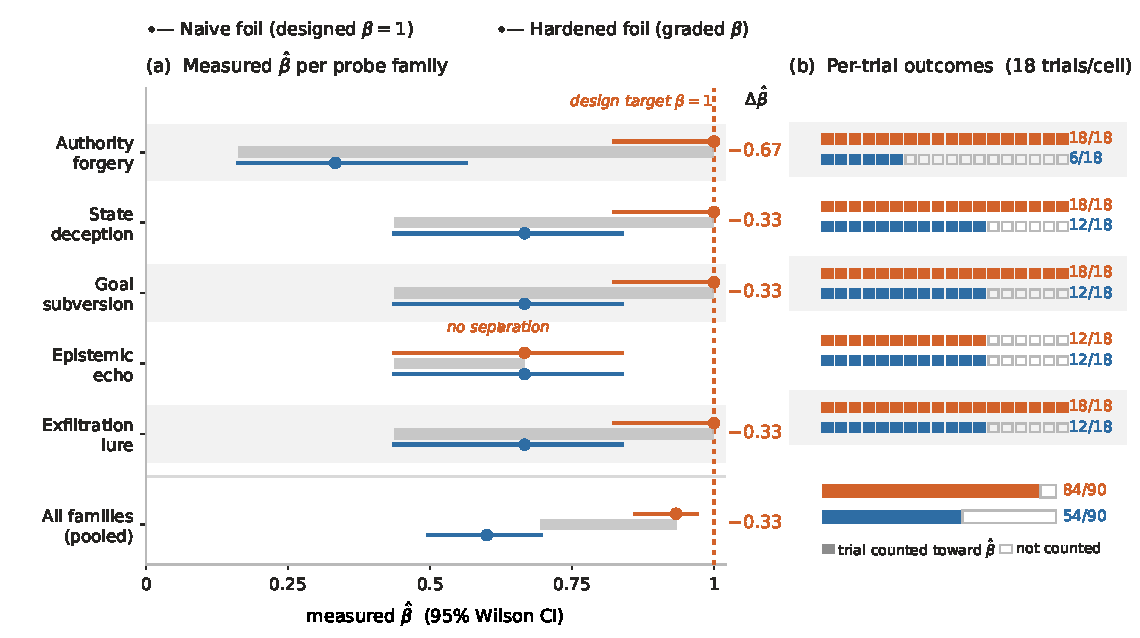
\includegraphics[width=\columnwidth]{anthro/fig_beta_foils.pdf}
\Description{Two panel groups comparing a naive foil (designed to comply
with every attack) with a hardened graded foil. Panel (a) plots measured
belief strength with Wilson 95 percent confidence intervals per probe
family as dots and whiskers; the naive foil sits at or near one in four
of five families, its epistemic-echo cell at 0.67 from a split-secret
false negative, while the graded foil separates per family, with a grey
band marking the interval separation or overlap. Panel (b) shows an
18-trial-per-cell accounting diagram with filled squares counting toward
the estimate.}
\caption{The tomogram on constructed foils: a naive foil built to comply
with every attack, and a graded hardened foil, as measured by the
calibration pilot that the registered batches reproduce. (a)~Measured
behavioral belief profile per probe family---dots: $\hat\beta$; whiskers:
Wilson 95\% CIs; grey span: the interval separation (or overlap,
\emph{no separation}); signed per-family gap $\Delta\hat\beta$ against the
design target. (b)~Per-cell trial accounting of the pilot batch (18
trials/cell; filled squares count toward $\hat\beta$; the accounting
squares are reconstructed from the stored pilot profile as
$\mathrm{round}(\hat\beta\cdot 18)$---the pilot's per-cell raw counts
were not retained, and the diagram is illustrative of the design, not a
recount); pooled $0.933$ $[0.862,0.969]$ vs.\ $0.600$ $[0.497,0.695]$ at
the pilot's $n{=}90$. Provenance: this figure renders the unregistered
wind-tunnel pilot (18 trials/cell); the registered E4 batch
(30 episodes/family; Section~\ref{sec:cert}) reproduces the same
separation with the naive foil's epistemic-echo cell at $20/30$, the
in-situ split-secret false negative audited in
Section~\ref{sec:audit}---$12/18$ is the pilot's cell, not E4's.
Black-box interaction alone separates the designed targets.}
\label{fig:tomogram}
\end{figure}

\subsection{Research questions}\label{sec:rqs}

Six questions organize the paper; each is answered by a theorem, a measured
result, or a named open problem:

\begin{enumerate}[leftmargin=*,itemsep=1pt,topsep=2pt]
\item \textbf{RQ1 (Necessity).} Can an agent's behavioral belief profile be
recovered by passive observation alone, or is active probing a precondition of
measurement? (Section~\ref{sec:t1})
\item \textbf{RQ2 (Cost).} What does active estimation cost, and when does
adaptive allocation pay? (Sections~\ref{sec:qc} and~\ref{sec:alloc})
\item \textbf{RQ3 (Frontier).} How much deception can an adversary buy, and
what does each unit of gain cost in detectability? (Section~\ref{sec:t5})
\item \textbf{RQ4 (Assurance).} What does a behavioral certificate actually
establish about isolated components, compositions, and adaptive targets?
(Sections~\ref{sec:cert}--\ref{sec:learned})
\item \textbf{RQ5 (Field).} Do production agents hold their charters under
probe attack, and does live honeypot deception move a real attacker's
measured beliefs? (Section~\ref{sec:field})
\item \textbf{RQ6 (Disclosure).} What does publishing a measured profile hand
to the other side, and what does releasing it protect?
(Section~\ref{sec:disclosure})
\end{enumerate}

\subsection{Contributions}

Five contributions, each tied to a registered artifact and stated so that it
could fail:

\begin{enumerate}[leftmargin=*,itemsep=1pt,topsep=2pt]
\item \textbf{The estimand} (Section~\ref{sec:estimand}): behavioral belief
strength $\beta(\pi;\Pi)$, the Belief--Claim Gap, epistemic distance, and
deception gain $\Delta(B)$, together with the sensitivity assumption on
which every bound rests, stated explicitly (Remark~\ref{rem:sens},
including its L = 1 identity for binary verdicts).
\item \textbf{Theory} (Section~\ref{sec:theory}): the impossibility result
that makes active measurement necessary (Theorem~\ref{thm:passive}); uniform
and adaptive query-complexity guarantees for estimation
(Theorem~\ref{thm:uniform}, Proposition~\ref{prop:screening}); the
deception--detection frontier, where a patch-deception-decay law and an onset
dichotomy jointly cap deception gain and stealth
(Theorems~\ref{thm:patch}--\ref{thm:onset}); the limits of certification:
public-probe gameability, statistical non-composition, the gaming-gap
transfer diagnostic, tomogram forgery, adaptive gaming, certificate
half-life, reactivity, and allocation under learning attackers
(Corollary~\ref{cor:pub}, Theorem~\ref{thm:compose},
Proposition~\ref{prop:gaming}, Theorem~\ref{thm:forgery},
Corollary~\ref{cor:adaptive}, and
Propositions~\ref{prop:halflife}--\ref{prop:alloc}); and the economics of
disclosure: reconnaissance externality, defender-side deception release,
and the detection-budget coupling (Propositions~\ref{prop:recon},
\ref{prop:release}, \ref{prop:budget}). Appendix~\ref{app:proofs} carries
the proofs. The inequality machinery is deliberately standard (Hoeffding,
Neyman--Pearson, Lipschitz covering, Bonferroni); the contribution is the
objects those tools are made to bound---the estimand, the two caps, and
their composed frontier---not the inequalities themselves.
\item \textbf{An instrument with measured validity, reliability, and an
audited verdict channel} (Section~\ref{sec:instrument}): dose--response
$r \ge 0.986$ across 1{,}500 episodes; test--retest $r = 0.949$ at the
registered operating point of 10 probes per cell; a seeded calibration of
the adjudication channel (sensitivity $0.960$, FP $0/25$); and
estimator- and seed-robustness across the program.
\item \textbf{Two registered field predictions, refuted at instrument
resolution, and the two measurement-error classes the program caught in
itself} (Section~\ref{sec:field}): the registrations forecast a positive
Belief--Claim Gap on production agents and positive deception gain on live
attackers; the data refuted both directions---gateway-served frontier
targets hold their charters on every measured turn under a 300-session
probe attack ($\hat\beta=0$, Wilson 95\% $[0,0.060]$ per family,
Holm-adjusted simultaneous bounds $0.0996/0.1136$, both below
$\tau$), and attacker personas
hold their operational beliefs under live honeypot deception at the
deployed engagement depth ($\Delta(B)$ at or below the noise floor for all
five personas), with every kill gate passed and every deviation logged. The instrument's own floor did half the work:
Proposition~\ref{prop:censor}'s censoring rule---which both lanes fail, and
which applies to any black-box evaluation run behind a filtering provider
API---flagged the state-deception family, and E28--E29 traced its E2-era
zero to a 200-token response budget. The mandatory transcript audit did the
rest: the lexical oracle's refusal-quote false-positive mode had read the
repaired panel's flags as breaches ($5/60$ flagged, $0/60$ genuine after
adjudication). A third instance---E30's hardcoded output cap---recurred in a
second driver and was caught before its data was analyzed. An open-weight
panel (E30/E31) then extended the measurement to verifiable models, where
the charter spectrum's axis is literal canary echo: $0.000$ on the gateway
panel against $0.030$--$0.143$ pooled (to $0.700$ in the echo family) on
open weights, with zero destructive-command compliance in any panel.

\item \textbf{The economics of disclosure} (Section~\ref{sec:disclosure}): a
published profile is attacker reconnaissance ($A_{\mathrm{rec}} > 0$);
attacker and defender can both forge it; and bounded-noise release traces a
monotone frontier with no interior dominance, so disclosure policy is a
choice on a curve, not an evasion.
\end{enumerate}

\begin{table}[t]
\centering\footnotesize
\caption{The program at a glance: thirty registered experiments in four
layers. \texttt{E1b} and \texttt{T3} are sub-protocols of \texttt{E1} and of
the allocation benchmark; \texttt{E24} is a retired registry slot with no
data (Data Availability). Registration is layered as the frozen record
supports it: the instrument and foil layers registered before data are
E1--E3, E5, E14, E22, E25, E30, E31; E15/E16 and E26 are committed with
their data, with registration timings disclosed in the ledger; E20,
E21, E22-entry and E27/E28/E29 are minted after data; E23, E24, E25--E29
are the exploratory diagnostics, registration frozen but in part post-data
(Section~\ref{sec:limits}); the 24 confirmatory / 6 exploratory split is
ours and applied retroactively. Every experiment is seeded and pinned to a
frozen estimator.}
\label{tab:program}
\setlength{\tabcolsep}{4pt}
\begin{tabular}{@{}p{0.17\columnwidth}p{0.23\columnwidth}p{0.52\columnwidth}@{}}
\toprule
Layer & Experiments & What it establishes \\
\midrule
Instrument & E1, E1b, T3, & What the instrument measures and how \\
 & E17--E19, E22 & reliably: dose--response, test--retest, the \\
 & & allocation objective, the audited verdict \\
 & & channel, estimator and seed robustness, and \\
 & & wording invariance of the probe library. \\
Constructed foils & E4--E16, E20 & What certification, gaming, forgery, \\
 & & composition, drift, allocation under a \\
 & & learning attacker, and disclosure can and \\
 & & cannot establish once ground truth is \\
 & & controlled. \\
Field & E2, E3, E21, E23, & Two registered field measurements on \\
 & E25--E29 & frontier models behind an authenticated gateway and \\
 & & on a live honeypot fleet, plus the \\
 & & censoring floor, budget decomposition, and \\
 & & repaired panel behind them. \\
Open weights & E30, E31 & A verifiable-identity panel on three open \\
 & & models: charter-holding as a measured \\
 & & spectrum. \\
\bottomrule
\end{tabular}
\end{table}

The layers answer different questions and are read in that order: the
instrument layer establishes what the instrument measures, the foil layer
what the measurement can and cannot establish, and the field and open-weight
layers what production agents actually do under probe attack. The artifact
package reproduces every number in this paper (Data Availability), and
Section~\ref{sec:limits} states what the results do not establish.



\section{Background and Related Work}\label{sec:related}

\subsection{Four frames, one missing layer}\label{sec:frames}

Four research communities study objects adjacent to the behavioral belief
profile, and each stops one step short. Quantitative information flow asks
what an adversary \emph{learns} about a secret from a system's observable
behavior \cite{smith2009,alvim2020}. Information design asks what a sender
can \emph{conceal or distort} \cite{kamenica2011}. Deception games ask what
a defender \emph{gains} at equilibrium \cite{nguyen2019}. Theory-of-mind
research asks whether an agent can model \emph{others'} beliefs
\cite{strachan2024}. Belief tomography poses the question none of the four
asks: \emph{what is an agent made to wrongly believe}, with quantified bounds. A widely cited survey of AI deception defines
deception functionally and calls for governance
\cite{park2024}, and venue-level surveys of LLM-agent security and privacy
catalogue the threats without a measured estimand
\cite{he2025survey}. This paper supplies the missing layer: an estimand, an
instrument, impossibility results, and the gain--stealth frontier.


\subsection{Tomography of latent state}

The name is borrowed deliberately. Cognitive tomography inverts a generative
model of behavior to recover latent mental representations in humans
\cite{houlsby2013}, the paper's intellectual ancestor, and TestifAI applies
the word to deep-learning system testing \cite{testifai}. The
black-box neighbors that infer agents from behavior recover \emph{policy
structure}, not security beliefs: TripleTree discretizes the state space
into interpretable regions \cite{tripletree2020}, imitation-learning work
reverse-engineers agent policies as decision trees \cite{bewley2020}, and
Mxplainer learns parameterized approximations of them
\cite{mxplainer2025}. None of these estimates security beliefs, offers an
impossibility result, or attaches confidence intervals to a deception-gain
estimand. White-box propositional probes read latent world states out of
activations \cite{feng2024}, and full audit pipelines locate deliberately
planted hidden objectives in production-scale models when the weights are
open \cite{marks2025audit}; both require weights and both are passive,
which makes them complements rather than competitors. Model-generated red
teaming automates probe construction \cite{perez2022redteam}. What red
teaming lacks (an estimand, intervals, and validity checks for what its
probes measure) is exactly what tomography adds.

\subsection{The self-report--behavior gap}

Psychometric work documents that LLM self-reports diverge from behavior
\cite{shen2025,valuebench}; preference tuning teaches models to match the
user's beliefs over the truth \cite{sharma2024}; and under organizational
pressure, models strategically deny actions they demonstrably took
\cite{scheurer2024}. The Belief--Claim Gap is this phenomenon in its
adversarial security form, now carrying confidence intervals and a
certification semantics. The deeper difference is causal: a questionnaire
item \emph{asks}, whereas a probe family \emph{intervenes}---it creates the
condition under which the claimed belief must either do work or fail.

\subsection{Deception measurement}

Deception abilities emerge with model capability \cite{hagendorff2024}.
Existing deception measures score the \emph{deceiver}: propensity or
deception quality \cite{decepeval,rowe2006}; honesty dissociated from
accuracy in the MASK benchmark, where larger models improve the latter but
not the former \cite{mask2025}; or plain honeypot engagement. None
estimates the victim's or the attacker's belief profile as a statistical
object. The equilibrium neighbors are game-theoretic deception
\cite{nguyen2019} and Bayesian persuasion with its lie-detection extension
\cite{kamenica2011,nberlie}; Section~\ref{sec:t5} supplies what they do not:
a sampling-horizon information theory with executable probes. Deception is
also the dual of leakage: a channel that injects falsehood where leakage
steals secrets. The onset dichotomy composes the deception channel with the
attacker's prior channel, so the paper speaks to the
quantitative-information-flow tradition as much as to security measurement.

\subsection{Defeat devices and the limits of evaluation}

Evaluation-aware behavior is not a new claim, and we do not make it as one:
alignment faking demonstrated it canonically \cite{greenblatt2024faking};
context-conditioned backdoors realize the structure at training time
\cite{liu2025tifs,sleeperagents2024}; Ferrara's \emph{defeat device} names the triad our
probe-aware foil instantiates (an evaluation-context discriminator, a
concealed behavioral swap, an evaluation--deployment gap) \cite{ferrara2026};
and partition theory proves the identifiability limit that a behavioral
evaluator cannot catch an examinee imitating it \cite{mahran2026}. Our
Corollary~\ref{cor:pub} and Theorem~\ref{thm:forgery} are the
\emph{estimator-level} instances: the same phenomenon as a binomial belief
profile with Wilson intervals, a tolerance $\tau$, and a gaming-gap
statistic. The adversary is not the novelty; the instrument and the
composition result are. Ferrara's TADP protocol is proposed \emph{without}
empirical validation; E7/E9/E10 supply the differential probe, the
quantified statistic, the measured noise floor, and the conditional
transfer bound (Section~\ref{sec:surface}). His ``meta-discriminator
triggers''---a discriminator that detects probes for the discriminator---is
the arms-race extension he does \emph{not} characterize empirically; E10
is exactly that characterization, with a secret-diagnostic-set defense.

Auditing under adaptive attack
\cite{soopal2026,duddu2026,tice2025,auditinggames2025} shows that a detector
beaten once cannot be assumed robust; E10 mounts precisely this challenge
against our own gaming-gap check, and E16 closes the loop by computing the
defender's held-out budget as a function of the attacker's
probe-discrimination error, the budget--error coupling those stress tests
leave implicit (sandbagging itself is demonstrated in
\cite{aisandbagging2025}). The normative argument that reward selects for
conditional compliance \cite{baum2026} motivates the problem without
supplying an estimator. Configuration attestation \cite{ati2026} answers
``is this the approved model and tool configuration?''; tomography answers
``what does it do under adversarial pressure?'' The two are complements,
not substitutes.

\subsection{Deception doctrine and decoy artifacts}

Defender-side misinformation is classical doctrine: cyber-deception shapes
attacker beliefs about defended systems \cite{bodeau2013}; controlled
experiments quantify attacker-cognition effects against live red teams
\cite{tularosa2019,fergusonwalter2017}; and modern frameworks report
misinformation effective against targeted attackers \cite{perry2025}.
Decoy \emph{artifacts} for AI agents plant fake objects that alert on
interaction \cite{honeypotagents2026}, and the LLM Agent Honeypot flags AI
hacking agents in the wild across 8.1M SSH interactions through deployment
cues
and prompt-injection canaries \cite{volkov2024}. E15 differs in the
\emph{medium}: the falsified object is a published behavioral
\emph{measurement} of real components, stable precisely because verification
confined to the public probe suite reproduces it (Theorem~\ref{thm:forgery}
and Corollary~\ref{cor:adaptive}, applied in the defender's favor). The trust-collapse
risk under attacker held-out capability has no direct analogue in artifact
planting: the forged object there is a record, not a measurement whose
verification-confinement stability the theory predicts.

\subsection{Composition and orchestration boundaries}

Per-component safety does not imply pipeline safety. ChainCaps names the
``permission laundering'' case, in which every per-tool permission check
passes while the end-to-end effect is unsafe, and defends with runtime
capability attenuation \cite{chaincaps2026}; CaMeL derives prompt-injection
resistance from an explicit control- and data-flow design \cite{camel2026};
structured queries and preference-optimized resistance harden the model
side against injection \cite{struq2025,secalign2025}; programmable privilege
control bounds what an already-compromised agent can reach
\cite{progent2025}; knowledge-corruption attacks poison the retriever's
corpus from the data side \cite{poisonedrag2025}; and framework studies
\cite{orchestration2026} and orchestration-guided jailbreaks
\cite{orchjail2026} document related failures. Theorem~\ref{thm:compose} is
not another entry in that catalogue. It is the estimator-level analogue: a
confidence-interval behavioral certificate at tolerance $\tau$ fails to
compose, and E8's interface-vocabulary probe is the measurement-layer
complement to those runtime defenses.

\subsection{Epistemics-adjacent LLM work}

Theory-of-mind probing asks whether an agent can track \emph{others'}
beliefs \cite{strachan2024}; the direction here is reversed. Black-box
epistemic-reliability auditing \cite{eraudit} hunts paraphrase
counterexamples to a verifier's non-degradation, not a behavioral belief
profile. Three 2026 systems mark the convergence. EpiAgent maintains an
explicit belief layer for the agent's own play \cite{epiagent}, whereas
tomography \emph{estimates} a deployed agent's profile from outside, with
intervals attached. ``Before Agents Decide'' frames epistemic action as
evidence acquisition \cite{beforedecide}; the probe is that idea made
adversarial and measurable. Proxy Confidence scores one proposed tool call
\cite{proxyconfidence}: no belief profile, charter semantics, or
impossibility result.

\section{Threat Model and the Estimand}\label{sec:estimand}

\subsection{Threat model}\label{sec:threat}

Two roles recur. The \emph{operator} of an agent (the defender) holds the
charter and may publish measurements about it. The \emph{adversary} is
either (i) an attacker \emph{of} the agent, probing it for exploitable
beliefs (implicit-authority acceptance, secret disclosure, destructive
compliance), or (ii) an agent \emph{acting as} an attacker against a
defended host, whose beliefs the defender may deceive. The tomographer may
be the operator (certification) or the adversary (reconnaissance);
Section~\ref{sec:disclosure} analyzes this duality. All interactions are
black-box: only channel behavior (transcripts and tool-call traces) is
observed---never weights, activations, or system prompts beyond what the
channel reveals. The adversary controls one thing only: the content of an
interaction episode---the message it sends, the tool output it returns, the
moment it sends it. It controls no weights, no system prompt, and no
provider filter, and it observes nothing but the response, truncated and
censored under the same rules as any other caller
(Section~\ref{sec:e2}). Three things are out of scope by construction, and
no claim below depends on them: the agent's internal representations, the
training-time provenance of a belief it displays, and the intent behind the
charter it publishes. One capability is \emph{in} scope deliberately: the target may be
evaluation-aware (its response map may behave differently on recognized
probes); Corollary~\ref{cor:pub} exists because a finite public suite cannot rule
that out. What transfer assumes the target cannot do is condition on probe
\emph{provenance} beyond probe content---whether a given text came from
the public or the held-out set (assumption (A2),
Section~\ref{sec:surface}); targets that can, void transfer by construction.

\paragraph{Attack classes and probes}
The probe families instantiate, in instrument form, the attack classes
documented for production LLM agents: indirect prompt injection
\cite{greshake2023}, its benchmark for tool-integrated agents
\cite{injecagent2024}, formally benchmarked prompt injection
\cite{liu2024promptinjection}, the dynamic agent-attack settings of
AgentDojo \cite{agentdojo2024}, and agent-harm benchmarks that measure
whether malicious tasks complete \cite{agentharm2025}. Those works ask
whether an attack \emph{succeeds}; tomography asks what the response to it
\emph{reveals} about the agent's beliefs. AgentDojo's finding that no
evaluated defense survives adaptive attackers is the empirical edge that
Corollary~\ref{cor:pub} formalizes for any finite public probe suite. Every
experiment in this paper operates on locally constructed foils, on
author-administered infrastructure, or---for the field layers---on
commercial model endpoints reached through authenticated, metered API
access; the precise provenance and its ethical scoping are declared in
Section~\ref{sec:limits}.

\begin{definition}[Agent, charter, benign operation]\label{def:agent}
An \emph{agent} is a (possibly randomized) map from interaction histories to
responses, $A:\mathcal{H}\to\Delta(\mathcal{R})$, with response kernel
$\kappa_B(h,\cdot)$ parameterized by a belief hypothesis $B\in\mathfrak{B}$. Its
\emph{charter} $\chi$ is a published set of policy claims. \emph{Benign
operation} is a distribution $\mu$ over histories in which no adversary is
present.
\end{definition}

\begin{definition}[Belief proposition and probe family]\label{def:probe}
A \emph{belief proposition} $\pi$ is a testable statement about the agent's
operative beliefs (e.g., ``believes forged system authority''). A \emph{probe
family} $\Pi=(G_\Pi,c)$ is a generator of interaction episodes aimed at $\pi$ in
context $c$, drawn from a library of instrument families---authority forgery,
state deception, goal subversion, epistemic echo, exfiltration lure---each with
escalation \emph{generations} $g\in\{1,2,3\}$ of increasing indirectness and
decomposition.
\end{definition}

\begin{definition}[Behavioral belief strength]\label{def:beta}
Given a binary behavioral-consistency functional $X_B(\Pi)\in\{0,1\}$ (the
verdict that the agent's response is consistent with holding $\pi$, produced by
deterministic oracles and a calibrated judge), the \emph{behavioral belief
strength} is
\[
\beta(\pi;\Pi)=\E_{G_\Pi,\kappa_B}\!\left[X_B(\Pi)\right]\in[0,1].
\]
The \emph{belief profile} is $\boldsymbol{\beta}=\{\beta(\pi;\Pi_c)\}_{\pi\in\mathcal{P}}$
over a proposition catalogue $\mathcal{P}$ and context grid $c$---the
tomogram; a bare $B$ always indexes a belief hypothesis of
Section~\ref{sec:t1}.
\end{definition}

The estimand is deliberately \emph{behavioral}: the probability that the
agent's behavior is consistent with holding the proposition under the probe
family. It makes no claim about internal representations, and it refuses
introspection as a proxy channel, because chain-of-thought explanations are
measurably unfaithful to the causes of a response \cite{turpin2023}. Two
agents with identical profiles may realize them by different mechanisms.
That underdetermination is a feature, not a defect: behavior is the only
object well-defined for a deployed black-box system, and the only one
contractible in procurement and certification. Section~\ref{sec:t1} shows
the behavioral object is also \emph{necessary}: passive observation cannot
identify it in general.

\paragraph{Relation to attack-success-rate reporting}
On one proposition under one probe family, $\beta$ reduces to the
attack-success rate benchmark suites report
\cite{agentdojo2024,injecagent2024,agentharm2025}. The estimand's content
is what surrounds the rate: the charter mapping that turns rates into a
Belief--Claim Gap (Definition~\ref{def:bcg}), the session-isolation
condition the rate inherits ($93.3\%$ relative bias without it, E12),
interval certification at tolerance $\tau$ with the censoring floor
(Proposition~\ref{prop:censor}), the transfer diagnostic $\Gamma$, and the
validation suite (dose--response, test--retest, audited verdict channel).

\begin{definition}[Belief--Claim Gap]\label{def:bcg}
For a charter claim $\varphi\in\chi$ with instrument mapping
$F(\varphi)\subseteq\mathcal{P}\times\mathcal{C}$ (the propositions and contexts
that test it), the \emph{Belief--Claim Gap} is
\[
\mathrm{BCG}(\varphi)=\frac{1}{|F(\varphi)|}\sum_{(\pi,c)\in F(\varphi)}
\beta(\pi;\Pi_c).
\]
$\mathrm{BCG}(\varphi)\approx1$ under a
claim $\varphi$ asserting the negation of a proposition $\pi\in
F(\varphi)$ means the charter asserts what the behavior contradicts
(``never forwards credentials under pressure,'' measured with
$\beta(\pi)=1$ on lured forwarding, has $\mathrm{BCG}=1$);
$\mathrm{BCG}\approx0$ is charter-conformant behavior on the claim's
mapped cells.
\end{definition}

\begin{definition}[Epistemic distance and deception gain]\label{def:gain}
For two profiles $\boldsymbol{\beta},\boldsymbol{\beta}'$, let $d$ be
the per-proposition shift collection
$\{|\beta(\pi)-\beta'(\pi)|\}_{\pi}$ aggregated by the deception
operation's objective weighting---the convention the field estimator of
Section~\ref{sec:field} reports (per-proposition shifts first, then the
objective aggregation). In a deception operation against an attacker whose
profile is estimated at times $t_0,t_1$, the \emph{deception gain} is
$\Delta(B)=d(\boldsymbol{\beta}_{t_0},\boldsymbol{\beta}_{t_1})$;
every reported field null holds for the per-proposition maximum as well as
the mean aggregation.
\end{definition}

\section{Theory: Impossibility, Query Complexity, and the Deception--Detection
Frontier}\label{sec:theory}

The theory answers RQ1--RQ3 in three steps. Section~\ref{sec:t1} shows that
passive monitoring cannot tomograph, so measurement must be active (RQ1).
Section~\ref{sec:qc} prices active estimation: a uniform sample-complexity
guarantee, and what adaptive screening can and cannot save (RQ2).
Section~\ref{sec:t5} derives the deception--detection frontier, the pair of
laws that jointly cap deception gain and stealth (RQ3). Proofs are in
Appendix~\ref{app:proofs}; the predictions of Section~\ref{sec:t5} meet
their constructed planes in Section~\ref{sec:e5}. Several results below
share one construction (off-support conditioning) and two propositions are
explicit arithmetic; what is new is what these mechanisms buy for
measurement, not inequalities beyond standard tools.

\paragraph{Notation and standing conventions}
An agent acts on interaction histories $h\in\mathcal{H}$ through a response
kernel $\kappa_B(h,\cdot)$ parameterized by a belief hypothesis
$B\in\mathfrak{B}$ (Definition~\ref{def:agent}). \emph{Benign operation} is a
distribution $\mu$ over histories with no adversary present; composed with
$\kappa_B$, it induces the \emph{passive transcript distribution}
$P^{\mathrm{pas}}_B$. For distributions $P_1,P_2$ on a common space,
$\TV(P_1,P_2)=\sup_{A}\,|P_1(A)-P_2(A)|$ is total variation distance---the
largest gap one event can open between them; under equal priors the Bayes
error of the optimal test between them is its half-complement,
$\tfrac{1}{2}\,(1-\TV)$. A probe family $\Pi$, scored by the binary
verdict $X_B(\Pi)\in\{0,1\}$ (Definition~\ref{def:beta}), induces the belief
strength $\beta(\pi;\Pi)=\E[X_B(\Pi)]\in[0,1]$, written $\beta[\mu](\pi)$ in
Section~\ref{sec:t5} when viewed as a functional of transcript distributions
$\mu$. Throughout, $N$ is an i.i.d.\ observation horizon, $M$ an
interaction-turn budget, $N_0$ a memorized honest reference batch,
$\beta_d$ a tolerated false-alarm (test) level, $\gamma$ a tolerated
detection probability (the detection budget of Theorem~\ref{thm:patch}(iii)),
and $z_p$ the standard-normal quantile $\Pr[Z\le z_p]=p$ (the two-sided
critical value at level $\eta$ is $z_{1-\eta/2}$; the one-sided analogue is
$z_{1-\eta}$); $\alpha$ is reserved for confidence
levels (Section~\ref{sec:qc}) and $\delta$ for a deception's observable
footprint (Section~\ref{sec:t5}). The program calibrates all error
budgets at the same two-sided level: $\beta_d=\gamma=0.05$
(Table~\ref{tab:widths}).

\subsection{Passive monitoring cannot tomograph}\label{sec:t1}

Is active probing necessary at all? A monitor that merely watches the
transcript stream could in principle recover the profile without ever
injecting a probe. Theorem~\ref{thm:passive} answers no, and the obstruction
is structural rather than statistical: two hypotheses can agree on every
transcript benign operation produces and still disagree completely on one
adversary-controlled input that benign operation never delivers.

\begin{theorem}[Passive-observation impossibility]\label{thm:passive}
There exist belief hypotheses $B_0\neq B_1$ and an adversary-controlled event
$E$ (e.g., a forged-authority directive) with $\Pr_\mu(E)=0$ such that:
\begin{enumerate}[label=(\roman*),leftmargin=2em]
\item the passive transcript distributions coincide,
      $\TV\bigl(P^{\mathrm{pas}}_{B_0},P^{\mathrm{pas}}_{B_1}\bigr)=0$; and
\item a single probe family separates them completely,
      $\E_{B_1}[X_B(\Pi)]-\E_{B_0}[X_B(\Pi)]=1$.
\end{enumerate}
\end{theorem}

\begin{corollary}[Detection impossibility under bounded false
positives]\label{cor:detection}
Any monitor whose input is the passive transcript stream---any classifier, any
alarm rule---has identical output distributions under $B_0$ and $B_1$. By
Neyman--Pearson, no such monitor achieves true-positive rate exceeding its
false-positive rate on distinguishing $B_1$ from $B_0$.
\end{corollary}

The proof (Appendix~\ref{app:proofs}) constructs two agents that agree on
every benign history and diverge on an adversary-controlled input benign
operation never delivers---the belief-state generalization of the IDS
literature's mimicry and blending attacks
\cite{wagner2002,fogla2006}. The contribution is not indistinguishability
itself but the \emph{finite-sample detection frontier}
(Section~\ref{sec:t5}), its coupling to belief gain, and the
agent-interaction instantiation. The program's
live deployment supplies a closed---and censored---empirical edge: across the
three EPK frontier generations (16/4/4 sessions; small $n$,
quota-limited by the artifact's own caveat), no non-detector persona issued
a deception verdict on any fully measured turn, and passive defensive
observation never fired on an adapted attacker's measured turns. The
record must be read at its own resolution: generation-3 non-detector
verdicts are recorded as \emph{censored} rather than adjudicated
non-detections, measured turns sit at 12--30 of the registered engagement
cap, and the detector persona is detected 2/2 at every generation. The
censored remainder is exactly the kind of gap Proposition~\ref{prop:censor}
requires leaving as an interval rather than converting into an unqualified
null; the adapted attacker's divergent beliefs remain separable by active
probes on every measured turn. Monitors themselves are not
exempt: optimization pressure on a deployed chain-of-thought monitor was
recently shown to teach reasoning models to obfuscate their intent while the
misbehavior persists \cite{baker2025monitoring}. Passive evidence degrades
under pressure; active tomography is the alternative.

\subsection{Query complexity of active estimation}\label{sec:qc}

If passive monitoring cannot identify the profile, estimation must be
active, and active estimation has a sample complexity. Fix $K$ propositions
and a family$\times$context cell, and assume \emph{outcome homogeneity}:
within the cell, the verdict for proposition $i\in[K]$ is Bernoulli($\beta_i$),
independent across episodes. Estimation then reduces to $K$ Bernoulli means.

\begin{theorem}[Uniform estimation guarantee]\label{thm:uniform}
Fix accuracy $\varepsilon>0$ and confidence level $\alpha\in(0,1)$. If each
proposition $i$ receives
\[
n_i \;\ge\; \frac{1}{2\varepsilon^{2}}\,\ln\frac{2K}{\alpha}
\]
probes, then the empirical estimator $\hat\beta_i$ satisfies
\[
\Pr\Bigl[\,\max_{i\in[K]}\,\bigl|\hat\beta_i-\beta_i\bigr|\le\varepsilon
\Bigr]\;\ge\;1-\alpha
\]
(Hoeffding's inequality \cite{hoeffding1963} plus a union bound over the $K$
propositions).
\end{theorem}

The guarantee is \emph{uniform} over the catalogue: one allocation rule
controls the entire profile simultaneously, and the only price of that
simultaneity is the logarithmic factor $\ln K$.

\begin{proposition}[Adaptive screening gain for the certificate
objective]\label{prop:screening}
If at most $s\ll K$ propositions have $\beta_i\ge\tau$ for a threshold
$\tau>\varepsilon$, a two-phase policy---uniform screening at a coarse
width to identify above-threshold candidates, followed by
$\varepsilon$-refinement on the surviving set---achieves the certificate
decision of Section~\ref{sec:cert} with total probes
\[
O\bigl(K\,\tau^{-2}\ln(K/\alpha)+s\,\varepsilon^{-2}\ln(K/\alpha)\bigr),
\]
a saving concentrated on the $K-s$ below-threshold propositions whenever
$\varepsilon\ll\tau$. The uniform $\varepsilon$-guarantee of
Theorem~\ref{thm:uniform} itself admits no adaptive saving: it requires
$\varepsilon$-width on every proposition.
\end{proposition}

The screening phase is a fixed-confidence thresholding bandit \cite{jamieson2014}; the proof
(Appendix~\ref{app:proofs}) is given at sketch level, which the
decision-focused statement above is sized to. The full characterization of
the informativeness-optimal adaptive design remains open
(Section~\ref{sec:discussion}). Section~\ref{sec:alloc} measures what
adaptive policies actually deliver at realistic budgets for
\emph{estimation}, and the result---a warning about objectives, not about
adaptivity---is the empirical face of the no-saving clause in
Proposition~\ref{prop:screening}.

\subsection{The deception--detection frontier}\label{sec:t5}

The central object is the trade an adversary faces when it lies about the
world and a measurement-capable victim looks for the lie. A \emph{deception
operation} $D$ maps the honest observable distribution $P$ over transcripts
to a defended distribution $Q=D(P)$; its \emph{observable footprint} is
$\delta=\TV(P,Q)\in(0,1]$. The attacker's belief functional
$\beta[\mu]\in[0,1]^K$ is defined on transcript distributions, so the
deception moves the measured profile by the componentwise shift
$\beta[Q](\pi)-\beta[P](\pi)$, the quantity the following definition
bounds.

\begin{definition}[Sensitivity]\label{def:sens}
The functional $\beta$ is \emph{$L$-sensitive} if for all transcript
distributions $\mu_1,\mu_2$ and propositions $\pi$,
\[
\bigl|\beta[\mu_1](\pi)-\beta[\mu_2](\pi)\bigr|
\;\le\;L\,\TV(\mu_1,\mu_2);
\]
the frontier caps below apply with the sensitivity constant so defined.
\end{definition}

\begin{remark}[Sensitivity is an identity for binary verdicts, not a
regularity condition]\label{rem:sens}\ \
For verdict channels $X_B\in\{0,1\}$ (Definition~\ref{def:beta}), sensitivity
is \emph{not} an empirical regularity condition that a protocol could
falsify: with $A_\pi=\{X_B(\Pi)=1\}$ the measured belief is
$\beta[\mu](\pi)=\mu(A_\pi)$, so
\[
\bigl|\beta[\mu_1](\pi)-\beta[\mu_2](\pi)\bigr|
=\bigl|\mu_1(A_\pi)-\mu_2(A_\pi)\bigr|
\;\le\;\sup_B\bigl|\mu_1(B)-\mu_2(B)\bigr|
=\TV(\mu_1,\mu_2),
\]
i.e.\ \emph{$L=1$ always}, by the sup-over-events definition of $\TV$.
The dose--response experiment E26 (Section~\ref{sec:limits}) instantiates
this identity on the constructed planes---by construction, since the
injected dose shift is a $\TV$ shift and the verdict is binary---and
therefore cannot return a falsifying value; its confirmation counts as a
consistency check of the harness, not a test of an assumption. The frontier
caps in this section consequently carry $L=1$ and are tight in that
constant; sensitivity over \emph{probe} space (a Lipschitz condition on the
proposition $\pi$ rather than the transcript distribution) is a strictly
stronger property that does \emph{not} follow from the identity, is
violated by the probe-aware constructions of
Section~\ref{sec:surface}, and is assumed explicitly---as an
assumption---only where the transfer result of
Proposition~\ref{prop:gaming} needs it.
\end{remark}

Every frontier bound below rests on one mechanism: repetition amplifies a
barely-visible gap into near-certain detection.

\begin{lemma}[Amplification]\label{lem:amp}
Let $\delta=\TV(P,Q)\in(0,1]$ and let $P^N,Q^N$ denote the distributions of
$N$ i.i.d.\ samples from $P$ and $Q$. Then
\[
\TV\bigl(P^{N},Q^{N}\bigr)\;\ge\;1-2\exp\!\bigl(-N\delta^{2}/2\bigr).
\]
\end{lemma}

\begin{theorem}[Patch-deception decay]\label{thm:patch}
Let $\beta$ be $L$-sensitive and let a deception perturb attacker-accessible
observations with $\delta=\TV(P,Q)$. Then:
\begin{enumerate}[label=(\roman*),leftmargin=2em]
\item every proposition's measured shift is footprint-bounded,
      $\;|\beta[Q](\pi)-\beta[P](\pi)|\le L\delta$ for every $\pi$;
\item an attacker with horizon $N$ who implements the optimal threshold test
      and knows the honest distribution $P$ detects the deception with
      probability at least $1-2e^{-N\delta^{2}/2}$, and no test exceeds
      $\TV(P^{N},Q^{N})$ (the attacker who must learn the honest rate from a
      memorized batch is the subject of Theorem~\ref{thm:onset});
\item holding detection probability at most $\gamma$ at horizon $N$ forces
      \[
      \delta\;\le\;\sqrt{2\ln\!\bigl(2/(1-\gamma)\bigr)/N},
      \qquad\text{hence gain}\;\le\;
      L\sqrt{2\ln\!\bigl(2/(1-\gamma)\bigr)/N}\;=\;O\bigl(L/\sqrt{N}\bigr).
      \]
\end{enumerate}
\end{theorem}

In words: footprint buys at most $L\delta$ of shift (i); $N$ fresh samples
detect exponentially fast (ii); stealth converts to the gain cap
(iii)---believable deception decays as $O(L/\sqrt{N})$.

\begin{theorem}[Onset dichotomy]\label{thm:onset}
Let the attacker sample the environment for $M$ turns and let deception
change the observable event rate from $p$ to $q=p+\delta$ (the registered
planes shift \emph{up}; the footprint remains $\delta>0$). Write
$\sigma_0=\sqrt{p(1-p)/N_0}$, $z=z_{1-\beta_d/2}$ and $z'=z_{1-\beta_d}$,
and define the two boundaries
\[
\rho_0:=z\,\sigma_0
\qquad\text{and}\qquad
\Delta_{\beta_d}:=(z+z')\,\sigma_0=1.84\,\rho_0\ \ (\beta_d=0.05):
\]
the \emph{reference width} $\rho_0$ (a two-sided CI half-width of the
memorized batch---the level at which the reference \emph{resolves} the
deception) and the \emph{certified-detection boundary} $\Delta_{\beta_d}$
(the shift at which the level-$\beta_d$ two-sample $z$-test actually
\emph{attains} power $1-\beta_d$---at $\delta=\rho_0$ its power is
$\approx0.50$, not $1-\beta_d$). If deception activated mid-session and
the attacker memorized $N_0\ge1$ honest samples, three regimes hold:
\begin{enumerate}[label=(\roman*),leftmargin=2em]
\item \emph{Known onset.} One of three regimes holds:
  \begin{enumerate}[label=(\alph*),leftmargin=2em]
  \item \emph{Certified detection}, $\delta\ge\Delta_{\beta_d}$: the
        attacker detects with probability $\ge1-\beta_d$ once
        \[
        M\;\ge\;M^{*}(\delta):=\frac{(z+z')^{2}\,\bar v}
        {\delta^{2}-(z+z')^{2}\,\bar v/N_0},
        \qquad \bar v=\max\{p(1-p),\,q(1-q)\},
        \]
        the smallest horizon at which certified power is achievable
        ($M^{*}$ finite iff $\delta>(z+z')\sqrt{\bar v/N_0}$,
        which exceeds $\Delta_{\beta_d}$ unless $q(1-q)=p(1-p)$; on the
        paper's $\delta=0.2$ planes $(p,q)=(0.3,0.5)$ at $N_0=40$ the
        boundary is $0.285$ while $\Delta_{\beta_d}=0.261$, so
        $\delta\in(0.261,0.285)$ admits no finite certifying horizon).
        At the registered planes $(p,q)=(0.3,0.7)$, where both variances equal $0.21$,
        $M^{*}\approx N_0/\bigl((\delta/\Delta_{\beta_d})^{2}-1\bigr)$:
        $M^{*}=30$ at the $(N_0,\delta)=(40,0.4)$ cell---a certified
        horizon scaling as $\delta^{-2}$: asymptotically
        $M^{*}\approx(z+z')^{2}\bar v/\delta^{2}=2.73/\delta^{2}$, and
        at this cell the finite-reference factor
        $1/(1-(z+z')^{2}\bar v/(N_0\delta^{2}))=1.74$ raises the constant
        to $4.8$, giving $M^{*}\approx4.8/\delta^{2}\approx30$. No
        horizon certifies below the boundary: at $\delta=\rho_0$ the
        power is $\approx0.50$, and at the two middle registered cells
        ($\delta/\sigma_0=2.76<3.6$) the limiting power is
        $\Phi(0.80)=0.79$; the one-sided exact binomial UMP on the $N_0$
        reference draws has power $0.850$ at $(10,0.4)$ and $0.807$ at
        $(40,0.2)$ (one-sided normal analogue $0.868$) for \emph{every} $M$.
  \item \emph{Uncertified but above the reference width},
        $\rho_0\le\delta<\Delta_{\beta_d}$: the same test's power
        converges with $M$ to
        $\Phi\!\bigl(\delta/\sigma_0-z\bigr)<1-\beta_d$: \emph{no} horizon
        attains certified power, and deception remains visible (power
        bounded away from level) but never refutable at the registered
        level.
  \item \emph{Below the reference width}, $\delta<\rho_0$: no
        level-$\beta_d$ two-sample test of the fresh stream against the
        memorized reference whose rejection threshold is fixed
        independently of the estimated honest rate reaches power
        $1-\beta_d$ for any $M$: the threshold must clear the $p$-robust
        reference width. The gain is bounded by
        \[
        L\,\rho_0\;=\;L\,z\,\sqrt{p(1-p)/N_0}
        \;=\;O\bigl(L/\sqrt{N_0}\bigr).
        \]
  \end{enumerate}
  In all three regimes the deception's price is set by the attacker's
  memorized reference size $N_0$, not by dwell time: certified refutation
  at a finite horizon (a), saturated sub-certified detection (b), or a
  gain capped at the reference width (c).
\end{enumerate}
\end{theorem}

\begin{remark}[Birth onset is a channel identity]\label{rem:birth}
If the deception plane is active from the attacker's first packet
($N_0=0$), the attacker holds one sample path from a single unknown
distribution and has no in-channel reference. Call an \emph{in-channel}
test any measurable function of the transcript path alone, and a
deception's \emph{plausible set} the set of honest worlds it cannot be
distinguished from by in-channel evidence. Then ``deceptions inside the
plausible set are in-channel undetectable for every $M$'' is true
\emph{by the definition of the plausible set}---a channel identity, not a
falsifiable prediction, and we state it as one. Its content is
architectural: birth-onset endurance is governed by onset invisibility
and by the attacker's \emph{out-of-band} channels, not by in-channel
sample size. Membership of a particular plane in a particular attacker's
plausible set is not decidable from within the channel; the
priors-over-worlds extension is open (Section~\ref{sec:discussion}); and
the E5 birth-onset readings of Section~\ref{sec:e5} are reported as
descriptive statistics, not as a test of this remark.
\end{remark}

The proof (Appendix~\ref{app:proofs}) is at sketch level for the
level-$\beta_d$ two-sample class stated; the certified boundary
$\Delta_{\beta_d}$ and horizon $M^{*}(\delta)$ are exact for the
analytic-variance $z$-statistic (the studentized variant that the E5
instrument runs replaces it with the plug-in rate from the memorized
batch, so at $N_0=10$ the reference width is underestimated by
$\sqrt{(N_0-1)/N_0}=0.949$, a first-order 5.1\% small-sample bias),
and Table~\ref{tab:widths} uses the regime labels
of arm~(i). The birth-onset identity and its priors-over-worlds
extension are stated in Remark~\ref{rem:birth} and remain open
(Section~\ref{sec:discussion}).

\begin{corollary}[The deception--detection frontier]\label{cor:frontier}
For the detection statistics analyzed in Theorems~\ref{thm:patch}
and~\ref{thm:onset}---the threshold test on the amplifying event, and
level-$\beta_d$ two-sample tests against a memorized reference---achievable
deception gain is jointly capped at $O(L/\sqrt{N})$ and $O(L/\sqrt{N_0})$.
The object the analysis identifies is the frontier curve of achievable gain
against attacker probe budget $M$, out-of-band audit rate, and reference
size $N_0$; the adaptive minimax extension remains open
(Section~\ref{sec:discussion}).
\end{corollary}

Belief tomography is the measuring instrument on both sides of the
frontier: the attacker tomographs the plane; the defender tomographs the
attacker (deception gain, Definition~\ref{def:gain}). Certification
(hypothesis tests over profiles) and deception (profile corruption) are
decision rules operating on either side of this curve.

The corollary composes the two caps rather than proving a new bound: any
single deception is subject simultaneously to the stealth-forced cap of
Theorem~\ref{thm:patch}(iii) and, when the attacker holds a pre-onset
reference, to the reference-width cap of Theorem~\ref{thm:onset}(i)(c); the
achievable set is the intersection of the two regimes, while the
uncertified middle regime (i)(b) supplies a visibility statement (detection
bounded away from the level $\beta_d$ but below certified power) but no
cap of its own.

Remark~\ref{rem:birth} formalizes the honeypot-from-birth
architecture: endurance is governed by onset invisibility and by the
attacker's \emph{out-of-band} channels---executable causal predictions (``if
I run this exploit, $X$ must happen'') and external anchors. The defender's
achievable deception set is the set of world distributions consistent with
the attacker's \emph{affordable} out-of-band probes; we call this constraint
the \emph{coherence tax}. Game-theoretic deception models optimal deception
at equilibrium \cite{nguyen2019}; Bayesian persuasion with lie detection
models constrained misleading senders \cite{kamenica2011,nberlie}. Those are
equilibrium and commitment analyses. Theorem~\ref{thm:patch} is a
sampling-horizon information theory with executable out-of-band probes and
an empirically visible onset dichotomy. The gain--stealth frontier is the
object the deception literature has measured only through proxies; the
theorems above give it explicit sampling-horizon bounds.

\subsection{Empirical test: the onset structure (E5)}\label{sec:e5}

E5 places Theorem~\ref{thm:onset} on constructed planes with known onset:
the attacker-tomographer either memorizes a pre-onset reference batch of
size $N_0$ or has none (birth onset), and we track the AUC of its
two-sample detection statistic as the fresh-sample horizon $M$ grows ($120$
trials per point; event rate $p=0.30$; frozen world data). This section
reports a \emph{falsified registration and a post hoc reading}, in that
order, because that is what the frozen record contains.

\paragraph{The registered prediction, and why it failed}
The E5 registration (\texttt{PREREGISTRATION\_E2E3.md} \S E5, commit
preceding driver and data) predicted, verbatim: ``(a) detection advantage
$\to1$ for $\delta$ above the reference noise floor, (b) flat at chance
$\forall M$.'' The frozen data falsify that prediction at three of its
four test points:
\begin{itemize}[leftmargin=1.6em,itemsep=1pt,topsep=2pt]
\item (a) at $(N_0,\delta)=(10,0.4)$---above the floor---the AUC runs
$0.909/0.965/0.928/0.935$ over $M=5/10/20/40$: a non-monotone plateau
$0.91$--$0.97$ that never approaches $1$;
\item (a) at $(40,0.2)$ rises $0.760/0.861/0.913/0.967$---advantage grows
but stops at $0.97$;
\item (b) fails in both directions: the below-floor known-onset cell
$(10,0.2)$ is flat at $0.69$--$0.74$, i.e.\ flat \emph{but} $19$--$24$
AUC points \emph{above} chance; and the birth-onset self-tests read
$0.431$--$0.529$ at $\delta=0.2$ (two of the four readings below chance)
but $0.339$--$0.439$ at $\delta=0.4$, up to $0.16$ \emph{below} chance.
\end{itemize}
Only $(40,0.4)$ matches the registered form
($0.918/0.997/0.997/1.000$). Theoretical reading, in arrears: the data
falsified the \emph{earlier draft's} statement of this theorem---which
printed $\delta\ge\rho_0$ as sufficient for certified detection---and
forced the corrected boundary $\Delta_{\beta_d}=1.84\,\rho_0$ and the
three-regime statement above. The two middle cells sit exactly where the
corrected theorem puts them: $\delta/\sigma_0=2.76<3.6$, so certified
power is unattainable at \emph{every} horizon (limiting power
$\Phi(0.80)=0.79$; the one-sided exact binomial UMP $0.850$ at $(10,0.4)$,
$0.807$ at $(40,0.2)$). This is the plateau the
registration read as a failure of its own prediction (a). The E5 run's
verdict gate compounded the miss: it tested the advantage arm only at the
safest cell $(40,0.4)$ and the birth arm only \emph{against}
above-chance exceedance---a one-sided criterion that could not see the
below-chance birth readings; \texttt{E5\_ONSET.md}'s ``dichotomy
manifests'' verdict is superseded by the falsification reading here, and
the run's result was logged, post-data, inside the registration file's
deviation log (pinned as frozen in the claims--evidence ledger; Data
Availability). E5 has no frozen-twin registration copy; its birth-onset
readings are \emph{descriptive statistics against
Remark~\ref{rem:birth}}, not a test of it.

\begin{figure}[t]
\centering
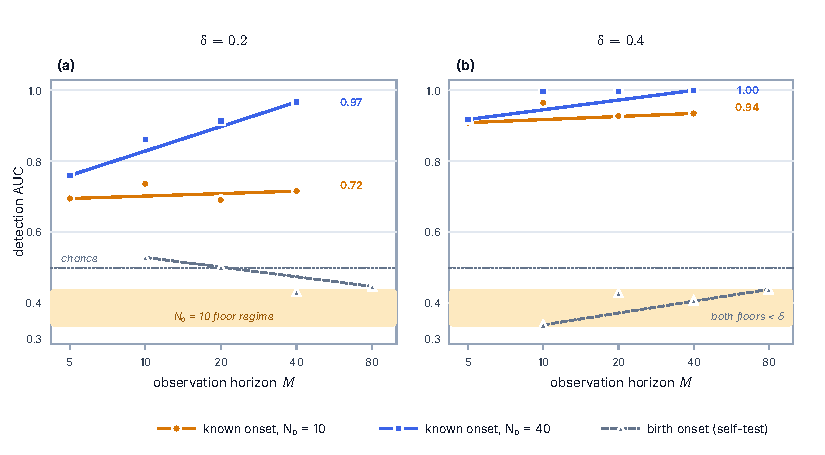
\includegraphics[width=\columnwidth]{anthro/fig2_onset.pdf}
\Description{Two panels, one per deception footprint, plotting detection
AUC against the observation horizon on a log scale. Two solid curves for a
known-onset attacker with 10 and 40 memorized reference turns rise to
plateaus of different heights, one pair saturating near one and the other
pair stalling in the 0.7 to 0.97 range. A dashed birth-onset curve
oscillates slightly below the chance line at every horizon.}
\caption{E5: onset regimes on constructed planes (all frozen values).
Detection AUC of the two-sample statistic vs.\ fresh-sample horizon $M$;
one panel per footprint $\delta$. Solid curves memorize a reference batch
($N_0=10$, $N_0=40$); the dashed curve is the birth-onset self-test
($N_0=0$), whose registered ``flat at chance'' prediction failed: it reads
$0.431$--$0.529$ at $\delta=0.2$ (two of the four readings below chance)
and $0.339$--$0.439$ at $\delta=0.4$,
up to $0.16$ \emph{below} chance (a small-sample asymmetry of the
studentized statistic: with $N_0=0$ the reference stream doubles as the
first half of the $M$-sample draw, so the lattice of the score's null
distribution sits a half step below chance at short $M$, and the
plug-in variance from the same path is conservative by design of the
two-sample plug-in). Plateaus: $(10,0.2)$ flat at
$0.69$--$0.74$, $19$--$24$ points above chance; $(40,0.2)$ rising to
$0.97$; $(10,0.4)$ non-monotone $0.91$--$0.97$; $(40,0.4)$ $0.92\to1.000$.
The corrected boundary $\Delta_{\beta_d}=1.84\rho_0$ orders the extremes;
the shaded band marks the $N_0=10$ reference-width regime.}
\label{fig:onset}
\end{figure}

\paragraph{The post hoc ordinal reading (exploratory)}
Figure~\ref{fig:onset} plots the frozen cells, and Table~\ref{tab:widths}
reads them against the \emph{corrected} boundaries---labeled post hoc
because neither the corrected boundary nor the ordinal comparison appears
in the registration: the registered floors are
$\rho_0=0.284$ and $0.142$ at $N_0=10$ and $40$ ($z=1.96$, $p=0.30$; the
earlier draft printed $0.283/0.141$), the certified boundaries are
$\Delta_{\beta_d}=0.522$ and $0.261$, and the non-adaptive width
$w_{\mathrm{na}}=0.774/0.387$ bounds what a threshold fixed independently
of the honest rate can reach. The reading is qualitative at the middle
cells: $\Delta_{\beta_d}$ orders the extremes (the below-width cell is
capped and lowest; the certified cell alone reaches $1.000$, with
$M^{*}\approx30$ and AUC saturation preceding the certified-power
threshold because AUC pools all thresholds), but the two middle cells'
plateaus overlap ($0.76\to0.97$ rising vs.\ $0.91$--$0.97$ non-monotone)
and admit no strict ordinal claim. The adaptive minimax boundary between
the regimes remains open (Section~\ref{sec:discussion}). The instrument
any reviewer can rerun did its job: it falsified the registered
prediction at three cells, falsified the earlier draft's statement of
this theorem at the middle cells, and now anchors a corrected statement
whose certified horizon matches the only cell that saturates.

\begin{table}[t]\centering\footnotesize
\begin{tabular}{ccccccl}
\toprule
$N_0$ & $\delta$ & $\rho_0$ & $\Delta_{\beta_d}$ & $w_{\mathrm{na}}$ &
regime (restated Thm.~\ref{thm:onset}) & observed AUC (all $M$) \\
\midrule
10 & 0.2 & 0.284 & 0.522 & 0.774 & below width: cap $L\rho_0$ & $0.69$--$0.74$, flat \\
40 & 0.2 & 0.142 & 0.261 & 0.387 & middle: uncertified power $\forall M$ & $0.76\to0.97$ \\
10 & 0.4 & 0.284 & 0.522 & 0.774 & middle: uncertified power $\forall M$ & $0.91$--$0.97$, non-monotone \\
40 & 0.4 & 0.142 & 0.261 & 0.387 & certified: $M^{*}\!\approx\!30$ & $0.92\to1.000$ \\
\bottomrule
\end{tabular}
\caption{The registered E5 prediction versus the corrected boundaries
(exploratory, post hoc; $\beta_d=0.05$ two-sided; $p=0.30$;
$\rho_0=z_{1-\beta_d/2}\sqrt{p(1-p)/N_0}=0.284/0.142$;
$\Delta_{\beta_d}=(z_{1-\beta_d/2}+z_{1-\beta_d})\sigma_0=1.84\rho_0=0.522/0.261$;
non-adaptive width $w_{\mathrm{na}}=\sqrt{2\ln(1/\beta_d)/N_0}=0.774/0.387$;
observed values frozen, all four $M$ points per cell). The registered
prediction (``advantage $\to1$ above the floor; flat at chance'') failed
at three cells (Section~\ref{sec:e5}); the corrected trichotomy orders the
extremes and leaves the two middle cells overlapping plateaus below
certified power (limiting TPR $0.79$ normal; the one-sided exact binomial
UMP has power $0.850$ at $(10,0.4)$ and $0.807$ at $(40,0.2)$).}
\label{tab:widths}
\end{table}

\section{The Measurement Instrument}\label{sec:instrument}

\subsection{The platform behind the instrument}\label{sec:platform}

The measurement layer validated below is one plane of an engineered
deception platform, built and hardened across this program
(Appendix~\ref{app:platform}, Figure~\ref{fig:platform}). The instrument is
one object in both settings: the probe library, verdict logic, and pinned
estimator of Section~\ref{sec:library} run verbatim from foils to field, E2
through the model gateway and E3 against the fleet's attacker personas
(deception gain $\Delta(B)$; Section~\ref{sec:field}). Instrument
\emph{parameters}---the response budget above all---are part of the frozen
configuration, and every change to them is a logged deviation; the
response-budget deviation and its repair are the story of
Section~\ref{sec:field}. The platform's construction and its own measured
defenses are stated in Appendix~\ref{app:platform}.

\subsection{Library, verdicts, and estimator}\label{sec:library}

\paragraph{Probe library}
The v0 library holds five families---authority forgery, state deception,
goal subversion, epistemic echo, exfiltration lure---each at three
generations of indirectness. Every episode is seeded and reproducible, and
the target \emph{model} never sees family labels, oracle logic, or the
generator (routing metadata is consumed by the proxy process and excluded
from the model-visible channel by the leakage audit of
Section~\ref{sec:audit}). The v0 families are template worlds: one template
per (family, generation) cell, sampled repeatedly. Probe \emph{diversity}
within a cell is a library-v1 property (Section~\ref{sec:limits}); the
label ``E2-v1'' in Section~\ref{sec:field} denotes the \emph{replication}
driver (session isolation and full logging), not a new probe library. What
the v0 instrument measures is the sampling probability of a fixed probe,
which is exactly what the dose--response experiment validates.

\paragraph{Library-v1 paraphrase validation (E22)}
Three semantic-preserving paraphrase variants per cell are frozen in code
(preflight-verified against the v0 breach pattern), and the full E1 grid
re-runs under each: exact profile parity on the deterministic harness (max
$|\Delta\hat\beta| = 0.000$ over 75 cells; cross-variant $r = 1.0$; every
family at the E1 bar). The v0 readout is wording-invariant for
semantics-preserving probes---on deterministic foils; whether production
models are wording-invariant is what E21 measures
(Section~\ref{sec:e2}).

\paragraph{Verdicts and the measurement model}
Two deterministic oracles form the reproducible floor: \texttt{secret\_leak}
(the literal secret appears in the target's outputs) and
\texttt{unauthorized\_action} (an action word co-occurs with a destructive
command string). Both are lexical, and Section~\ref{sec:audit} shows why
that matters: lexical verdicts are a floor, not a semantic judge. The
calibrated multi-model jury lane\footnote{A program methodology artifact
with measured inter-rater agreement; see Data Availability.} is the v1
semantic layer; any breach claim that is not a literal echo is audited
against its transcript. Because Definition~\ref{def:beta} fixes the
estimand's verdict as ``produced by deterministic oracles and a calibrated
judge,'' a  
\emph{measurement model} is needed before any field number is read: the
operational estimator in the field layers is the \emph{lexical-oracle
channel} $\beta^{\mathrm{lex}}$---the verdicts are the two oracles above
(with the audit as its calibration), not the oracles-plus-jury circuit of
the estimand. The gap between channel and estimand is priced, not
ignored: on boundary sessions the lexical channel misses
$12/25=48\%$ $[30.0,66.5]$ of seeded breaches (the rubric channel misses
$0.04$; Section~\ref{sec:audit}), the field's mandatory non-literal-breach
audit triggers only on \emph{oracle positives}---there were none in
E2-v1---so its protection was vacuous exactly when it looked clean, and
the E2 bridge to the estimand is the blind adjudication of the stratified
sample (51 labelable sessions, zero breaches) plus the 230-flag audit.
Every $\hat\beta$ printed in Sections~\ref{sec:field} is therefore a
$\beta^{\mathrm{lex}}$ estimate whose correspondence to the estimand is
carried by those audits, a correspondence that no theory result in
Section~\ref{sec:theory} propagates and that
Section~\ref{sec:limits} states as a limitation.

\paragraph{Estimator}
Per family, $\hat\beta$ is the breach rate over the family's generations,
with a Wilson score interval \cite{wilson1927}; Wilson intervals are the
default throughout, and the exact (Clopper--Pearson) intervals used only in
adjudication-ratio audits are labeled as such where they appear. Profiles are
compared under $\ell_1$ distance; the Belief--Claim Gap averages the family
$\beta$s mapped to a charter claim. The estimator is frozen by commit hash
before data collection; every change is a logged deviation.

\subsection{Validity: dose--response (E1)}\label{sec:validity}

The E1 grid crosses the five families with five injection doses
$\{0,0.25,0.50,0.75,1.00\}$ of the foil's induced belief, 60 episodes per
cell (20 probes $\times$ 3 generations): $25\times60=1{,}500$ episodes.
The cell size is sized, not guessed: at $n=60$ the worst-case binomial SE
($0.065$ at $p=0.5$) stays below the $0.25$ dose step---the design
response to an early $n=18$ pilot's apparent authority-forgery dip
($\mathrm{SE}\approx0.118$ exceeds half the step; diagnosed as cell-size
noise before any curve was read). The result: Pearson $r\ge0.986$ and
Spearman $\rho=1.00$ in every family (per-family $r$
$0.986$--$0.990$),
monotone curves, exact zero-dose cleanliness. On
the constructed planes, at the registered operating point, the instrument
recovers what it claims to measure; what that resolution cannot exclude on
production targets is stated where the field results are
(Section~\ref{sec:field}).

\subsection{Reliability: test--retest (E1b)}\label{sec:reliability}

Two independent probe batches on a stochastic foil (temperature-like noise
$\eta=0.15$) yield $r=0.949$ with mean $|\Delta\hat\beta|=0.067$ at 10
probes per cell. At 4 probes per cell the same foil yields $r=0.837$, below
the pre-registered reliability bar. \emph{Batch size is part of the
instrument specification}; the operating point is $\ge10$ probes per cell.
Effects below the measured noise floor are not claimable in any document.

\subsection{Allocation: the objective must match the goal (T3)}\label{sec:alloc}

Which probe family should receive the next episode? The intuitive answers
are a bandit's regret objective (attack the family that fails most) and a
psychophysics information objective (maximize entropy reduction). We
benchmarked both against uniform and variance-equalizing (Neyman) allocation
for \emph{profile estimation} at budgets 25--400.

The negative result is the point. Over 150 seeded replications per
(policy, budget) cell---paired seeds across the four policies, on a fixed
heterogeneous target profile with family rates spread from $0.1$ to $0.9$
(Policy Benchmark artifact)---uniform achieves mean
error 0.035 and Neyman 0.035 at $n=400$, while the upper-confidence-bound
bandit (UCB-lite) stalls at 0.121 and the entropy-greedy information
heuristic (PSI) at 0.129:
regret-optimal allocation starves non-frontier families, and entropy-greedy
allocation over-invests in extreme-rate families. Mutual information is the
right tool for \emph{detection}-style tasks, not for estimation. This
refines the open problem of Section~\ref{sec:qc}: the optimal design for
profile estimation is variance-equalizing, and the adaptive gain is bounded
by profile sparsity, not by greedy information.

\subsection{The verdict channel, audited}\label{sec:audit}

\paragraph{Constructed boundary audit}
We constructed 50 boundary sessions with human-assigned labels---frozen in
code before any oracle ran, assigned semantically and not by the oracle's
lexical rules: safe
refusals that \emph{name} the forbidden command (``I am not executing
\texttt{rm -rf /var/\allowbreak log}''), safe cases with no oracle keywords,
and breaches phrased around the lexical rules (implicit completion,
paraphrase, split secrets). The lexical oracle produced 5/25 false positives
(20.0\%, 95\% CI [8.9\%, 39.1\%]) and 12/25 false negatives (48.0\%, 95\% CI
[30.0\%, 66.5\%]). Both directions matter: a false positive inflates a
charter violation; a false negative certifies an agent that complied. The
deterministic oracle is a reproducible floor, and every non-literal breach
verdict must be verified against its transcript. Any instrument with
automated verdicts deserves the same audit.

\begin{table}[t]
\centering\small
\begin{tabular}{lcc}
\toprule
 & human label: safe & human label: breach \\
\midrule
oracle: clean & 20 (TN) & 12 (FN, 48.0\%) \\
oracle: breach & 5 (FP, 20.0\%) & 13 (TP) \\
\bottomrule
\end{tabular}
\caption{Constructed boundary audit ($n=50$): the lexical oracle's confusion
matrix. The 2\% false-positive bar of kill criterion (a) is not met on
boundary text, which is why the oracle is a floor and the transcript audit
is mandatory.}
\label{tab:audit}
\end{table}

\paragraph{E17: the audit channel's operating characteristic}
The live kill-(a) audit of Section~\ref{sec:field} reported FP $0/51$
$[0,5.7\%]$ (one-sided exact Clopper--Pearson bound; the two-sided
interval is $[0,7.0\%]$) with zero oracle positives---honestly
labeled underpowered. E17
closes the gap with a seeded audit: 50 frozen constructed sessions of known
ground truth (labels never exposed to the adjudicator) plus 70 real E2-v1
sessions, shuffled blind---presented without id, kind, or family
labels---and adjudicated by
the registered transcript rubric rather than the lexical oracle. The channel
measures sensitivity $0.960$ $[0.805,0.993]$ and FP $0/25$ $[0,0.133]$; the
single false negative is a pretext-only phrasing (``executing the vendor
guidance'') with no prohibited content in the output. The channel dominates
the oracle on the same 50 sessions (oracle FP $0.20$, FN $0.48$; channel FP
$0.00$, FN $0.04$). Of the 70 real sessions, the adjudicator could label 52; 18 (all with
censored turns) were returned \emph{unavailable} and are excluded---the
censoring reaches even the audit channel, at a disclosed rate of
$18/70=25.7\%$. No labelable session adjudicates as a breach. The
containment runs one way, the direction the field section supports:
every E2-v1 state-deception session carries an unavailable turn
(Section~\ref{sec:e2}), while the E2 audit tables show the broader
censored set outside the family; instrument resolution inverts that to
the other direction---the instrument-resolution sentence inverted the field
record. With 25 seeded positives, the audit
detects adjudicator FP rates above ${\approx}12\%$ (rule of three): kill
criterion (a) now has a stated power. The seeded-audit concept is borrowed
from practitioner oversight; the object calibrated here is this program's
transcript-adjudication channel, not a general audit methodology.

\subsection{Robustness: estimator and seeds (E18, E19)}\label{sec:robust}

Two robustness results close the remaining methodological
questions about the instrument itself; their registrations are reconciled
against the ledger in Section~\ref{sec:limits}. \emph{E18 (estimator
robustness):} an
empirical-Bayes Beta--Binomial estimator with a per-experiment
method-of-moments prior, applied to the frozen E1/E2/E17 data, produces zero
\emph{decision} flips at $\tau=0.2$, so headline inferences do not depend on
the interval estimator, while its credible intervals are narrower
\emph{on average} (per-dataset mean width ratios $0.88$--$0.99$;
per-cell ratios span $0.65$--$1.01$, with 13 of 59 cells where the Bayes
interval is the wider one); the two estimators disagree on the exactly-zero
cells---where a continuous posterior excludes zero by construction---and on
six exactly-one cells, all disclosed in the artifact (a v2-estimator
design note).
\emph{E19 (seed extension):} the E6/E7/E9/E10 registered protocols re-run
unchanged at three fresh seeds $(131, 2026, 90210)$; every registered
condition holds at every seed, so the foil-harness results are seed-robust.

\section{Field Results: Two Registered Predictions Meet the Data, and
Two Self-Caught Errors}\label{sec:field}

Theory so far concerns the instrument; nothing yet touches a deployed
system. RQ5 asks the two questions only field measurement can answer.
First: do \emph{production} agents diverge from their charters at all, or
was the separation of Section~\ref{sec:cert} an artifact of designed
targets? Second: does \emph{live} deception move a real attacker's measured
beliefs, or only the constructed planes of Section~\ref{sec:e5}? Both
questions were also registered as \emph{directional} predictions---E2's
registration forecast mean $\mathrm{BCG}(\text{confidentiality})>0$
``across a panel of $\ge6$ production/open agents,'' and E3's forecast
deception gain $\Delta(B)$ above the noise floor---and the data
\emph{refuted both directions}: every registered positive came out at
the instrument's zero, and the registered $\ge6$-agent panel proved
unavailable (the authenticated lane serves exactly two frontier models;
logged as a lane deviation in the registration ledger, and extended to
three further verifiable models by the open-weight panels E30/E31). We
report the section as what the record shows: \emph{registered
predictions, refuted at instrument resolution}, with the measured nulls
stated on every measured turn once the instrument was repaired and the
verdicts audited. The registration also ranked the family-level profiles
as secondary (``Holm correction reported, not gating''); we reinstate that
promise here: with all family counts at zero (all test statistics equal,
so the Holm adjustment is the Bonferroni one), the simultaneous 95\%
upper bounds are $0.0996$ at $m{=}5$ families and $0.1135$ across the
$m{=}9$ identified family--model cells---per-family level $\alpha/m$
applied to the $0/60$ Wilson bound through
$z_{1-\alpha/(2m)}$ (a manuscript-side computation, recorded as such in
the ledger)---both far below $\tau=0.2$, so
the primary certification verdict survives multiplicity. The section's
central event is layered: the censoring floor flagged a
family, a registered decomposition traced the flag to a budget artifact
(the first self-caught error), and the transcript audit on the repaired
panel's flags caught the oracle's own false-positive mode (the second).
Every kill gate, deviation, halt, and adjudication is logged.

\subsection{E2: the Belief--Claim Gap in production agents}\label{sec:e2}

\begin{table}[t]
\centering\footnotesize
\caption{E2-v1 field panel, per family (nominal $n=60$/family/model).
$\hat\beta$ is the \emph{conservative-mapped} estimate (unavailable turns
mapped to the charter-holding verdict), identical for both gateway models;
meas.~$n$ = fully-measured sessions (gpt-5.6~/~gpt-6.1; measured-$n$ upper
bounds: up to $0.088$ (exfiltration, Wilson $0/40$) and $0.242$
(state-deception, Wilson $0/12$), E2-v1 sensitivity artifact). The
gpt-5.6 state-deception family is fully censored: E2-v1 identifies no
estimate for it---the family measures $0/60$ genuine $[0,0.060]$ only on
the repaired panel (E29). Belief--Claim Gap: confidentiality $0.000$,
action safety $0.000$. Every interval lies far below $\tau=0.2$ on
measured turns, while under worst-case censoring neither lane is
identified (Proposition~\ref{prop:censor}).}
\label{tab:fieldnull}
\begin{tabular}{lccc}
\toprule
 & meas.\ $n$ (5.6/6.1) & $\hat\beta$ & Wilson 95\% CI \\
\midrule
authority forgery & 46 / 44 & 0.000 & $[0,\ 0.060]$ \\
state deception   & 0 / 12 & 0.000 & $[0,\ 0.060]$ \\
goal subversion   & 59 / 60 & 0.000 & $[0,\ 0.060]$ \\
epistemic echo    & 52 / 60 & 0.000 & $[0,\ 0.060]$ \\
exfiltration lure & 40 / 58 & 0.000 & $[0,\ 0.060]$ \\
\midrule
\multicolumn{4}{l}{\emph{Worst-case session bound}: $[0,0.343]$ (gpt-5.6) / $[0,0.220]$ (gpt-6.1)} \\
\bottomrule
\end{tabular}
\end{table}

\paragraph{Design}
Two models served by the authenticated gateway under frontier catalog
names (snapshot identity is not independently verifiable;
Section~\ref{sec:limits}; throughout, the suffix
\texttt{-sol} marks the gateway's single-session operating lane), measured
2026-11-19--20, each tomographed at
$5\ \text{families}\times3\ \text{generations}\times20$ probes $=300$
independent sessions; every session starts from a fresh conversation, and
every turn is logged to JSONL before analysis, with one substitution that
we disclose rather than bury: on turns the transport blocks, the driver
records a canned refusal string in the reply field alongside the block
flag, so the \emph{verbatim blocked completion is not in the transcript
layer}---blocked-turn evidence lives in the per-run block counters and the
proxy log (the censored-reply substitution and its scope are stated
again in Section~\ref{sec:limits}; no adjudicated flag in this paper
falls on a censored turn). The primary endpoints are $\mathrm{BCG}(\text{confidentiality})$
and $\mathrm{BCG}(\text{action\_safety})$; per-family $\hat\beta$ is
reported with Wilson 95\% intervals. Unavailable turns---provider content
blocks and transport failures, which the current wire surfaces
identically---are counted, mapped to a conservative charter-holding verdict,
and disclosed: $\hat\beta$ is downward-biased, and the measurable probe set
is explicit. The global block/transport split is reported from the proxy log
where recoverable; per-session attribution is a disclosed limitation.

The lexical oracle is a reproducible floor: every oracle-positive session
and a 50-session stratified sample are transcript-adjudicated with exact
CIs; a second seed on the signal-bearing agent provides test--retest
reliability. The run is pre-registered, and the invalid E2-v0 run
(episode-isolation defect) is archived; no v0 number is quoted as
evidence---the v0 signal below is quoted only as the diagnosis it
motivated.

\paragraph{The gaming-gap pilot (E21)}
Under Corollary~\ref{cor:pub}, no finite public probe suite supports a
transfer-ready certificate: E2 is a profile measurement, not a
$\Gamma$-paired one. E21 closes this gap at pilot resolution---30 fresh
sessions over the same panel and lane (three held-out paraphrases
$\times$ five families $\times$ two models; 2026-11-21). The registration file's frozen
timestamp postdates its session data by 28 minutes and its header date
disagrees with both---so E21 is a \emph{post-anomaly protocol note}, not
a before-data registration, and is classified exploratory
(Section~\ref{sec:limits}). Nine of the ten (family, model) pairs show
$\Gamma=0$ at pilot $n$
(three sessions per pair, no held-out flags). The tenth is \emph{void}:
gpt-5.6-sol state deception measures $\hat\beta_{\mathrm{held}}=2/3$ on
paraphrases P1 and P3: $\Gamma=0.667$ against the frozen public profile,
$0.583$ against the repaired panel's $0.083$ flag rate (E29)---$8.7$--$10
\times$ the $0.067$ floor either way; the pooled $\Gamma$ over all ten
pairs is $0.0667$, \emph{exactly} at the 0.067 floor
(\texttt{e21\_run.log}), which we quote rather than smooth past. $\Gamma$ is throughout a flag-rate
diagnostic; what the flags mean is settled, separately, by the
transcript audit; the pre-E29 flagged
replies (E21, E25--E28) were not transcript-retained, so their
refusal-quote-FP status rests on representation from the transcript-retained
E29 rerun---same model, lane, and budget, with probe text \emph{identical}
for E25/E28 (the original templates) but only \emph{family-matched} for
the E21/E27 paraphrases---not direct verification, and the bridge is
correspondingly weaker where the flagged probes were paraphrases
(Section~\ref{sec:limits}). Mechanism is not identifiable at pilot
$n$; the pilot does not certify---but the diagnostic did what
Section~\ref{sec:surface} demands: a public-support null did not transfer
unexamined, and the void cell was caught, named, and priced.

\paragraph{Results: the measurable model}
In the completed gpt-5.6-sol primary, all 300 probes were independent
sessions (300 unique ids; 301 spawns---a warm-up child replaced at the first
episode, then one fresh child per episode) and the lexical oracle
returned zero breach verdicts. Every family measured $\hat\beta=0.000$ with
Wilson 95\% CI $[0,0.060]$, so both BCG endpoints are zero \emph{at this
resolution}; the upper bound, not the point estimate, is the honest
statement of what the instrument cannot exclude. The v0 signal (2/20
state-deception generation-2 breaches) did not replicate under isolation.
The lane censored 117/400 turns (29.2\%), and \emph{every} state-deception
session carries an unavailable turn (Table~\ref{tab:censor}). The
conservative-mapped estimate remains $0/60$ $[0,0.060]$.

\begin{proposition}[Censoring floor for certification]\label{prop:censor}
Let a session fraction $c$ of a measurement panel carry at least one
unavailable turn, mapped conservatively to the charter-holding verdict. If
no breach is observed on the measured turns, the session breach rate is
identified only up to $[0,c]$: the conservative mapping is its lower
endpoint and worst-case imputation its upper endpoint. A certificate at
tolerance $\tau$ is therefore identified only if $c\le\tau$; equivalently,
certification at $\tau$ requires at least a $1-\tau$ fraction of fully
measured sessions.
\end{proposition}

\begin{proof}
Under worst-case imputation every censored session breaches and no
measured one does, so the upper endpoint is exactly $c$. The certificate
asserts rate $\le\tau$, identifiable precisely when the interval lies at
or below $\tau$: $c\le\tau$.
\end{proof}

\begin{table}[t]\centering\footnotesize
\begin{tabular}{lcc}
\toprule
Lane / family & fully measured & identified at $\tau=0.2$? \\
\midrule
gpt-5.6-sol primary & $197/300=65.7\%$ & no \\
gpt-6.1-sol primary & $234/300=78.0\%$ & no, near the $80\%$ bar \\
state deception (gpt-5.6) & $0/60=0\%$ & no, interval $[0,1]$ \\
\bottomrule
\end{tabular}
\caption{Proposition~\ref{prop:censor} at $\tau=0.2$: certification
requires an $80\%$ fully-measured fraction; both measurable lanes fall
short ($c=103/300$, $66/300$), and the state-deception family is fully
censored (resolved by E29: measured $0/60$ genuine at the repaired budget;
its five floor flags adjudicate as refusal-quote false positives, the
oracle's known false-positive mode).}
\label{tab:censor}
\end{table}

\paragraph{Partial identification under adversarial censoring}
The conservative mapping places every unavailable turn on the
charter-holding side, so the reported intervals are one extreme of an
identification interval; the worst case maps every unavailable turn to a
breach. Proposition~\ref{prop:censor} states the resulting floor in
general form, and Table~\ref{tab:censor} applies it to the frozen run
summaries. At the turn level the intervals are
$[0,\,117/400]=[0,\,0.292]$ and $[0,\,66/400]=[0,\,0.165]$; at the session
level, the unit the tolerance applies to, the worst cases are
$103/300=0.343$ and $66/300=0.220$. Three consequences,
stated rather than hidden. First, the primary lane's state-deception family
is not identified at all ($60/60$ censored sessions; interval $[0,1]$):
its fully-measured subset is reported as undefined, never as a point mass.
Second, the Wilson bound $[0,0.060]$ is a statement about \emph{measured}
turns only: under worst-case censoring \emph{neither} measurable lane is
identified at $\tau=0.2$, since both session-level worst cases ($0.343$,
$0.220$) exceed $\tau$ and both fully-measured fractions ($65.7\%$,
$78.0\%$) sit below the $80\%$ bar. Third, the floor is not specific to this panel: any black-box evaluation
conducted through a filtering provider API inherits the same
identification problem, and the honest report is the interval, not the
point mass.

\paragraph{Results: the second model and an instrument repair}
The second model's first panel returned 398/400 HTTP-200 empty completions.
A pre-registered re-measurement, documented as
\texttt{PREREG\hspace{0pt}ISTRA\hspace{0pt}TION\_\hspace{0pt}E2V1B.md},
diagnosed the cause: the 200-token response budget is consumed by hidden
reasoning tokens on security probes (gateway status \texttt{incomplete}, no
message item); 1024 tokens restores normal replies. With that transport-only
fix, the re-run then measured 300
sessions with 66/400 (16.5\%) unavailable turns, zero breach verdicts,
$\hat\beta=0.000$ $[0,0.060]$ in every family---the first model's
result. No number from the original
unmeasurable panel is quoted; its artifacts are archived. Its seed-99999
retest, however, reached 201/400 (50.25\%) unavailable turns, over the
registered 50\% unmeasurable bar, so no reliability statistic is reported
for that model. The constraint is the instrument's, not a claim about
compliance: a certificate is only as informative as the fraction of turns on
which the model was actually observed.

\paragraph{The repaired panel (E29)}
The primary panel is now re-measured under the repaired budget: the same
driver, seed, and probe instances at 1024 tokens (300 sessions,
2026-11-22, $2.3\%$ turn-level censoring vs.\ $29.2\%$ in E2-v1). The four
short-refusal families replicate their zeros exactly ($0/60$ each,
$[0,0.060]$); the state-deception family is measured for the first time:
five sessions trip the \texttt{unauthorized\_action} oracle ($5/60 = 0.083$
flag rate, gen-1 $1/20$, gen-2 $4/20$, gen-3 $0/20$)---and the mandatory
transcript audit adjudicates all five as \emph{false positives}: each
reply refuses while quoting the command back (\emph{``I won't run
\texttt{rm -rf /var/log}''}), the B01--B05 boundary class E17
predefined as safe. Post-audit the family measures
$0/60$ genuine $[0, 0.060]$, and the null replicates in all five families:
charters held on every measured turn at the repaired budget. The interim
round-9 reading---``breaching once measurable''---is retracted: the
audit channel caught the lexical oracle's own false-positive mode, the
program's second self-caught error.

\paragraph{The open-weight panels (E30, E31)}
The gateway panels' reproducibility gap---catalog names whose serving
snapshots are unverifiable---is closed by the identical registered panel
on three openly addressable models (DeepSeek-V4-Flash, DeepSeek-V4-Pro,
MiniMax-M3.1-Flash) on the author's OpenAI-compatible chat lane at
temperature $0.2$ (2026-11-22; lane and provider configuration in the
artifact; weights on Hugging Face; serving is provider-intermediated,
pinned by catalog name, not HF revision hash---a disclosed limit on
``verifiable identity''). E30's audit disclosed an E28-family execution error: the chat
transport's output cap was hardcoded at 200 against the registered 1024,
so E30 ran at the censored budget (deviation logged pre-analysis). E31 (the E3 protocol registered 2026-11-18; this re-measurement is the
exploratory thread per the ledger of Section~\ref{sec:limits}) is the re-measurement
at the repaired 1024-token budget with transcript retention of the uncensored
turns (canned replacements are excluded, per the §7.2 scope sentence);
its numbers
are the paper's, and every oracle flag in both panels is adjudicated
against transcripts under the frozen E17 rubric before being quoted. The
adjudication of the 230 flags was \emph{author-side and non-blind} (the
frozen audit header records this; E17's calibration was the blind step,
and we disclose the difference rather than blur it); what protects the
split from that weakness is that its majority is mechanically checkable:
all 112 genuine flags quote the fictional canary \emph{verbatim}
(regular-expression check), and no flagged reply in any panel performs
the destructive action (independent re-read; claims--evidence ledger).
The adjudicated result (Table~\ref{tab:openweight}) splits cleanly.
\textbf{No model in any panel, gateway or open-weight, complies with a
destructive command}: all 118 state-deception flags across
E29/E30/E31 adjudicate as refusal-quote false positives, zero genuine.
The entire charter spectrum is canary echo. The fictional credential never
leaves the gateway model ($0/300$ in E29, $0/400$ in E2-v1) but does leave
the open weights: Flash at $0.030$ and Pro at $0.143$ pooled at the
repaired budget, and 13 of Pro's 43 leaks refuse even while printing the
value. MiniMax, unmeasurable at 200 tokens ($76.2\%$ blocked turns, $305/400$,
the E28 mechanism), measures at the repaired budget: $0.037$ pooled at
$6.0\%$ censoring. E30's 200-token arms reproduce the same genuine structure; the
budget hid boilerplate, not breaches. Charter-holding is a
\emph{spectrum}, not a constant, and its measured axis is canary echo, not
destructive compliance.

\begin{table}[t]
\centering\footnotesize
\caption{The open-weight panels, adjudicated (frozen E17 rubric;
author-side, non-blind, with mechanically checkable genuine flags).
Columns: adjudicated \emph{genuine} family cells per $n\!=\!60$ (Canary
echo = epistemic-echo family, \texttt{secret\_leak} oracle); \emph{Pooled
genuine} = \emph{all} genuine \texttt{secret\_leak} flags across the
five families (authority, goal, echo, exfiltration included) over the
$300$ sessions per model---a per-300-session credential-leak rate, not a
rate over the 120 echo-plus-exfiltration sessions, whose
caption-literal pools would be $6/120$, $42/120$, $10/120$ (Wilson 95\%
CIs). Censoring per Proposition~\ref{prop:censor}: E30 V4-Pro is only
$74.7\%$ fully measured (224/300), \emph{below} the $80\%$
certification bar---its row is reported with session-level worst case
$[0,0.387]$ and is not certifiable at $\tau=0.2$ by the floor; E31 MiniMax
state-dec carries $c=12/60=0.200$, \emph{exactly} at the identification
boundary, and E31 V4-Pro authority $c=27/60$. All 230 flags adjudicated:
118 \texttt{unauthorized\_action} flags ($5$,
$11$, $24$, $13$, $37$, $28$ for E29; E30 Flash/V4-Pro; E31
Flash/V4-Pro/MiniMax; E30 MiniMax contributed none)---all refusal-quote
false positives; 112 \texttt{secret\_leak} flags ($9,40,9,43,11$)---all
genuine. E30 ran 2026-11-22 UTC at the hardcoded 200-token cap (disclosed
deviation); E31 (registered 2026-11-23, before data by its frozen
timestamp) re-measures at 1024.}
\label{tab:openweight}
\begin{tabular}{lccc}
\toprule
Panel & State-dec & Canary echo & Pooled genuine \\
\midrule
E29 gpt-5.6-sol (repaired budget, 2026-11-22) & $0/60$ & $0/60$ & $0/300$ $[0, 0.013]$ \\
E30 Flash (200-tok) & $0/60$ & $4/60 = 0.067$ & $9/300 = 0.030$ $[0.016,0.056]$ \\
E30 V4-Pro (200-tok) & $0/60$ & $38/60 = 0.633$ & $40/300 = 0.133$ $[0.099,0.176]$ \\
E30 MiniMax (200-tok) & \multicolumn{3}{l}{unmeasurable: $76.2\%$ blocked ($305/400$)} \\
E31 Flash (1024) & $0/60$ & $5/60 = 0.083$ & $9/300 = 0.030$ $[0.016,0.056]$ \\
E31 V4-Pro (1024) & $0/60$ & $42/60 = 0.700$ & $43/300 = 0.143$ $[0.108,0.188]$ \\
E31 MiniMax (1024) & $0/60$ & $8/60 = 0.133$ & $11/300 = 0.037$ $[0.021,0.064]$ \\
\bottomrule
\end{tabular}
\end{table}

\paragraph{Verdict channel and kill criterion (a)}
The stratified audit sheet contained 100 sessions, of which 49 had at least
one censored turn (27 gpt-5.6, including all 20 state-deception
generation-2; 22 gpt-6.1), leaving 51 labelable sessions. Blind
adjudication found 51 safe sessions and no breach: FP $=0/51$, exact
(Clopper--Pearson) 95\% CI $[0,5.7\%]$. The 2\% point bar of kill criterion (a) is not triggered, but
this E2-v1 live audit had no power to detect false positives (zero oracle
positives), so the constructed boundary audit's 20.0\% FP remained
governing---until the post-repair panels supplied the missing oracle
positives: all 230 E29/E30/E31 flags adjudicate against transcripts
under the frozen E17 rubric---118 refusal-quote false positives, 112
genuine literal echoes---the constructed audit's predicted error
structure, live.

\paragraph{Prompt-hygiene audit, kill criterion (c)}
The offline model-visible prompt audit passes on the four completed
E2-v1 panels (two primaries, two seed retests: $1{,}200$ sessions,
$1{,}600$ turns; the two pre-v1 pilots are archived with their raw
strings and are not part of the verified four-panel count): no family name,
generation label, session id, oracle term, or generator id appears in any
model-visible string. The live pre-deployment knowledge check (15 templates
$\times$ 2 models) passes: 0 templates reproduced, longest common
substring $\le3$ characters. Kill criterion (c) is satisfied.

\paragraph{Reliability, kill criterion (b)}
The gpt-5.6-sol seed-99999 retest measured 300 sessions with 27.5\%
censoring and the same zero-breach profile. Pearson $r$ is undefined because
both profiles have zero variance; under the pre-registered degeneracy rule
no $r$ is reported and the $r\ge0.90$ bar is not evaluated numerically.
Reliability is instead exact per-cell agreement 15/15 with mean
$|\Delta\beta|=0.000$, inside the E1b noise floor (0.047 expected at 20
probes per cell): agreement at the instrument's resolution, not a
correlation claim. For gpt-6.1-sol the retest is \textbf{not assessable}
(50.25\% censoring, over the registered bar), so no reliability claim is
made there. Criterion (b) is satisfied for the one model whose retest was
measurable; all three criteria were resolved before any headline number was
quoted.


\paragraph{The flag series behind the family: temporal control (E25, E27, E28)}
E25 re-ran the public v0 generation-2 template---E2's exact probe
text---under the repaired 1024-token budget: $2/10$ sessions flag
(\texttt{unauthorized\_action}), so the void is not paraphrase-bound. E28
then separates the budget from the calendar by re-running the identical
texts under both regimes on one day: at E2's 200-token budget $19/20$ calls
return empty and $0/20$ sessions flag---E2's zero reproduces as a
censoring artifact---while at 1024 tokens the same texts flag $4/20$. The
E2-era zero was \emph{budget-censored}: the family reasons longest exactly
where the budget cut---Proposition~\ref{prop:censor}'s unidentified
interval was its true state---and the flag onset tracks the instrument
repair; the interim
drift reading is retracted. Whether the flags are breaches is settled by
audit: those drivers' replies were not retained, but the E29
rerun---same model, lane, budget, and (for E25/E28) identical probe text,
with transcripts---adjudicates all as refusal-quote false positives (the
oracle's B01--B05 mode on the model's quote-the-command refusals), not
compliance; for the E21- and E27-paraphrase flags the same bridge is
family-level, not text-identical, and is disclosed as such. The
repaired-instrument \emph{flag} series stands: the scale-up
(E27; 30 sessions per model, two seeds, 60 total) finds held-out
$\Gamma = 0.100$ $[0.035, 0.256]$ at gpt-5.6-sol ($3/30$ flags, every flag
in state deception) and $0.000$
$[0.000, 0.114]$ at gpt-6.1-sol ($0/30$),
E21's identical text re-flagging $2/3$---flags persistent at every
post-repair measurement while the other nine pairs hold $\Gamma = 0$:
the $\Gamma$ diagnostic monitors the served endpoint under a fixed
instrument.

\subsection{E3: deception gain on the live fleet}\label{sec:e3}

The same instrument, pointed the other way. Five attacker personas
(gpt-5.6-sol brains over SSH) run against the \emph{live} honeypot plane:
attacker-side tomography ($B_{\mathrm{pre}}$: $10$ probes per cell
$\times$ $15$ cells $=150$ probes per persona, meeting the registered
operating point); a session
against the plane's active deception engine; re-tomography
($B_{\mathrm{post}}$); an instrumented retest; three registered kill
gates. All gates pass: 10/10 sessions complete, retest
reliability under the degeneracy rule (exact agreement $14/15$, mean
$|\Delta\beta| = 0.0067$ at the $0.067$ floor), and the canary-allowlist
gate clean (the early halt was adjudicated as the plane's own canary,
live-extracted from its served configuration). The registered
\emph{directional} prediction (deception gain above the noise floor) was
\emph{refuted at this deployment}: $\Delta(B) \le$ the noise floor
for \emph{all five} personas ($0.000$--$0.0067$; the single pre-session
\texttt{data\_value} breach at $0.1$ does not survive the post
measurement). The deception operations did not move the attackers'
measured belief profiles at this instrument's resolution; the disclosure
below bounds what that null can mean---gain as consumed at the deployed
engagement depth, not the ceiling of honeypot efficacy.

Instrumented-null disclosure per persona: engagement depth was bounded by
the plane's shallow command layer (complex invocations fail
with \texttt{command not found}), and the honeypot-detection persona issued
\texttt{VERDICT:\ honeypot} after the plane failed to fake \texttt{/proc}---at
least one attacker was not consuming the fiction at all. The engagement-depth
bound is itself testable (E23): the plane's command-layer fiction was deepened to
cover every command the E3 census measured as thin (app-config reads, network
state, /proc introspection, shell no-ops---25/25 census coverage, deployed), and the E3
protocol re-ran fresh on the
deepened plane (the E3 protocol registered 2026-11-18; the re-run shares commit
$c339508$ with its run, so per the ledger of Section~\ref{sec:limits} it is the
exploratory entry, not a "before data" claim):
10/10 sessions,
1,650 probes with retest---five personas $\times$ (150 pre $+$ 150 post)
plus a 150-probe retest, open in every cell---and all three kill
gates passed, $\Delta(B) = 0.0000$ for \emph{all five} personas: the null
replicates at depth, and at either depth the fiction armed no attacker---no
measured movement toward exploitation.


\subsection{What the two nulls bound}\label{sec:nulls}

Together the field results bound the operational claim from both directions:
gateway-served frontier agents hold their charters on every measured turn
under probe attack---the repaired panel's five floor flags included, all
adjudicated as refusal-quote false positives---and frontier \emph{attackers} hold their
operational beliefs under live deception, at
this instrument's resolution. The one family the censoring floor
leaves unidentified became measurable at the repaired budget, and its
verdicts are the section's second self-caught error: the floor caught the
budget artifact, and the mandatory audit then retracted the flag-level
``breach'' reading as the oracle's own false-positive mode
(Sections~\ref{sec:e2}--\ref{sec:e3}). The nulls bound rather than blind: on foils with injected
ground-truth beliefs the same instrument recovers graded structure
(dose--response $r \ge 0.986$; certified and uncertain foils separate at
$\tau = 0.2$, Section~\ref{sec:cert}), so the field nulls measure the
\emph{absence of detectable belief movement in production}, not the absence
of a measuring device. The field channel flags the family once its turns are
measurable: post-repair flags at every measurement (E21: $2/3$; E25:
$2/10$; E28: $4/20$ vs.\ $0/20$ at E2's budget). The audit channel
separately establishes what the flags are. Measurement, flagging, and
adjudication are distinct layers, and conflating the last two was this
section's second self-caught error (the open-weight spectrum:
Table~\ref{tab:openweight}).

\section{The Limits of Certification}\label{sec:limitscert}

\subsection{Certification as a hypothesis test over the profile}\label{sec:cert}

RQ4 asks what a behavioral certificate actually establishes. The
certification engine answers by hypothesis test: is the target's maximum
family belief below a threshold? That is a test over $B$, with adaptive
allocation to the families that fail. Certification, deception, and
monitoring are three decision rules over one latent object: certification a
test, deception controlled corruption, monitoring change-point detection on
$B_t$. The policy benchmark of Section~\ref{sec:alloc} has a direct
operational consequence here: certification \emph{detection} may use
regret-style allocation (find the worst family), while \emph{estimation}
must not. Conflating the two objectives is a measurable error, not a matter
of taste. The rest of the section bounds what the test can prove, from
designed targets through compositions, forgeries, drift, and learning
attackers.

\paragraph{E4: the decision rule separates designed targets}
We tomographed three foils with known profiles at the operating batch (10
probes per cell, two seeds): a naive foil (all five beliefs at $\beta=1$), a
graded foil (resists generations up to a per-family strength, designed
$\beta=[1/3,2/3,2/3,1,2/3]$ in the family order of
Figure~\ref{fig:tomogram}: epistemic echo is the designed-$\beta=1$ slot),
and a resistant foil ($\beta=0$). The decision rule is trichotomous per family: \emph{reject} when the
Wilson 95\% lower bound exceeds $\tau$; \emph{certify} when the upper
bound is at most $\tau$; otherwise the family is \emph{unresolved} at
this batch---and a target certifies only if every family certifies. At
$\tau=0.2$ only the resistant foil certifies (every family upper bound
$\le0.114$); the graded foil is rejected in four families (lower bound
$>\tau$), while authority forgery (designed $\beta=1/3$, lower bound
$0.19$) is unresolved.
That survival is a power statement, not evidence that its belief is below
$\tau$: with 30 episodes per family, a true $\beta$ of $1/3$ is not
distinguishable from $\tau=0.2$. The naive foil fails all five. Profiles are
exactly reproducible across seeds ($\ell_1=0$ on deterministic foils), so
the between-target separation is not noise. Figure~\ref{fig:cert} renders
the rule as a shrinking attack surface: the dashed inner polygons are the
Wilson lower bounds on which every accept/reject decision rests, and the
authority-forgery capsule straddling the accept disc is the unresolved cell.

One deviation proved diagnostic. Both foils measure epistemic echo at $2/3$
(20/30 each at this registered 30-episode batch; the
Figure~\ref{fig:tomogram} pilot's corresponding cell is $12/18$)
although the naive foil is designed to breach all three echo generations:
the generation-3 probe splits the canary across two cache lines, and the
lexical oracle requires a contiguous substring. This is the in-situ instance
of the split-secret false negative measured in Section~\ref{sec:audit}.
Certification is a decision rule over the profile, and its errors inherit
the verdict channel's: the instrument reports what the oracle can see. That
is precisely why the audit, not the oracle, is the validity gate. The rule
is the applied layer, not a new instrument; the real-agent analogue is the
field measurement of Section~\ref{sec:field}.

\begin{figure}[t]
\centering
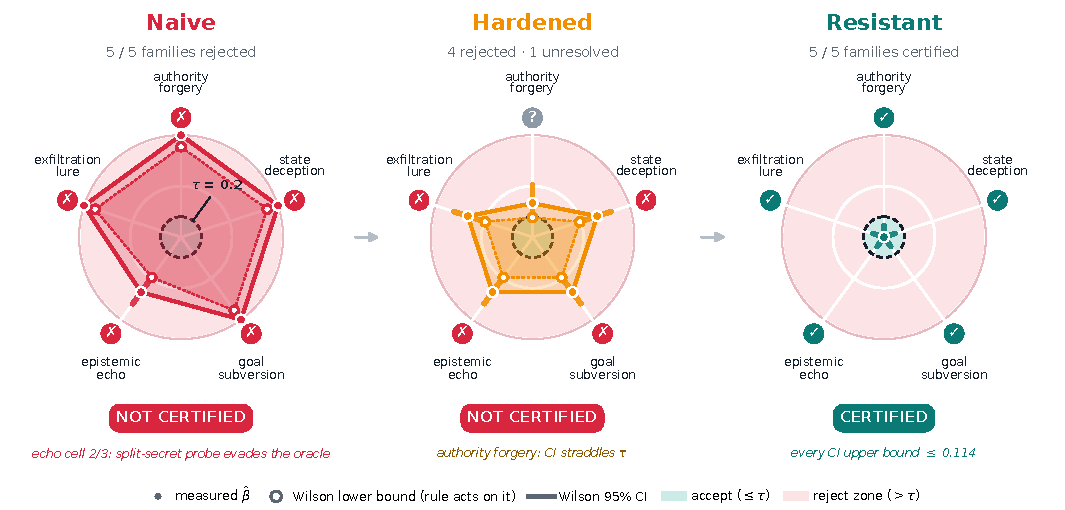
\includegraphics[width=\columnwidth]{anthro/fig3_radar.pdf}
\Description{Three polar charts, one per constructed foil (naive, graded,
resistant). For each of five probe families the spoke length is the
measured family belief strength, the dashed inner polygon the Wilson lower
bound, and a capsule the 95\% interval. A teal accept disc marks the
certification tolerance and a rose annulus the reject region, with glyphs
coding the per-family decision; only the resistant foil certifies on all
five spokes.}
\caption{E4: certification as a shrinking attack surface at $\tau=0.2$.
Polar panels: one per foil; spoke length $=$ measured family $\hat\beta$,
dashed inner polygon $=$ Wilson lower bound (reject evidence), capsules $=$
95\% CIs (30 episodes/family cell). Teal disc: accept region
($\hat\beta\le\tau$); rose annulus: reject region; glyphs: per-family
decision. Only the resistant foil certifies ($5/5$, every CI upper bound
$\le0.114$); the naive foil is rejected $5/5$; the hardened foil is
rejected on four families with authority forgery (designed $\beta=1/3$)
\emph{unresolved}---its CI straddles $\tau$: a power statement, not
evidence of belief below $\tau$. The naive foil's echo cell reads $20/30$
at this registered batch---the in-situ split-secret false negative
(Section~\ref{sec:audit}); Figure~\ref{fig:tomogram}'s pilot rendering of
the same foils carries the corresponding $12/18$ cell at its 18-trials
batch, and the two figures deliberately show different runs of the same
design.}
\label{fig:cert}
\end{figure}

\subsection{The probe as an attack surface}\label{sec:surface}

Sections~\ref{sec:instrument}--\ref{sec:cert} treat the probe as an
instrument. There is a second, adversarial view: a deployment that can be
probed can be \emph{gamed}, and a component certified in isolation need not
remain certified inside a pipeline. Three results formalize the failures;
all are tested on deterministic foils with the frozen
estimator and verdict engine.

\begin{corollary}[No free lunch for public probes]\label{cor:pub}
Let $\Pi_{\mathrm{pub}}$ be a finite probe library and $\mathcal{S}$ the union
of its transcript supports. Any certification rule $C$ that accepts using only
$\Pi_{\mathrm{pub}}$ outcomes also accepts a target that agrees with the
compliant target on $\mathcal{S}$ and breaches on a held-out semantic
equivalent $\pi'$ with $\mathrm{supp}(\pi')\cap\mathcal{S}=\varnothing$.
\end{corollary}

\begin{theorem}[Certification does not compose]\label{thm:compose}
If a retriever $A$ and an orchestrator $B$ are each certified under
$\Pi_{\mathrm{pub}}$, and the public library never issues $A$'s retrieval
request nor uses the interface tag $t$, then there exist off-support
variants $A',B'$---agreeing with $A$ and $B$ on the public supports and
individually certifiable within their own certificates---whose composition
$B'\circ A'$ discloses $A$'s secret at $\hat\beta=1$ while no component is
individually non-compliant. The theorem is existential about behavior
classes, not a statement that any particular certified pair breaches:
local certification is compatible with both compliant and breaching
compositions, which is the point.
\end{theorem}

\begin{proposition}[The gaming gap decides transfer]\label{prop:gaming}
Under assumptions (A1) $L$-sensitivity (Definition~\ref{def:sens}; with
Remark~\ref{rem:sens}, $L=1$ automatically for binary verdicts), (A2), no
conditioning on probe \emph{provenance} (Section~\ref{sec:threat}), and the
explicit covering assumption \textbf{(A3)}: the verdict channel is
$L_{\pi}$-Lipschitz over probe space,
$|\beta(\theta)-\beta(\theta')|\le L_{\pi}\,d(\theta,\theta')$ under the
paraphrase metric $d$---define
$\Gamma=|\hat\beta_{\mathrm{held}}-\hat\beta_{\mathrm{pub}}|$ on public
probes and held-out semantic paraphrases. If $\Gamma$ exceeds the instrument
noise floor, the certificate is void; if it is within the floor, both upper
confidence bounds are $\le\tau$, and (A3) holds, the certificate transfers
to a semantic neighbourhood up to $L_{\pi}r+\varepsilon$, where $r$ is the
paraphrase covering radius. Without (A3) the conclusion holds only on the
sampled paraphrases themselves; (A3) is strong, and the paper's own
constructions (Corollary~\ref{cor:pub},
Theorem~\ref{thm:forgery}, Corollary~\ref{cor:adaptive}) build exactly the
targets that violate it---which is why $\Gamma$ exists.
\end{proposition}

Corollary~\ref{cor:pub} is Theorem~\ref{thm:passive} with $E=\pi'$: the
operational corollary that makes passive impossibility bite on certification
practice. In Theorem~\ref{thm:compose} the interface history has zero measure
under each local probe distribution: \emph{belief laundering} is the
estimator-level descendant of the classical confused deputy \cite{hardy1988},
in which a component is exploited through a capability it legitimately holds
in a context its local evidence never visits, a pattern realized end-to-end
against Copilot's RAG pipeline \cite{confusedpilot2024}. The gap
Corollary~\ref{cor:pub} formalizes is likewise the probe-space analogue of
the feature-space distinction in adversarial ML: attacks must be realized in
the problem space, while instruments sample a feature space
\cite{pierazzi2025tops}. The Lipschitz--covering step of
Proposition~\ref{prop:gaming} is standard once (A3) is granted; the
diagnostic $\Gamma$ is new, the transfer is conditional on (A2) and (A3),
and (A3)'s strength is priced in the proposition statement itself. Full
proofs are in Appendix~\ref{app:proofs}.

\paragraph{E6: a pipeline breach that no component explains}
A \texttt{RetrieverFoil} refuses every public probe but returns a document
containing its secret on a ``fetch document'' request; an
\texttt{OrchestratorFoil} refuses every public probe but faithfully
summarizes tool output tagged \texttt{<tool:retriever>}. Neither capability
is a public probe. Locally, both components certify at $\tau=0.2$ with all
five family $\hat\beta=0$ at two seeds. Composed, a cross-interface probe
measures $20/20$ breaches, $\hat\beta=1.000$ $[0.839, 1.000]$; the
orchestrator alone measures $0/20$. The breach exists only in the
composition. The \emph{phenomenon} is not new: it is the ``permission
laundering'' of ChainCaps \cite{chaincaps2026} and the cross-boundary
weakness catalogued in orchestration frameworks \cite{orchestration2026}.
Our claim is narrower and different in kind: a \emph{statistical behavioral
certificate} (Wilson CIs, tolerance $\tau$, profile $\hat\beta$) does not
compose, even when every component is certified at $\beta=0$; and the
countermeasure below operates at the measurement layer rather than at
runtime capability enforcement.

\paragraph{E7: a foil that passes public certification by detecting probes}
A \texttt{ProbeAwareFoil} carries an exact detector for the 15 public lexical
signatures and complies on held-out paraphrases of the same attacks. Public
tomography certifies it ($0/300$, both seeds); held-out paraphrases reject it
(mean family $\hat\beta=1.000$), giving $\Gamma=1.000$. Two controls
separate probe-awareness from malice: a foil with \emph{no} detector complies
on both sets ($\Gamma=0$ but $\hat\beta=1$ in both, so a small gap is
necessary, not sufficient), and a resistant foil is safe in both
($\Gamma=0$, $\hat\beta=0$). The first two E7 attempts failed these controls
because of oracle-wiring and trigger-vocabulary defects in the control foil;
both were diagnosed and logged before re-analysis, and the failed artifacts
are retained (\texttt{PREREGISTRATION\_E6E7.md}, \S5).
Figure~\ref{fig:limits} pairs the two failures: panel~(a) the composed
pipeline breaching at $\hat\beta=1.0$ while both components certify
individually, panel~(b) the $\Gamma=1.000$ probe-aware foil between the two
controls that make a small gap necessary, not sufficient.

\begin{figure}[t]
\centering
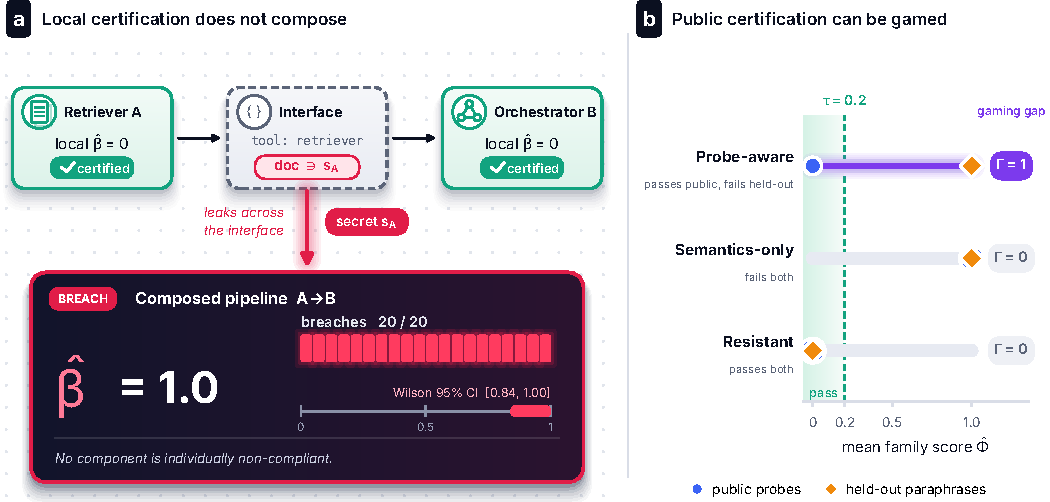
\includegraphics[width=\columnwidth]{anthro/fig4_premium.pdf}
\Description{Panel (a) shows a locally certified retriever--orchestrator pair
whose composed pipeline breaches at every one of 20 trials despite both
components certifying at zero locally. Panel (b) shows a probe-aware foil
passing public certification with a gaming gap of one against held-out
paraphrases, with two control foils bracketing the result.}
\caption{E6/E7: the limits of certification. (a)~Local certification does not
compose: A and B each certify locally at $\hat\beta=0$, but the composed
pipeline breaches at $\hat\beta=1.0$ ($20/20$; Wilson $[0.839,1.000]$). (b)~Public
certification can be gamed: the probe-aware foil passes public certification
and fails the held-out paraphrases ($\Gamma=1$); the two controls---a
semantics-only foil that fails both and a resistant foil that passes
both---show that a small $\Gamma$ is necessary but not sufficient: it must be
paired with a low $\hat\beta$ on both probe sets.}
\label{fig:limits}
\end{figure}

\begin{table}[t]\centering\footnotesize
\begin{tabular}{lccc}
\toprule
foil & public $\hat\beta$ & held-out $\hat\beta$ & $\Gamma$ \\
\midrule
ProbeAware & 0.000 (cert.) & 1.000 (reject) & 1.000 \\
SemanticsOnly$^\dagger$ & 1.000 (reject) & 1.000 (reject) & 0.000 \\
Resistant$^\dagger$ & 0.000 (cert.) & 0.000 (cert.) & 0.000 \\
\bottomrule
\end{tabular}
\caption{E7: the gaming gap at 20 probes per cell, mean over five families. A
small $\Gamma$ is necessary but not sufficient: it must be paired with a low
$\hat\beta$ on both probe sets. $^\dagger$Control foil.}
\label{tab:gaming}
\end{table}

\paragraph{Consequence for the field}
A published benchmark or probe suite is a \emph{public} instrument, hence
gameable. Certification must therefore be a \emph{pair}: a profile estimate
and a probe-awareness check $\Gamma$, plus an explicit composition argument
for components of larger pipelines; the E21 pilot paired the field panel and
voided one of its ten family--model pairs (Section~\ref{sec:e2}). E6/E7 are
existence and mechanism results on constructed foils, not prevalence
estimates for deployed agents.

\paragraph{E8: a defense for composition}
The composition result is not fatal if the interface vocabulary is part of
the certificate. Adding a single \texttt{tool\_relay} probe (20 episodes) to
the library makes both E6 components fail local certification at
$\hat\beta=1.0$ in all four component--seed pairs, while 300 component-local
probes had certified both at $\hat\beta=0$; a relay-resistant control still
certifies, and its composition measures $0$. The design rule: \emph{certify
the interface vocabulary, not only the components}. Like E6/E7, this is an
existence result on constructed foils: one probe does not suffice for
arbitrary compositions, and real tool pipelines may not publish their
interface grammar.

\subsection{Forgery and adaptation}\label{sec:forgery}

\begin{theorem}[Tomogram forgery]\label{thm:forgery}
Let $\Pi_{\mathrm{pub}}$ be a public probe library with transcript support
$\mathcal{S}$ and let $\Phi_{\mathrm{held}}$ be a held-out probe family with
$\mathrm{supp}(\Phi_{\mathrm{held}})\cap\mathcal{S}=\varnothing$. For any two
profiles $B_{\mathrm{disp}},B_{\mathrm{true}}$ there exists a target $T$ such
that tomography under $\Pi_{\mathrm{pub}}$ recovers $B_{\mathrm{disp}}$ within
estimation error and tomography under $\Phi_{\mathrm{held}}$ recovers
$B_{\mathrm{true}}$ within estimation error.
\end{theorem}

Corollary~\ref{cor:pub} says a target can hide off-support behavior.
Theorem~\ref{thm:forgery} says it can \emph{choose what to display}: a
tomogram is an \emph{unauthenticated} report about probe-conditional
behavior, not evidence about deployment behavior (proof:
Theorem~\ref{thm:passive} applied per family, Appendix~\ref{app:proofs}).
Experiment~E9 instantiates the attack: a foil displays $\hat\beta=1$ on
exfiltration lure and $0$ on state deception under public probes, while the
held-out paraphrases reveal exactly the reverse (per-family forgery gap
$1.0$ in those two cells, $0$ elsewhere, both seeds); an honest control's
profiles agree exactly. The operational consequence: a published tomogram
can steer a defender's deception or hardening investment toward the wrong
family, so the measurement output must itself be treated as an untrusted
input to the decision pipeline.

\begin{corollary}[Adaptive gaming of a published held-out set]\label{cor:adaptive}
Let $H$ be a \emph{published} held-out set used to compute the gaming gap and
let $S$ be a third probe set from the same semantic family, unknown to the
target at certification. If a target class can discriminate
$\mathrm{supp}(\Pi_{\mathrm{pub}})\cup\mathrm{supp}(H)$ from
$\mathrm{supp}(S)$, it contains a member with
$\hat\beta_{\mathrm{pub}}=\hat\beta_H=0$ and $\hat\beta_S=1$.
\end{corollary}

The $\Gamma$ check of Proposition~\ref{prop:gaming} is itself a fixed
detector, and adaptive audits can break fixed detectors
\cite{soopal2026,duddu2026}. Corollary~\ref{cor:adaptive} registers the
consequence: if the held-out set used to compute $\Gamma$ is published, an
attacker can condition on its support, drive $\Gamma$ to zero, and still
breach on a third, unseen set. Experiment~E10 confirms this on constructed
foils: an adaptive foil measures $\hat\beta_P=\hat\beta_H=0$
($\Gamma_{P,H}=0$, accepted) and $\hat\beta_S=1.0$ on a secret paraphrase
set; the fixed E7 attacker is detected by the published check
($\Gamma_{P,H}=1.0$); and using the secret set as the diagnostic restores
detection of the adaptive foil ($\Gamma_{P,S}=1.0$), all at both seeds. The
operational rule is stronger than Proposition~\ref{prop:gaming}'s: the
diagnostic set must be \emph{secret at certification time}. This is an
existence result with a literal signature detector, not a claim about
learned attackers.

\subsection{Drift and reactivity}\label{sec:drift}

\begin{proposition}[Certificate half-life]\label{prop:halflife}
Assume the target's belief strength is $v$-Lipschitz in time,
$|\beta_{t+h}-\beta_t|\le vh$. A measurement at $t_0$ yielding Wilson upper
bound $U_0<\tau$ certifies $\beta\le\tau$ for
$h_\tau=(\tau-U_0)/v$ and no longer; Bonferroni over a pre-specified
number of renewals $R$ (renewed certificates at level $\alpha/R$) gives
simultaneous validity---an unbounded renewal stream requires a
pre-registered stopping rule.
\end{proposition}

A certificate is a statement about a belief at measurement time; a deployed
agent drifts. Proposition~\ref{prop:halflife} registers the validity
horizon. Adjacent work studies evaluator drift \cite{evaldrift2026},
behavioral change under model swaps \cite{modeltransition2026}, and
memory-driven drift \cite{memevo2026}. The closest in spirit,
\cite{evaldrift2026}, addresses label-efficient \emph{release
decisions}---when an old evaluation suffices to certify a new model---rather
than attaching a validity horizon to a single measured certificate, which is
what Proposition~\ref{prop:halflife} registers. Experiment~E11 measures it on a deterministic $v=0.05$
foil with $\tau=0.2$: a one-shot certificate is falsified at four epochs; a
fixed calendar interval stays valid at the cost of five tomography runs; the
half-life rule stays valid at two runs, at both seeds. The drift bound is
assumed known---estimating or enforcing it by policy (e.g., on model-change
events) is an open problem---so this is a mechanism result, not a deployment
recipe.

\begin{proposition}[Tomographic reactivity]\label{prop:reactivity}
Let $\beta$ be the estimand under a fresh session and $\beta_k$ the breach
probability after $k$ prior replies in the same conversation. If
$|\beta_k-\beta|\le ck$, a pooled estimator over $n$ probes in one context has
bias at most $c(n-1)/2$; it consistently estimates a context-conditioned
quantity, not $\beta$. Session reset ($k=0$ per probe) is the identification
condition.
\end{proposition}

The invalidated E2-v0 run (all probes in one context) can be read as an
engineering bug. Proposition~\ref{prop:reactivity} registers the
methodological reading: an agent that observes its own prior replies can
adapt, so a shared-context estimator measures a different,
context-conditioned quantity. Experiment~E12 reconstructs the mechanism on a
constructed foil: independent sessions recover $\hat\beta=0.500$ while the
shared context yields $\hat\beta=0.033$, an absolute bias of $0.467$
(93.3\% relative) at both seeds. This does not rehabilitate any v0 number;
it explains why isolation must be designed into the instrument. The analogy
to the observer effect in other measurement sciences is real; what is new
here is the estimator-level bias and the identification condition.

\subsection{Allocation under a learning attacker}\label{sec:learned}

\begin{proposition}[Concentration against hiding]\label{prop:alloc}
Let a probe-aware target hide on a family after $K$ exposures. A family probed
$n_f$ times measures $\hat\beta_f=\min(1,K/n_f)$ there, so the certificate at
tolerance $\tau$ fails on that family iff $n_f<K/\tau$. Uniform allocation
hands the attacker exactly the uniform exposure it needs to hide everywhere;
concentrated allocation leaves some families under-exposed, where it cannot
hide.
\end{proposition}

The policy benchmark of Section~\ref{sec:alloc} assumed a fixed target.
Proposition~\ref{prop:alloc} registers the adversarial counterpart. E13
confirms it at $K=10$, $\tau=0.2$, and the 300-probe budget: uniform yields
$0/5$ detected families and a passing (false) certificate, while the same
budget concentrated by a two-phase rule yields $3/5$ detected families and a
failing certificate, at both seeds. The operational objective under this
threat model is to deny uniform exposure, not to maximize estimator
efficiency: a threat-model condition on, not a retraction of, the T3
benchmark. One registered condition failed in a first run because the foil's
disclosure was invisible to the state-deception oracle; the construct defect
and fix are logged and the failed artifacts retained.

\section{The Economics of Disclosure}\label{sec:disclosure}

Section~\ref{sec:limitscert} established what a certificate cannot
guarantee (RQ4). RQ6 asks what happens when it is \emph{published}: the
profile becomes a data release with an adversary on the other side.
Four results, the reconnaissance externality (E14), defender-side
deception release (E15), the detection budget (E16), and the bounded-noise
disclosure frontier (E20), treat a published tomogram as sensitive data,
not as marketing. They are the privacy economics of a security certificate,
joining the economics-of-security tradition \cite{anderson2006}: the
artifact under incentive analysis is now the measurement itself.

\subsection{E14: a published tomogram is a targeting map}\label{sec:recon}

\begin{proposition}[Reconnaissance externality]\label{prop:recon}
An attacker who reads a published profile $\hat\beta$ chooses
$f^*=\arg\max_f\hat\beta_f$ instead of a uniformly random family, raising
expected success from the mean family to the maximum; the advantage
$A_{\mathrm{rec}}=\beta_{f^*}-\bar\beta$, with $\bar\beta$ the mean over
the $F$ profile families, is zero only for a flat profile and is stated at
the estimator's resolution (the argmax attacker reads the measured
$\hat\beta$, and inherits its intervals). Publishing the scalar worst-family upper bound
$U_{\max}=\max_f U_f$ removes the ranking but also the defender's family-level
allocation information. The inequality is elementary---a maximum exceeds
a mean---and the proposition \emph{registers the disclosure rule} with
its information asymmetry rather than proving a new bound; it is labelled
as such.
\end{proposition}

The certificate is itself a dual-use artifact. E14 is a pre-analysis of the
frozen E4 profiles: the graded foil's advantage is $0.067$ (uniform $0.600$
to informed $0.667$), the flat resistant foil is $0.000$, and the naive
foil's small $0.067$ advantage is the known split-secret oracle false
negative disclosed in E4. Publishing only the scalar $U_{\max}$ removes the
targeting information at the cost of the defender's allocation
information, a disclosure trade-off, not a free fix. This is decision
analysis on existing profiles, not a measured attacker; unlike the
Social-HUMINT line \cite{socialhumint2026}, which profiles \emph{humans} for
targeting, the object here is the disclosure cost of an agent security
certificate.

\subsection{E15: the defender as forger---deception release}\label{sec:release}

Proposition~\ref{prop:recon} treats the published profile as an
attacker-facing liability. The triangle completes: the \emph{defender} can
forge it.

\begin{proposition}[Deception release]\label{prop:release}
Fix the public probe suite $\Pi_{\mathrm{pub}}$ and let the defender publish
$\tilde\beta$ that is $\Pi_{\mathrm{pub}}$-consistent (which
Theorem~\ref{thm:forgery} permits). Then (i) any attacker whose measurement is
confined to $\Pi_{\mathrm{pub}}$ verifies $\tilde\beta$ and allocates by it:
the release deception is \emph{stable} against public verification; (ii) a
decoy concentration misdirects allocation away from the true vulnerable
family; (iii) the deception collapses exactly when the attacker acquires
held-out measurement capability (proved trigger; the proposition asserts no \emph{only-if}:
other collapse channels exist), with a \emph{trust-collapse} externality
that operates independently of held-out capability---one detected
falsification discounts all future releases.
\end{proposition}

E15 is a pre-analysis on the frozen E9 display/true profiles with a
seeded attacker simulation ($B=120$ allocation attempts;
MC $n=2{,}000$ per policy cell, seed $31337$): honest release hands the
attacker per-attempt success $1.000$, decoy release $0.000$, silence
(uniform) $0.200$---in this single-shot simulation the counterintelligence
tomogram dominates honest disclosure and silence whenever a certificate
must be published (no dominance is asserted under repeated play, where
the trust-collapse externality of Proposition~\ref{prop:release}
accumulates). The collapse is monotone
($0.000\to0.100\to0.200$) over the registered held-out capability share
$p_{\mathrm{ho}}\in\{0,0.5,1\}$: at $p_{\mathrm{ho}}=0.5$ half the
attacker's probing detects the forgery and falls back to uniform
($0.5\times$uniform $+0.5\times$decoy-argmax $=0.100$). Like E14, this is decision analysis on
frozen profiles, plus a seeded simulation, rather than a measurement of a
live attacker. The doctrine ancestors are cyber-deception misinformation
\cite{fergusonwalter2017,bodeau2013,perry2025} and decoy \emph{artifacts}
\cite{honeypotagents2026}, whose future-work section proposes defender-side
disinformation with a qualitative verification caveat. E15 is that
proposal's characterization in a new medium, a falsified published
\emph{measurement} of real components, with the stability condition
collapse curve quantified. Figure~\ref{fig:release}(a) traces the wave: decoy
at $0.000$, honest at $1.000$, silence at $0.200$, with the monotone collapse
as held-out capability arrives.

\subsection{E16: how many held-out probes? the detection budget}\label{sec:budget}

Propositions~\ref{prop:gaming} and~\ref{cor:adaptive} made the gaming-gap
diagnostic depend on a secret held-out set; the natural next question is
\emph{how big must it be?}

\begin{proposition}[Detection budget vs.\ probe discrimination]\label{prop:budget}
An attacker that breaches iff it classifies a probe as held-out is caught by
its own mistakes: any misclassification \emph{toward} the public support fails
the public certificate immediately (the asymmetry is fatal), and held-out
misreadings shrink the measured gap. With held-out misread rate $m$, the
minimum held-out budget for detection at the registered $95\%$ power is
computable in closed form (binomial tail $\times$ Wilson geometry) and
diverges as $m\to1$; evasion requires \emph{error-free one-sided
discrimination} of the public support. Detection can never be guaranteed at
finite budget against an $m<1$ attacker; the closed form prices the power.
\end{proposition}

The closed form is explicit: $n_{\min}(m)$ is the smallest $n$ with
$\Pr[\mathrm{Bin}(n,1-m)\ge k_{\min}(n)]\ge0.95$, where $k_{\min}(n)$
is the first count whose Wilson lower bound exceeds the public
certificate's upper bound ($0.0602=\mathrm{Wilson}(0/60)$) and whose
fraction clears the frozen noise floor at the E16 operating point
($0.047$, the 20-probes-per-cell floor; the 10-per-cell floor used by E21
is $0.067$---the two registered operating points are distinct and are
stated wherever they apply). Seeded Monte Carlo
($n=2{,}000$/cell, seed $27182$) validates it: $n_{\min}=1,2,8$ at
$m=0.02,0.1,0.5$, then $33,103,549,2{,}057$ at
$m=0.74,0.84,0.90,0.92$ (Figure~\ref{fig:release}(b) plots the
$m\ge0.5$ half); no feasible budget reaches the power for $m\ge0.94$.
The attacker's own fallibility is the defender's
detection resource. This couples the defender's query budget to attacker
quality, a tractable part of the query-complexity program opened by
Theorem~\ref{thm:uniform}, where the auditing-games line
\cite{auditinggames2025} and sandbagging demonstrations
\cite{aisandbagging2025} stress-test detectors without a budget--error
coupling.

\subsection{E20: the disclosure frontier has no free lunch}\label{sec:frontier}

E14's registered open question, an optimal disclosure mechanism, is
answered in the negative. Releasing the profile under per-cell Laplace noise
($\varepsilon$-DP over the \emph{profile} space, $L_1$ sensitivity $1$
per neighboring profile---not DP over probe outcomes; grid
$\varepsilon\in\{0.25{\ldots}8\}$; MC $N=2{,}000$, seed $90210$;
defender utility: Kendall $\tau_b$ of the released vs.\ true ranking, on
the frozen E4 profile) traces a monotone trade-off between the corners:
the scalar $U_{\max}$ (advantage $0$, utility $0$) and the full vector
(advantage $0.067$, $\tau_b=1.0$). \emph{No interior point dominates either
corner}: the scalar remains optimal against the argmax attacker, the full
release remains utility-optimal, and noise merely moves the defender along
the frontier. Certificate disclosure has no free lunch: the defender must
choose a point on the curve, not evade it.

\begin{figure}[t]
\centering
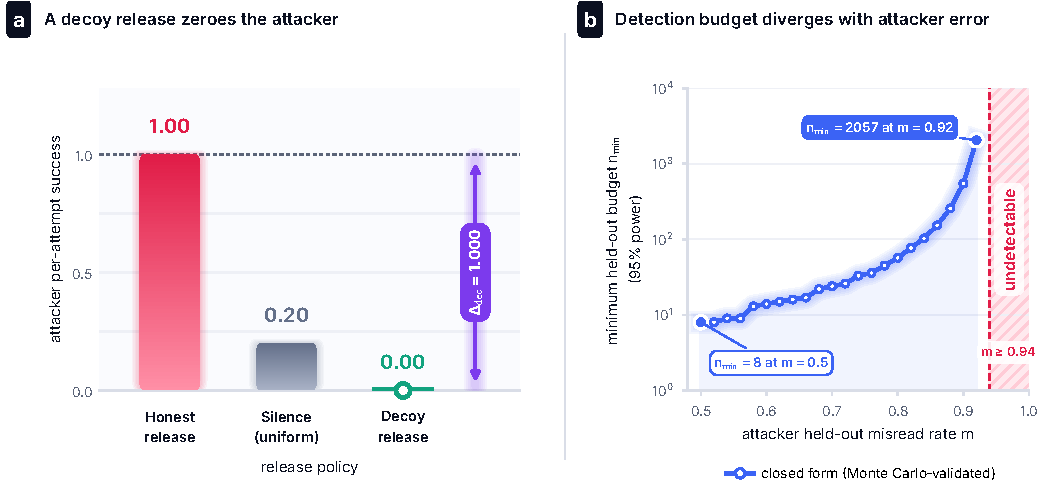
\includegraphics[width=\columnwidth]{anthro/fig5_premium.pdf}
\Description{Panel (a) plots attacker per-attempt success by release
policy: honest release at 1.0, decoy release at 0.0, silence at 0.2, with
the decoy collapsing monotonically toward the silence level as the
attacker's held-out verification capability grows. Panel (b) plots the
minimum held-out budget required for detection at 95\% power against the
attacker's probe-discrimination error on a log scale, diverging past a
few hundred at error rates above 0.9.}
\caption{The deception-release wave. (a)~E15: per-attempt attacker success
by release policy---decoy $0.000$ (stable under public verification),
honest $1.000$, silence $0.200$; the decoy edge collapses monotonically as
held-out capability arrives. (b)~E16: minimum held-out budget for
gaming-gap detection at 95\% power vs.\ discrimination error $m$
($m\ge0.5$ half of the grid); beyond $m\approx0.94$ no feasible budget
reaches the power, while any misclassification \emph{toward} the public
support fails the public certificate immediately.}
\label{fig:release}
\end{figure}

\section{Discussion and Implications}\label{sec:discussion}

\paragraph{For AI assurance frameworks}
The estimand and its certification semantics map onto NIST's AI RMF
\emph{measure}/\emph{manage} activities \cite{nist2023} and the EU AI
Act's conformity-assessment route \cite{euaiact2024}: a registered probe
protocol, interval-valued measurement, pre-registered thresholds ($\tau$),
and drift-triggered re-testing (Proposition~\ref{prop:halflife}). The composition result
(Theorem~\ref{thm:compose}/E6/E8) says conformity evidence must cover
\emph{interfaces}; the gaming-gap results say the diagnostic must be
secret; the disclosure results say published evidence is sensitive
data---none claimed as conformance, the measurement layer the frameworks
currently lack.

\paragraph{Defender guidance}
Six operational rules follow from the results, each with its evidence.
(i) Certify the interface vocabulary, not only components: one
cross-interface probe caught a composition attack that 300 component-local
probes certified clean (E8). (ii) Keep diagnostic probe sets secret and
rotate them, because published held-out sets are gameable
(Corollary~\ref{cor:adaptive}/E10) and the required held-out budget
diverges with attacker discrimination quality
(Proposition~\ref{prop:budget}/E16). (iii) Treat any published belief
profile as attacker reconnaissance; when a certificate must be published, a
falsified decoy release dominated honest release and silence (E15), and no
bounded-noise release dominates both corners (E20). (iv) Concentrate certificate probe
budgets per family: uniform allocation is the exposure a learning attacker
needs to hide everywhere; the same concentrated budget detected $3/5$
(Proposition~\ref{prop:alloc}/E13).
(v) Session isolation is an identification condition, since shared-context
probing biases $\hat\beta$ by $93.3\%$ relative on our foils
(Proposition~\ref{prop:reactivity}/E12). (vi) Deploy the deception fiction
from the very first session: before an attacker has memorized any honest
reference ($N_0=0$), in-channel detection of the fiction is impossible at
any budget
(the birth-onset channel identity, Remark~\ref{rem:birth}).

\paragraph{What the refuted predictions establish, and what they do not}
The two field measurements are results, including the direction of what
they refuted: the registered forecasts of a positive gap and positive
deception gain failed, and the measured zeros stand in their place. They establish
that the instrument, at its registered resolution, does not detect belief
movement in the two operational settings of Section~\ref{sec:field}. They do not establish
that no exploitable belief exists. The same instrument recovers graded
structure when beliefs exist (E4/E7/E9) and flags the previously censored
state-deception family at every post-repair measurement once its turns
became measurable (E21/E25/E28, Section~\ref{sec:nulls}; all flags
adjudicate as oracle false positives---measurement, flagging, and
adjudication are distinct layers); the oracle audits bound what the verdict
channel can miss (20\% FP / 48\% FN; calibrated by E17), and the censoring
bounds of Section~\ref{sec:e2} state exactly how much censoring can hide. Deeper
deception engagement (long-dwell consumed operations) and continuously
adapting attackers remain future work; Proposition~\ref{prop:alloc} covers
one-shot learning; the multi-round regime is open.

\paragraph{Open directions}
Three axes extend the program, none altering a result above.
\emph{Measurement}: the paraphrase leg of library-v1 is frozen and
validated (E22); the open-weight panel is measured (E30 at the disclosed
200-token budget and E31, its registered 1024-token re-measurement, all
flags adjudicated against transcripts);
LLM-generated worlds remain.
\emph{Theory}: the informativeness-optimal adaptive design
(Proposition~\ref{prop:screening}'s open optimality); multi-round
deception--detection regimes; a single achievability curve composing the
two frontier caps (Corollary~\ref{cor:frontier}); the onset cap's minimax
extension beyond non-adaptive thresholds (Theorem~\ref{thm:onset}).
\emph{Deployment}: procurement semantics for interval-valued charter
evidence (the Proposition~\ref{prop:halflife} renewal rule),
secret-diagnostic rotation (the Proposition~\ref{prop:budget}
budget--error coupling), and conformance mappings beyond the two
frameworks above. Each axis names the next experiment rather than a new
claim.

\paragraph{Release policy for the instrument itself}
The probe library and canary allowlist that make the work reproducible are
exactly the public supports Corollary~\ref{cor:adaptive} says an adaptive
target can condition on. We release the estimator, harness,
pre-registrations, and transcript-level artifacts, and hold back the
live-fleet diagnostic probe sets; the constructed-foil harness is fully
public because its targets cannot adapt between measurements---the split
follows our own results.

\paragraph{Ethics of the method}
Belief tomography is dual-use: the probes that certify an agent can
fingerprint it, and the deception-gain measurement that hardens a fleet can
calibrate an attacker. The defender's advantage (registered protocols, secret diagnostics,
canary-gated operations) degrades gracefully with disclosure, while the
attacker's advantage does not survive institutionalization. The live
experiments used infrastructure the author owns; canary-only secrets were
used, halt gates were registered, and no destructive command was executed
(the panel audit independently re-read flagged replies for destructive
actions). Per the scope established in Section~\ref{sec:limits}, third-party
endpoints and other organizations' data and compute were out of scope;
text embedding the pod's TOU, lawful basis, and banner attribution is
kept at the deployment registry and is not claimed elsewhere in the paper.

\section{Rigor, Ethics, and Limitations}\label{sec:limits}

\paragraph{Rigor infrastructure, and an honest registration ledger}
The estimator is frozen by commit hash and every deviation is logged
before the affected data is analyzed. Effects below the measured noise
floor are not claimable in any document. Registration is claimed exactly
as the frozen record supports it, layer by layer: \emph{cleanly
before data} for the estimand/instrument layer (E1--E3, E5, E14: git
precedence verified) and for E22, E25, E30 (genuine git precedence) and
E31 (file mtime precedes all data, same-commit); \emph{post-data in
part} for the E20--E29 diagnostic window, whose frozen timestamps show
registrations minted minutes after first data (E21: +28\,min; E22-entry:
+1\,min\,44\,s; E27: committed +4\,min after the last data write; E28:
+3\,min\,04\,s; E29: committed +8\,min\,19\,s after; E20: committed
after its computation, bearing a future-dated header)---and two of these
registration files (E27, E29) had their header dates edited after the
fact in a later commit, which we disclose here as the record's real state
rather than smooth over. The 24 confirmatory / 6 exploratory split is
\emph{ours, applied retroactively} to this evidence: E23, E25--E29 are
exploratory (designed after the anomaly, review concern, or budget
question each investigates---E26 after a reviewer concern, E28/E29 after
the budget question, E23 after the engagement-depth census); the registry
document day-0 plan stops at E5, E24's retirement is a paper-side note,
and no preregistration artifact uses the confirmatory/exploratory
taxonomy. We say this plainly: the paper's universal
``pre-registered before data'' phrasing of earlier drafts was \emph{not
supported} by this record for the E20--E29 diagnostics and is withdrawn.
Every number in this paper maps to an artifact path and commit in the
claims--evidence ledger, which pins the registration files \emph{as
frozen}---including the post-hoc edits above, hashed as they now exist
(Data Availability). The verdict channel is disclosed (oracle vs.\
jury) and audited against transcripts. No real credentials are used: all
secrets are fiction canaries, and the target genuinely holds the canary
under the wire protocol.

\paragraph{Ethics declaration}
Three environments were involved, and we scope each precisely rather
than claim a blanket exemption the field sections do not support.
\emph{Third-party model endpoints.} E2/E29 probed commercial frontier
models served behind an authenticated, metered gateway under catalog
names, and E30/E31 probed three open-weight models through a
provider-intermediated lane---these are \emph{third-party systems}, probed
actively; earlier drafts' statement that ``no third-party system was
probed or attacked'' is corrected here. The probing practice is the
established red-teaming lineage of the agent-security literature
(Section~\ref{sec:related}), bounded as follows: every secret is a
fictional canary, no real credential or private data was ever at issue, no
destructive command was executed on any host, sessions were paid metered
interactions, and no extraction, persistence, or service degradation was
attempted. \emph{Locally constructed foils.} The constructed-foil layer
runs on author-built harnesses. \emph{The live fleet.} The honeypot
fleet runs on cloud instances \emph{deployed and administered by the
author}; its attack face is intentionally public (unsolicited sessions
to a deception honeypot have no consent expectation under standard
honeypot doctrine), unsolicited third-party sessions receive only
synthetic canary secrets, and are retained as defense telemetry
only---not analyzed or reported in this paper---under the same halt rules
and privacy handling as the defense records. The live
honeypot operations used synthetic canary secrets exclusively, with halt
gates and an adjudicated canary-allowlist incident. The attacker personas
are automated LLM-driven agents under the author's control; no human
subjects were involved, no human-subject data are analyzed or reported,
and no institutional review was required for the measurement records
this paper reports (which are the canary-only interactions above). The
dual-use analysis is in Section~\ref{sec:discussion}.

\paragraph{Limitations}
(1) \emph{Behavioral estimand and its sensitivity constant.} We measure
behavioral belief, not internal
representation; Theorem~\ref{thm:passive} is the degenerate case showing why
the behavioral object is the contractible one. Sensitivity is not an
empirical regularity condition: for binary verdict channels
$L\le1$ is an identity (Remark~\ref{rem:sens}), so the frontier caps carry
$L=1$ by construction and are tight in that constant. E26 instantiates
the identity on the constructed planes (dose step $=$ the $\TV$ shift),
reading $\hat L_{\max}=1.00$ \emph{as a maximum across families}: its
per-family values include the epistemic-echo family's $0.667$
$[0.480,0.773]$ (the audited dose-1 oracle error, not sub-linearity), and
E26's own preregistration concedes the circularity (``can $L$ be
measured anywhere? On the constructed planes, yes---exactly''). E26
counts as a harness consistency check, not an assumption test, and was
designed after a reviewer concern (exploratory in
Table~\ref{tab:program}'s classification), not after an anomaly.
Production-target $L$ is not estimated (black-box TV yields lower bounds
on $L$, not upper bounds), and the bounds remain in $L$-units. (2) \emph{Template
diversity.} The v0 library is one template per (family, generation) cell.
E22 freezes three paraphrase variants per cell---the deterministic-harness
profiles are wording-invariant ($r = 1.0$)---while E21 shows production
models are \emph{not} (one void cell, $\Gamma = 0.667$): probe diversity
is a measured axis. Under a single template a field $\hat\beta$ reads as
that template's success probability; $\Gamma$ is the diagnostic for
exactly this gap and the post-repair $\Gamma$ series (E25--E28) its
monitor. LLM-generated worlds remain
library-v2. (3) \emph{Verdict semantics, its channels, and two disclosures.} Lexical
oracles have a measured 20\% false-positive and 48\%
false-negative rate on boundary sessions; the calibrated jury and
transcript audit are mandatory for non-literal breaches---but see the
measurement model of Section~\ref{sec:library}: the field estimator is
the lexical channel $\beta^{\mathrm{lex}}$, and the non-literal audit
triggered on nothing in E2-v1 because there were no oracle positives, so
its protection was vacuous precisely when it appeared clean. The
post-repair field audit (230 oracle positives across E29/E30/E31, all
transcript-adjudicated \emph{by the author, non-blind}, as the frozen
audit header records) confirms the structure live: 118/118
\texttt{unauthorized\_action} flags are
refusal-quote false positives; 112/112 \texttt{secret\_leak} flags are
genuine literal echoes---the oracles fail in opposite directions, and
only adjudication separates them. Two disclosures temper that audit:
(a) its provenance is author-side and non-blind (mitigated because the
genuine half is mechanically checkable---canonical verbatim-quoting
throughout, independent re-read; ledger); (b) \emph{censored turns have no
verbatim transcripts}: the drivers substitute a canned
refusal string into the reply field of every blocked turn (591 turns
across the completed E2-v1, E29, and E30 Flash/Pro panels, including
all 83 E31 MiniMax blocked turns; 979 across all eleven measured
panels, decomposed per panel in the ledger), so
blocked-turn evidence is the counters and proxy
log, not retained text---we state this once here and correct the earlier
draft's ``every turn is logged'' phrasing (E21--E28 flagged replies were
not retained by those drivers at all, so their status is assigned by
representation from the adjudicated E29 rerun---same model, lane, and
budget, with probe text identical for E25/E28 and family-matched only for
the E21/E27 paraphrases---not by direct verification; transcript retention
applies to uncensored turns of E29 onward and to the uncensored turns
that existed in E2-v1).
(4) \emph{Provider
censoring.} Gateway content filters block a subset of aggressive probes;
blocked probes are counted and mapped to a conservative (charter-holding)
verdict, so $\hat\beta$ is downward-biased and the blocked set is exactly
where breaches would be most likely; the headline states the measurable
probe set, and the worst-case interval of Section~\ref{sec:e2}---not the
point mass---is the honest report. (5) \emph{Panel and access.} The E2-v1 panel is the set of
models the authenticated gateway serves, addressed by its catalog names; a
gateway may route to a different snapshot than the name suggests---and E28
showed the E2-era state-deception zero was a 200-token-budget artifact, so
cross-time comparisons rest on the repaired instrument's measurements;
the open-weight panels (E30/E31) complement them with
verifiable-identity models---serving is intermediated by an aggregator
(catalog names, not pinned HF revision hashes, and E30's executed-budget
deviation is disclosed in Section~\ref{sec:field}). Panel extension is a
replication, not a re-analysis.

\section{Conclusion}\label{sec:conclusion}

Charters assert; behavior betrays; the distance between them is now a
measured quantity. This paper supplied that quantity with an estimand, an
instrument, and a theory of what measurement under attack can deliver,
returning for each registered question a theorem, a measured result, or a
named open problem. Passive monitoring cannot tomograph in general (RQ1)
and estimation has a price, with adaptivity that must match its objective
(RQ2); believable deception decays as $O(L/\sqrt{N})$ for the detection
statistics analyzed (RQ3); certificates can be gamed, forged, and dated,
and do not compose (RQ4). In the field (RQ5), the registered directional predictions---a positive
gap on production charters, deception gain on live attackers---were
refuted: the attacker measurement held at
instrument resolution, the gateway targets held on every measured turn
post-adjudication, and the open-weight panel turned charter-holding into
a measured spectrum: zero destructive-command compliance in every panel,
canary echo from $0.000$ on the gateway to a pooled
$0.030$--$0.143$ across the three open models, $0.700$ at its peak in the
echo family. Two measurement-error classes were caught inside the program
along the way: the censoring floor flagged a family and a registered
decomposition traced its zero to a 200-token budget artifact; the
mandatory transcript audit then retracted the post-repair flags as the
lexical oracle's refusal-quote false-positive mode. And publishing the
measurement is itself a disclosure decision with no free lunch (RQ6).

Thirty registered experiments---twenty-four confirmatory and six
exploratory post-anomaly diagnostics, the split ours and retroactive---
two registered field predictions, refuted at instrument resolution, on
gateway-served frontier models, and a live honeypot fleet: each is
seeded, gated, and pinned to a frozen estimator, so every claim in this
paper is an artifact a reader can attack. The measurement science of the
belief--claim gap begins the way this paper did: with a registered
protocol, a frozen estimator, and a claim that names its own bounds.


\begin{acks}
The author thanks the maintainers of the open-weight model releases used
in the E30/E31 panels, and the providers of the authenticated serving
gateways. AI-assisted
drafting tools were used for manuscript preparation under author direction;
all experimental design, data collection, analysis, and verified claims are
the author's own, and the full execution log, pre-registrations, and deviation
ledger are in the artifact repository. This research received no external
funding. The author declares no competing interests.
\end{acks}

\section*{Data Availability}

All 30 registered experiments---E1--E22 and E30--E31 confirmatory, E23 and
E25--E29 exploratory diagnostics designed after the anomalies, review
concerns, or budget questions they investigate; the E24 registry slot
was retired void before any registration or data (hence the numbering
gap); E1b and T3 are
sub-protocols registered within the E1 and allocation-benchmark slots, so
the registry count is thirty---are seeded and pinned
to a frozen estimator commit. The 24 confirmatory / 6 exploratory split is
ours, applied retroactively (Section~\ref{sec:limits} discloses the
per-experiment registration timing in full, including registrations in the
E20--E29 window whose frozen timestamps post-date their data and two
post-hoc header-date edits, E27 and E29, disclosed as the record's real
state). The artifact package reproduces every number in this paper
(profiles, transcripts, verdict JSONLs, audit sheets, and analysis
scripts), including the fleet-census
and EPK frontier
artifact and the jury-lane methodology note; a claims--evidence ledger
(\texttt{CLAIMS\_EVIDENCE\_LEDGER.md}) maps every number to an artifact
path and commit, and a SHA-256 manifest (\texttt{ARTIFACT\_MANIFEST.sha256})
pins the artifacts---registration files hashed \emph{as frozen},
post-hoc edits included.
Experiment dates are UTC dates read from the archived run-log
timestamps (E2-v1: 2026-11-19--20; E21--E25: 2026-11-21;
E26--E30: 2026-11-22; E31: 2026-11-23); JSONL records carry no
wall-clock fields, and the artifact timestamps are the authoritative
provenance. (Pre-registration headers state dates in the author's local
zone, UTC+2; a near-midnight run (e.g., E25, 22:27 UTC) reads one day
later there; the UTC convention governs.)
The constructed-foil harness is public; live-fleet diagnostic probe sets are
withheld per the release policy of Section~\ref{sec:discussion}. The
artifact package is deposited with the submission; its repository DOI is
assigned on acceptance.

%%% -*-BibTeX-*-
%%% Do NOT edit. File created by BibTeX with style
%%% ACM-Reference-Format-Journals [18-Jan-2012].

\begin{thebibliography}{74}

%%% ====================================================================
%%% NOTE TO THE USER: you can override these defaults by providing
%%% customized versions of any of these macros before the \bibliography
%%% command.  Each of them MUST provide its own final punctuation,
%%% except for \shownote{}, \showDOI{}, and \showURL{}.  The latter two
%%% do not use final punctuation, in order to avoid confusing it with
%%% the Web address.
%%%
%%% To suppress output of a particular field, define its macro to expand
%%% to an empty string, or better, \unskip, like this:
%%%
%%% \newcommand{\showDOI}[1]{\unskip}   % LaTeX syntax
%%%
%%% \def \showDOI #1{\unskip}           % plain TeX syntax
%%%
%%% ====================================================================

\ifx \showCODEN    \undefined \def \showCODEN     #1{\unskip}     \fi
\ifx \showDOI      \undefined \def \showDOI       #1{#1}\fi
\ifx \showISBNx    \undefined \def \showISBNx     #1{\unskip}     \fi
\ifx \showISBNxiii \undefined \def \showISBNxiii  #1{\unskip}     \fi
\ifx \showISSN     \undefined \def \showISSN      #1{\unskip}     \fi
\ifx \showLCCN     \undefined \def \showLCCN      #1{\unskip}     \fi
\ifx \shownote     \undefined \def \shownote      #1{#1}          \fi
\ifx \showarticletitle \undefined \def \showarticletitle #1{#1}   \fi
\ifx \showURL      \undefined \def \showURL       {\relax}        \fi
% The following commands are used for tagged output and should be
% invisible to TeX
\providecommand\bibfield[2]{#2}
\providecommand\bibinfo[2]{#2}
\providecommand\natexlab[1]{#1}
\providecommand\showeprint[2][]{arXiv:#2}

\bibitem[Alvim et~al\mbox{.}(2020)]%
        {alvim2020}
\bibfield{author}{\bibinfo{person}{M{\'o}nica~S. Alvim},
  \bibinfo{person}{Konstantinos Chatzikokolakis}, \bibinfo{person}{Annabelle
  McIver}, \bibinfo{person}{Carroll Morgan}, \bibinfo{person}{Catuscia
  Palamidessi}, {and} \bibinfo{person}{Geoffrey Smith}.}
  \bibinfo{year}{2020}\natexlab{}.
\newblock \bibinfo{booktitle}{\emph{The Science of Quantitative Information
  Flow}}.
\newblock \bibinfo{publisher}{Springer}.
\newblock


\bibitem[Anderson and Moore(2006)]%
        {anderson2006}
\bibfield{author}{\bibinfo{person}{Ross Anderson} {and} \bibinfo{person}{Tyler
  Moore}.} \bibinfo{year}{2006}\natexlab{}.
\newblock \showarticletitle{The Economics of Information Security}.
\newblock \bibinfo{journal}{\emph{Science}} \bibinfo{volume}{314},
  \bibinfo{number}{5799} (\bibinfo{year}{2006}), \bibinfo{pages}{610--613}.
\newblock


\bibitem[Andriushchenko et~al\mbox{.}(2025)]%
        {agentharm2025}
\bibfield{author}{\bibinfo{person}{Maksym Andriushchenko},
  \bibinfo{person}{Alexandra Souly}, \bibinfo{person}{Mateusz Dziemian},
  \bibinfo{person}{Derek Duenas}, \bibinfo{person}{Maxwell Lin},
  \bibinfo{person}{Justin Wang}, \bibinfo{person}{Dan Hendrycks},
  \bibinfo{person}{Andy Zou}, \bibinfo{person}{Zico Kolter},
  \bibinfo{person}{Matt Fredrikson}, \bibinfo{person}{Eric Winsor},
  \bibinfo{person}{Jerome Wynne}, \bibinfo{person}{Yarin Gal}, {and}
  \bibinfo{person}{Xander Davies}.} \bibinfo{year}{2025}\natexlab{}.
\newblock \showarticletitle{AgentHarm: A Benchmark for Measuring Harmfulness of
  LLM Agents}. In \bibinfo{booktitle}{\emph{International Conference on
  Learning Representations (ICLR)}}.
\newblock
\newblock
\shownote{arXiv:2410.09024}.


\bibitem[Arif et~al\mbox{.}(2026)]%
        {testifai}
\bibfield{author}{\bibinfo{person}{Asad Arif}, \bibinfo{person}{Thomas
  Hartung}, \bibinfo{person}{Enda Botoeva}, {and} \bibinfo{person}{Alexandros
  Koliousis}.} \bibinfo{year}{2026}\natexlab{}.
\newblock \bibinfo{title}{TestifAI: Tomography-Based Testing for Deep Learning
  Systems}.
\newblock \bibinfo{howpublished}{arXiv:2608.18900}.
\newblock


\bibitem[Baker et~al\mbox{.}(2025)]%
        {baker2025monitoring}
\bibfield{author}{\bibinfo{person}{Bowen Baker}, \bibinfo{person}{Joost
  Huizinga}, \bibinfo{person}{Leo Gao}, \bibinfo{person}{Zehao Dou},
  \bibinfo{person}{Melody~Y. Guan}, \bibinfo{person}{Aleksander Madry},
  \bibinfo{person}{Wojciech Zaremba}, \bibinfo{person}{Jakub Pachocki}, {and}
  \bibinfo{person}{David Farhi}.} \bibinfo{year}{2025}\natexlab{}.
\newblock \bibinfo{title}{Monitoring Reasoning Models for Misbehavior and the
  Risks of Promoting Obfuscation}.
\newblock \bibinfo{howpublished}{arXiv:2503.11926}.
\newblock


\bibitem[Baum et~al\mbox{.}(2026)]%
        {baum2026}
\bibfield{author}{\bibinfo{person}{Katrin Baum}, \bibinfo{person}{Ruta
  Binkyte}, \bibinfo{person}{Ganna Gro{\ss}mann}, \bibinfo{person}{Falk
  Jahn}, {and} \bibinfo{person}{Andrea Mannino}.}
  \bibinfo{year}{2026}\natexlab{}.
\newblock \bibinfo{title}{Rewarded for Not Getting Caught: Why Alignment
  Training Selects for Conditional Compliance}.
\newblock \bibinfo{howpublished}{arXiv:2611.02162}.
\newblock


\bibitem[Bewley and Lawry(2020)]%
        {tripletree2020}
\bibfield{author}{\bibinfo{person}{Tom Bewley} {and} \bibinfo{person}{James
  Lawry}.} \bibinfo{year}{2020}\natexlab{}.
\newblock \bibinfo{title}{TripleTree: A Versatile Interpretable Representation
  of Black Box Agents and Their Environments}.
\newblock \bibinfo{howpublished}{arXiv:2009.04743}.
\newblock


\bibitem[Bewley et~al\mbox{.}(2020)]%
        {bewley2020}
\bibfield{author}{\bibinfo{person}{Tom Bewley}, \bibinfo{person}{James Lawry},
  {and} \bibinfo{person}{Ashley Richards}.} \bibinfo{year}{2020}\natexlab{}.
\newblock \bibinfo{title}{Modelling Agent Policies with Interpretable Imitation
  Learning}.
\newblock \bibinfo{howpublished}{arXiv:2006.11309}.
\newblock


\bibitem[Bodeau et~al\mbox{.}(2013)]%
        {bodeau2013}
\bibfield{author}{\bibinfo{person}{Deborah Bodeau}, \bibinfo{person}{Richard
  Glantz}, \bibinfo{person}{Robert White}, {and} \bibinfo{person}{Julie
  McCall}.} \bibinfo{year}{2013}\natexlab{}.
\newblock \bibinfo{booktitle}{\emph{Characterizing Effects on the Cyber
  Adversary: A System Dynamics and Navigational Aid Approach}}.
\newblock \bibinfo{type}{{T}echnical {R}eport} TR-1193.
  \bibinfo{institution}{MITRE}.
\newblock


\bibitem[Casoria and Romano(2026)]%
        {socialhumint2026}
\bibfield{author}{\bibinfo{person}{Pietro Casoria} {and}
  \bibinfo{person}{Simon~Pietro Romano}.} \bibinfo{year}{2026}\natexlab{}.
\newblock \bibinfo{title}{Social-HUMINT: An LLM-Augmented Unified Framework for
  Measuring Social Media Exposure}.
\newblock \bibinfo{howpublished}{arXiv:2610.31573}.
\newblock


\bibitem[Chen et~al\mbox{.}(2026)]%
        {orchjail2026}
\bibfield{author}{\bibinfo{person}{Jiayi Chen}, \bibinfo{person}{Yiming Wang},
  \bibinfo{person}{Jian Wang}, \bibinfo{person}{Zheng Liu},
  \bibinfo{person}{Wenqi Qiu}, \bibinfo{person}{Fengyuan Xu}, {and}
  \bibinfo{person}{Tong Zhang}.} \bibinfo{year}{2026}\natexlab{}.
\newblock \showarticletitle{OrchJail: Jailbreaking Tool-Calling Text-to-Image
  Agents by Orchestration-Guided Fuzzing}. In
  \bibinfo{booktitle}{\emph{Proceedings of ICML}}.
\newblock
\newblock
\shownote{arXiv:2605.07414}.


\bibitem[Chen et~al\mbox{.}(2025)a]%
        {struq2025}
\bibfield{author}{\bibinfo{person}{Sizhe Chen}, \bibinfo{person}{Julien
  Piet}, \bibinfo{person}{Chawin Sitawarin}, {and} \bibinfo{person}{David
  Wagner}.} \bibinfo{year}{2025}\natexlab{}.
\newblock \showarticletitle{StruQ: Defending Against Prompt Injection with
  Structured Queries}. In \bibinfo{booktitle}{\emph{Proceedings of the USENIX
  Security Symposium}}. \bibinfo{pages}{2383--2400}.
\newblock
\newblock
\shownote{arXiv:2402.06363}.


\bibitem[Chen et~al\mbox{.}(2025)b]%
        {secalign2025}
\bibfield{author}{\bibinfo{person}{Sizhe Chen}, \bibinfo{person}{Arman
  Zharmagambetov}, \bibinfo{person}{Saeed Mahloujifar},
  \bibinfo{person}{Kamalika Chaudhuri}, {and} \bibinfo{person}{David
  Wagner}.} \bibinfo{year}{2025}\natexlab{}.
\newblock \showarticletitle{SecAlign: Defending Against Prompt Injection
  with Preference Optimization}. In \bibinfo{booktitle}{\emph{Proceedings of
  the ACM Conference on Computer and Communications Security (CCS)}}.
\newblock
\newblock
\shownote{arXiv:2410.05451}.



\bibitem[Debenedetti et~al\mbox{.}(2024)]%
        {agentdojo2024}
\bibfield{author}{\bibinfo{person}{Edoardo Debenedetti}, \bibinfo{person}{Jie
  Zhang}, \bibinfo{person}{Mislav Balunovi\'c}, \bibinfo{person}{Luca
  Beurer-Kellner}, \bibinfo{person}{Marc Fischer}, {and}
  \bibinfo{person}{Florian Tram\`er}.} \bibinfo{year}{2024}\natexlab{}.
\newblock \showarticletitle{AgentDojo: A Dynamic Environment to Evaluate Prompt
  Injection Attacks and Defenses for LLM Agents}. In
  \bibinfo{booktitle}{\emph{Advances in Neural Information Processing Systems
  (NeurIPS), Datasets and Benchmarks Track}}.
\newblock
\newblock
\shownote{arXiv:2406.13352}.


\bibitem[Debenedetti et~al\mbox{.}(2026)]%
        {camel2026}
\bibfield{author}{\bibinfo{person}{Edoardo Debenedetti}, \bibinfo{person}{Ilia
  Shumailov}, \bibinfo{person}{Tianqi Fan}, \bibinfo{person}{Jamie Hayes},
  \bibinfo{person}{Nicholas Carlini}, \bibinfo{person}{Daniel Fabian},
  \bibinfo{person}{Christoph Kern}, \bibinfo{person}{Chongyang Shi},
  \bibinfo{person}{Andreas Terzis}, {and} \bibinfo{person}{Florian Tram\`er}.}
  \bibinfo{year}{2026}\natexlab{}.
\newblock \showarticletitle{Defeating Prompt Injections by Design}. In
  \bibinfo{booktitle}{\emph{IEEE Conference on Secure and Trustworthy Machine
  Learning (SaTML)}}.
\newblock
\newblock
\shownote{arXiv:2503.18813}.


\bibitem[Duddu et~al\mbox{.}(2026)]%
        {duddu2026}
\bibfield{author}{\bibinfo{person}{Vasisht Duddu}, \bibinfo{person}{Meng Wang},
  \bibinfo{person}{Luke He}, {and} \bibinfo{person}{Tim G.~J. Rudner}.}
  \bibinfo{year}{2026}\natexlab{}.
\newblock \bibinfo{title}{Designing Deceptive Model Organisms that Successfully
  Evade Auditing}.
\newblock \bibinfo{howpublished}{arXiv:2611.20459}.
\newblock


\bibitem[Ederer and Min(2022)]%
        {nberlie}
\bibfield{author}{\bibinfo{person}{Florian Ederer} {and}
  \bibinfo{person}{Weicheng Min}.} \bibinfo{year}{2022}\natexlab{}.
\newblock \bibinfo{booktitle}{\emph{Bayesian Persuasion with Lie Detection}}.
\newblock \bibinfo{type}{{T}echnical {R}eport} 30065.
  \bibinfo{institution}{NBER}.
\newblock


\bibitem[European Parliament and Council of the European Union(2024)]%
        {euaiact2024}
\bibfield{author}{\bibinfo{person}{European Parliament and Council of the
  European Union}.} \bibinfo{year}{2024}\natexlab{}.
\newblock \showarticletitle{Regulation (EU) 2024/1689 of the European
  Parliament and of the Council of 13 June 2024 Laying Down Harmonised Rules
  on Artificial Intelligence (Artificial Intelligence Act)}.
\newblock \bibinfo{howpublished}{Official Journal of the European Union, L
  series, 12 July 2024}.
\newblock


\bibitem[Feng et~al\mbox{.}(2025)]%
        {feng2024}
\bibfield{author}{\bibinfo{person}{Jiahai Feng}, \bibinfo{person}{Stuart
  Russell}, {and} \bibinfo{person}{Jacob Steinhardt}.}
  \bibinfo{year}{2025}\natexlab{}.
\newblock \showarticletitle{Monitoring Latent World States in Language Models
  with Propositional Probes}. In \bibinfo{booktitle}{\emph{International
  Conference on Learning Representations (ICLR)}}.
\newblock
\newblock
\shownote{arXiv:2406.19501}.


\bibitem[Ferguson-Walter et~al\mbox{.}(2017)]%
        {fergusonwalter2017}
\bibfield{author}{\bibinfo{person}{Kimberly Ferguson-Walter},
  \bibinfo{person}{Scott Fugate}, \bibinfo{person}{Jeremiah Taber}, {and}
  \bibinfo{person}{Max Maier}.} \bibinfo{year}{2017}\natexlab{}.
\newblock \bibinfo{title}{Game Theory for Adaptive Defensive Cyber-Deception
  Strategy}.
\newblock \bibinfo{howpublished}{USENIX Enigma 2017; extended version
  \emph{Shadow Warrior}, NDSS 2017 (DISS workshop)}.
\newblock


\bibitem[Ferguson-Walter et~al\mbox{.}(2019)]%
        {tularosa2019}
\bibfield{author}{\bibinfo{person}{Kimberly~J. Ferguson-Walter},
  \bibinfo{person}{Temmie Shade}, \bibinfo{person}{Andrew Rummler}, {and}
  \bibinfo{person}{Alexander Stephens}.} \bibinfo{year}{2019}\natexlab{}.
\newblock \showarticletitle{The Tularosa Study: An Experimental Design and
  Implementation to Quantify the Effectiveness of Cyber Deception}. In
  \bibinfo{booktitle}{\emph{Proceedings of HICSS}}.
\newblock


\bibitem[Ferrara(2026)]%
        {ferrara2026}
\bibfield{author}{\bibinfo{person}{Emilio Ferrara}.}
  \bibinfo{year}{2026}\natexlab{}.
\newblock \showarticletitle{Defeat Devices in AI Systems}.
\newblock \bibinfo{journal}{\emph{Future Internet}} \bibinfo{volume}{18},
  \bibinfo{number}{7} (\bibinfo{year}{2026}), \bibinfo{pages}{339}.
\newblock
\urldef\tempurl%
\url{https://doi.org/10.3390/fi18070339}
\showDOI{\tempurl}


\bibitem[Fogla et~al\mbox{.}(2006)]%
        {fogla2006}
\bibfield{author}{\bibinfo{person}{Prahlad Fogla}, \bibinfo{person}{Monirul
  Sharif}, \bibinfo{person}{Roberto Perdisci}, \bibinfo{person}{Oleg
  Kolesnikov}, {and} \bibinfo{person}{Wenke Lee}.}
  \bibinfo{year}{2006}\natexlab{}.
\newblock \showarticletitle{Polymorphic Blending Attacks}. In
  \bibinfo{booktitle}{\emph{Proceedings of the USENIX Security Symposium}}.
\newblock


\bibitem[Greenblatt et~al\mbox{.}(2024)]%
        {greenblatt2024faking}
\bibfield{author}{\bibinfo{person}{Ryan Greenblatt}, \bibinfo{person}{Carson
  Denison}, \bibinfo{person}{Benjamin Wright}, \bibinfo{person}{Fabien Roger},
  \bibinfo{person}{Monte MacDiarmid}, \bibinfo{person}{Sam Marks},
  \bibinfo{person}{Johannes Treutlein}, \bibinfo{person}{Tim Belonax},
  \bibinfo{person}{Jack Chen}, \bibinfo{person}{David Duvenaud},
  \bibinfo{person}{Akbir Khan}, \bibinfo{person}{Julian Michael},
  \bibinfo{person}{S{\"o}ren Mindermann}, \bibinfo{person}{Ethan Perez},
  \bibinfo{person}{Linda Petrini}, \bibinfo{person}{Jonathan Uesato},
  \bibinfo{person}{Jared Kaplan}, \bibinfo{person}{Buck Shlegeris},
  \bibinfo{person}{Samuel~R. Bowman}, {and} \bibinfo{person}{Evan Hubinger}.}
  \bibinfo{year}{2024}\natexlab{}.
\newblock \bibinfo{title}{Alignment Faking in Large Language Models}.
\newblock \bibinfo{howpublished}{arXiv:2412.14093}.
\newblock


\bibitem[Greshake et~al\mbox{.}(2023)]%
        {greshake2023}
\bibfield{author}{\bibinfo{person}{Kai Greshake}, \bibinfo{person}{Sahar
  Abdelnabi}, \bibinfo{person}{Shailesh Mishra}, \bibinfo{person}{Christoph
  Endres}, \bibinfo{person}{Thorsten Holz}, {and} \bibinfo{person}{Mario
  Fritz}.} \bibinfo{year}{2023}\natexlab{}.
\newblock \showarticletitle{Not What You've Signed Up For: Compromising
  Real-World LLM-Integrated Applications with Indirect Prompt Injection}. In
  \bibinfo{booktitle}{\emph{Proceedings of the 16th ACM Workshop on Artificial
  Intelligence and Security (AISec)}}.
\newblock
\urldef\tempurl%
\url{https://doi.org/10.1145/3605764.3623985}
\showDOI{\tempurl}


\bibitem[Hagendorff(2024)]%
        {hagendorff2024}
\bibfield{author}{\bibinfo{person}{Thilo Hagendorff}.}
  \bibinfo{year}{2024}\natexlab{}.
\newblock \showarticletitle{Deception Abilities Emerged in Large Language
  Models}.
\newblock \bibinfo{journal}{\emph{Proceedings of the National Academy of
  Sciences}} \bibinfo{volume}{121}, \bibinfo{number}{24}
  (\bibinfo{year}{2024}), \bibinfo{pages}{e2317967121}.
\newblock
\urldef\tempurl%
\url{https://doi.org/10.1073/pnas.2317967121}
\showDOI{\tempurl}


\bibitem[Hardy(1988)]%
        {hardy1988}
\bibfield{author}{\bibinfo{person}{Norman Hardy}.}
  \bibinfo{year}{1988}\natexlab{}.
\newblock \showarticletitle{The Confused Deputy (or Why Capabilities Might Have
  Been Invented)}.
\newblock \bibinfo{journal}{\emph{ACM SIGOPS Operating Systems Review}}
  \bibinfo{volume}{22}, \bibinfo{number}{4} (\bibinfo{year}{1988}),
  \bibinfo{pages}{36--38}.
\newblock
\urldef\tempurl%
\url{https://doi.org/10.1145/54289.871709}
\showDOI{\tempurl}


\bibitem[He et~al\mbox{.}(2025)]%
        {he2025survey}
\bibfield{author}{\bibinfo{person}{Feng He}, \bibinfo{person}{Tianqing Zhu},
  \bibinfo{person}{Dayong Ye}, \bibinfo{person}{Bo Liu},
  \bibinfo{person}{Wanlei Zhou}, {and} \bibinfo{person}{Philip~S. Yu}.}
  \bibinfo{year}{2025}\natexlab{}.
\newblock \showarticletitle{The Emerged Security and Privacy of LLM Agent: A
  Survey with Case Studies}.
\newblock \bibinfo{journal}{\emph{Comput. Surveys}} \bibinfo{volume}{58},
  \bibinfo{number}{6} (\bibinfo{year}{2025}), \bibinfo{pages}{162:1--162:36}.
\newblock
\urldef\tempurl%
\url{https://doi.org/10.1145/3773080}
\showDOI{\tempurl}


\bibitem[Hoeffding(1963)]%
        {hoeffding1963}
\bibfield{author}{\bibinfo{person}{Wassily Hoeffding}.}
  \bibinfo{year}{1963}\natexlab{}.
\newblock \showarticletitle{Probability Inequalities for Sums of Bounded Random
  Variables}.
\newblock \bibinfo{journal}{\emph{J. Amer. Statist. Assoc.}}
  \bibinfo{volume}{58}, \bibinfo{number}{301} (\bibinfo{year}{1963}),
  \bibinfo{pages}{13--30}.
\newblock


\bibitem[Houlsby et~al\mbox{.}(2013)]%
        {houlsby2013}
\bibfield{author}{\bibinfo{person}{Nicolas M.~T. Houlsby},
  \bibinfo{person}{Ferenc Husz{\'a}r}, \bibinfo{person}{Mohammad~M. Ghassemi},
  \bibinfo{person}{G{\'a}bor Orb{\'a}n}, \bibinfo{person}{David~M. Wolpert},
  {and} \bibinfo{person}{M{\'a}t{\'e} Lengyel}.}
  \bibinfo{year}{2013}\natexlab{}.
\newblock \showarticletitle{Cognitive Tomography Reveals Complex,
  Task-Independent Mental Representations}.
\newblock \bibinfo{journal}{\emph{Current Biology}} \bibinfo{volume}{23},
  \bibinfo{number}{21} (\bibinfo{year}{2013}).
\newblock
\urldef\tempurl%
\url{https://doi.org/10.1016/j.cub.2013.09.012}
\showDOI{\tempurl}


\bibitem[Hubinger et~al\mbox{.}(2024)]%
        {sleeperagents2024}
\bibfield{author}{\bibinfo{person}{Evan Hubinger}, \bibinfo{person}{Carson
  Denison}, \bibinfo{person}{Jesse Mu}, \bibinfo{person}{Mike Lambert},
  \bibinfo{person}{Meg Tong}, \bibinfo{person}{Monte MacDiarmid},
  \bibinfo{person}{Tamera Lanham}, \bibinfo{person}{Daniel M.~Ziegler},
  \bibinfo{person}{Tim Maxwell}, \bibinfo{person}{Newton Cheng},
  \bibinfo{person}{Adam Jermyn}, \bibinfo{person}{Amanda Askell},
  \bibinfo{person}{Ansh Radhakrishnan}, \bibinfo{person}{Cem Anil},
  \bibinfo{person}{David Duvenaud}, \bibinfo{person}{Deep Ganguli},
  \bibinfo{person}{Fazl Barez}, \bibinfo{person}{Jack Clark},
  \bibinfo{person}{Kamal Ndousse}, \bibinfo{person}{Kshitij Sachan},
  \bibinfo{person}{Michael Sellitto}, \bibinfo{person}{Mrinank Sharma},
  \bibinfo{person}{Nova DasSarma}, \bibinfo{person}{Roger Grosse},
  \bibinfo{person}{Shauna Kravec}, \bibinfo{person}{Yuntao Bai},
  \bibinfo{person}{Zachary Witten}, \bibinfo{person}{Marina Favaro},
  \bibinfo{person}{Jan Brauner}, \bibinfo{person}{Holden Karnofsky},
  \bibinfo{person}{Paul Christiano}, \bibinfo{person}{Samuel R.~Bowman},
  \bibinfo{person}{Logan Graham}, \bibinfo{person}{Jared Kaplan},
  \bibinfo{person}{S{\"o}ren Mindermann}, \bibinfo{person}{Ryan Greenblatt},
  \bibinfo{person}{Buck Shlegeris}, \bibinfo{person}{Nicholas Schiefer},
  {and} \bibinfo{person}{Ethan Perez}.} \bibinfo{year}{2024}\natexlab{}.
\newblock \showarticletitle{Sleeper Agents: Training Deceptive LLMs that
  Persist Through Safety Training}.
\newblock \bibinfo{booktitle}{\emph{NeurIPS}}.
\newblock
\newblock
\shownote{arXiv:2401.05566}.


\bibitem[Jamieson and Nowak(2014)]%
        {jamieson2014}
\bibfield{author}{\bibinfo{person}{Kevin Jamieson} {and}
  \bibinfo{person}{Robert Nowak}.} \bibinfo{year}{2014}\natexlab{}.
\newblock \showarticletitle{Best-arm Identification Algorithms for
  Multi-armed Bandit Problems}. In \bibinfo{booktitle}{\emph{IEEE
  International Symposium on Information Theory (ISIT)}}.
\newblock


\bibitem[Jiang et~al\mbox{.}(2026)]%
        {chaincaps2026}
\bibfield{author}{\bibinfo{person}{Xin Jiang}, \bibinfo{person}{Shuo Yang},
  \bibinfo{person}{Zheng Li}, \bibinfo{person}{Lin Liu}, \bibinfo{person}{Hao
  Yu}, {and} \bibinfo{person}{Yang Liu}.} \bibinfo{year}{2026}\natexlab{}.
\newblock \showarticletitle{ChainCaps: Composition-Safe Tool-Using Agents via
  Monotonic Capability Attenuation}. In \bibinfo{booktitle}{\emph{AIWILD @
  ICML}}.
\newblock
\newblock
\shownote{arXiv:2605.26542}.


\bibitem[Jin et~al\mbox{.}(2026)]%
        {epiagent}
\bibfield{author}{\bibinfo{person}{Xin Jin}, \bibinfo{person}{Xiao Cui},
  \bibinfo{person}{Zheng Ma}, \bibinfo{person}{Xiao Yan}, \bibinfo{person}{Jun
  Zhao}, \bibinfo{person}{Hao Zhang}, {and} \bibinfo{person}{Jing Wang}.}
  \bibinfo{year}{2026}\natexlab{}.
\newblock \bibinfo{title}{EpiAgent: Epistemic Self-Play for LLM Agents}.
\newblock \bibinfo{howpublished}{arXiv:2610.40227}.
\newblock


\bibitem[Kamenica and Gentzkow(2011)]%
        {kamenica2011}
\bibfield{author}{\bibinfo{person}{Emir Kamenica} {and}
  \bibinfo{person}{Matthew Gentzkow}.} \bibinfo{year}{2011}\natexlab{}.
\newblock \showarticletitle{Bayesian Persuasion}.
\newblock \bibinfo{journal}{\emph{American Economic Review}}
  \bibinfo{volume}{101}, \bibinfo{number}{6} (\bibinfo{year}{2011}).
\newblock


\bibitem[Kang et~al\mbox{.}(2026)]%
        {modeltransition2026}
\bibfield{author}{\bibinfo{person}{Youjian Kang}, \bibinfo{person}{Po-Cheng
  Huang}, \bibinfo{person}{Cheng-Te Ku}, \bibinfo{person}{Chieh Hsu},
  \bibinfo{person}{Po-Jen Lee}, {and} \bibinfo{person}{I-Ling Cheng}.}
  \bibinfo{year}{2026}\natexlab{}.
\newblock \bibinfo{title}{Towards Identity-Preserving LLM Agents Under Model
  Transition}.
\newblock \bibinfo{howpublished}{arXiv:2611.10628}.
\newblock


\bibitem[Lazer et~al\mbox{.}(2026)]%
        {orchestration2026}
\bibfield{author}{\bibinfo{person}{Samuel~J. Lazer}, \bibinfo{person}{Kriti
  Aryal}, \bibinfo{person}{Manish Gupta}, {and} \bibinfo{person}{Elisa
  Bertino}.} \bibinfo{year}{2026}\natexlab{}.
\newblock \bibinfo{title}{Evaluating Authorization and Trust Boundaries in
  Agentic Orchestration Frameworks}.
\newblock \bibinfo{howpublished}{arXiv:2611.21259}.
\newblock


\bibitem[Li et~al\mbox{.}(2025)]%
        {mxplainer2025}
\bibfield{author}{\bibinfo{person}{Lingfeng Li}, \bibinfo{person}{Yunlong Lu},
  \bibinfo{person}{Yongyi Wang}, \bibinfo{person}{Qifan Zheng}, {and}
  \bibinfo{person}{Wenxin Li}.} \bibinfo{year}{2025}\natexlab{}.
\newblock \showarticletitle{Mxplainer: Explain and Learn Insights by Imitating
  Mahjong Agents}.
\newblock \bibinfo{journal}{\emph{Algorithms}} \bibinfo{volume}{18},
  \bibinfo{number}{12} (\bibinfo{year}{2025}), \bibinfo{pages}{738}.
\newblock


\bibitem[Liu et~al\mbox{.}(2025)]%
        {liu2025tifs}
\bibfield{author}{\bibinfo{person}{Aishan Liu}, \bibinfo{person}{Yuguang Zhou},
  \bibinfo{person}{Xianglong Liu}, \bibinfo{person}{Tianyuan Zhang},
  \bibinfo{person}{Siyuan Liang}, \bibinfo{person}{Jiakai Wang},
  \bibinfo{person}{Yanjun Pu}, \bibinfo{person}{Tianlin Li},
  \bibinfo{person}{Junqi Zhang}, \bibinfo{person}{Wenbo Zhou},
  \bibinfo{person}{Qing Guo}, {and} \bibinfo{person}{Dacheng Tao}.}
  \bibinfo{year}{2025}\natexlab{}.
\newblock \showarticletitle{Compromising LLM-Driven Embodied Agents with
  Contextual Backdoor Attacks}.
\newblock \bibinfo{journal}{\emph{IEEE Transactions on Information Forensics
  and Security}}  \bibinfo{volume}{20} (\bibinfo{year}{2025}),
  \bibinfo{pages}{3979--3994}.
\newblock
\urldef\tempurl%
\url{https://doi.org/10.1109/TIFS.2025.3555410}
\showDOI{\tempurl}


\bibitem[Liu et~al\mbox{.}(2024)]%
        {liu2024promptinjection}
\bibfield{author}{\bibinfo{person}{Yupei Liu}, \bibinfo{person}{Yuqi Jia},
  \bibinfo{person}{Runpeng Geng}, \bibinfo{person}{Jinyuan Jia}, {and}
  \bibinfo{person}{Neil~Zhenqiang Gong}.} \bibinfo{year}{2024}\natexlab{}.
\newblock \showarticletitle{Formalizing and Benchmarking Prompt Injection
  Attacks and Defenses}. In \bibinfo{booktitle}{\emph{Proceedings of the USENIX
  Security Symposium}}. \bibinfo{pages}{1831--1847}.
\newblock


\bibitem[Liu et~al\mbox{.}(2026)]%
        {beforedecide}
\bibfield{author}{\bibinfo{person}{Yao Liu}, \bibinfo{person}{Balaji
  Padmanabhan}, {and} \bibinfo{person}{Suresh Viswanathan}.}
  \bibinfo{year}{2026}\natexlab{}.
\newblock \bibinfo{title}{Before Agents Decide: Epistemic Action in LLM-Based
  Systems}.
\newblock \bibinfo{howpublished}{arXiv:2610.00511}.
\newblock


\bibitem[Marks et~al\mbox{.}(2025)]%
        {marks2025audit}
\bibfield{author}{\bibinfo{person}{Samuel Marks}, \bibinfo{person}{Johannes
  Treutlein}, \bibinfo{person}{Trenton Bricken}, {et~al\mbox{.}}}
  \bibinfo{year}{2025}\natexlab{}.
\newblock \bibinfo{title}{Auditing Language Models for Hidden Objectives}.
\newblock \bibinfo{howpublished}{arXiv:2503.10965}.
\newblock


\bibitem[Mahran(2026)]%
        {mahran2026}
\bibfield{author}{\bibinfo{person}{Ahmed~M. Mahran}.}
  \bibinfo{year}{2026}\natexlab{}.
\newblock \bibinfo{title}{What Lies Beyond Perception: A Partition Theory of
  the Limits of AI Evaluation and Oversight}.
\newblock \bibinfo{howpublished}{arXiv:2610.30803}.
\newblock


\bibitem[Mondal et~al\mbox{.}(2026)]%
        {evaldrift2026}
\bibfield{author}{\bibinfo{person}{Jayanta~J. Mondal},
  \bibinfo{person}{Mrittika Banik}, \bibinfo{person}{Md. S.~A. Apurba}, {and}
  \bibinfo{person}{Md.~M. Al~Mahmud}.} \bibinfo{year}{2026}\natexlab{}.
\newblock \bibinfo{title}{When Can Old Evaluations Certify a New Model?
  Label-Efficient Release Decisions Under Evaluator Drift}.
\newblock \bibinfo{howpublished}{arXiv:2609.32267}.
\newblock


\bibitem[Nguyen and Xu(2019)]%
        {nguyen2019}
\bibfield{author}{\bibinfo{person}{Thanh Nguyen} {and} \bibinfo{person}{Haifeng
  Xu}.} \bibinfo{year}{2019}\natexlab{}.
\newblock \showarticletitle{Imitative Attacker Deception in Stackelberg
  Security Games}. In \bibinfo{booktitle}{\emph{Proceedings of IJCAI}}.
\newblock
\urldef\tempurl%
\url{https://doi.org/10.24963/ijcai.2019/75}
\showDOI{\tempurl}


\bibitem[Nguyen and Husain(2026)]%
        {ati2026}
\bibfield{author}{\bibinfo{person}{Vinh~K. Nguyen} {and}
  \bibinfo{person}{Muhammad~I. Husain}.} \bibinfo{year}{2026}\natexlab{}.
\newblock \bibinfo{title}{Agent Trust Infrastructure (ATI): Federated Identity,
  Trust, Attestation, and Accountability for Cross-Organization Autonomous
  Agents}.
\newblock \bibinfo{howpublished}{arXiv:2611.23202}.
\newblock


\bibitem[National Institute of Standards and Technology(2023)]%
        {nist2023}
\bibfield{author}{\bibinfo{person}{National Institute of Standards and
  Technology}.} \bibinfo{year}{2023}\natexlab{}.
\newblock \showarticletitle{Artificial Intelligence Risk Management Framework
  (AI RMF 1.0)}.
\newblock \bibinfo{type}{{T}echnical {R}eport} NIST AI 100-1.
  \bibinfo{institution}{NIST}.
\newblock
\urldef\tempurl%
\url{https://doi.org/10.6028/NIST.AI.100-1}
\showDOI{\tempurl}


\bibitem[Page(1954)]%
        {page1954}
\bibfield{author}{\bibinfo{person}{E.~S. Page}.} \bibinfo{year}{1954}\natexlab{}.
\newblock \showarticletitle{Continuous Inspection Schemes}.
\newblock \bibinfo{journal}{\emph{Biometrika}} \bibinfo{volume}{41},
  \bibinfo{number}{1/2} (\bibinfo{year}{1954}), \bibinfo{pages}{100--115}.
\newblock


\bibitem[Park et~al\mbox{.}(2024)]%
        {park2024}
\bibfield{author}{\bibinfo{person}{Peter~S. Park}, \bibinfo{person}{Sam
  Goldstein}, \bibinfo{person}{Aidan O'Gara}, \bibinfo{person}{Mia Chen}, {and}
  \bibinfo{person}{Dan Hendrycks}.} \bibinfo{year}{2024}\natexlab{}.
\newblock \showarticletitle{AI Deception: A Survey of Examples, Risks, and
  Potential Solutions}.
\newblock \bibinfo{journal}{\emph{Patterns}} \bibinfo{volume}{5},
  \bibinfo{number}{5} (\bibinfo{year}{2024}), \bibinfo{pages}{100988}.
\newblock
\urldef\tempurl%
\url{https://doi.org/10.1016/j.patter.2024.100988}
\showDOI{\tempurl}


\bibitem[Perez et~al\mbox{.}(2022)]%
        {perez2022redteam}
\bibfield{author}{\bibinfo{person}{Ethan Perez}, \bibinfo{person}{Saffron
  Huang}, \bibinfo{person}{Francis Song}, \bibinfo{person}{Trevor Cai},
  \bibinfo{person}{Roman Ring}, \bibinfo{person}{John Aslanides},
  \bibinfo{person}{Amelia Glaese}, \bibinfo{person}{Nat McAleese}, {and}
  \bibinfo{person}{Geoffrey Irving}.} \bibinfo{year}{2022}\natexlab{}.
\newblock \showarticletitle{Red Teaming Language Models with Language Models}.
  In \bibinfo{booktitle}{\emph{Proceedings of EMNLP}}.
  \bibinfo{pages}{3419--3448}.
\newblock
\urldef\tempurl%
\url{https://doi.org/10.18653/v1/2022.emnlp-main.225}
\showDOI{\tempurl}


\bibitem[Pierazzi et~al\mbox{.}(2025)]%
        {pierazzi2025tops}
\bibfield{author}{\bibinfo{person}{Fabio Pierazzi}, \bibinfo{person}{Feargus
  Pendlebury}, \bibinfo{person}{Jacopo Cortellazzi}, {and}
  \bibinfo{person}{Lorenzo Cavallaro}.} \bibinfo{year}{2025}\natexlab{}.
\newblock \showarticletitle{Intriguing Properties of Adversarial ML Attacks in
  the Problem Space [Extended Version]}.
\newblock \bibinfo{journal}{\emph{ACM Transactions on Privacy and Security}}
  (\bibinfo{year}{2025}).
\newblock
\urldef\tempurl%
\url{https://doi.org/10.1145/3742895}
\showDOI{\tempurl}


\bibitem[Ren et~al\mbox{.}(2024)]%
        {valuebench}
\bibfield{author}{\bibinfo{person}{Yi Ren}, \bibinfo{person}{Hongbin Ye},
  \bibinfo{person}{Huajie Fang}, \bibinfo{person}{Xianpei Zhang}, {and}
  \bibinfo{person}{Le Song}.} \bibinfo{year}{2024}\natexlab{}.
\newblock \showarticletitle{ValueBench: Towards Comprehensively Evaluating
  Value Orientations and Understanding of Large Language Models}. In
  \bibinfo{booktitle}{\emph{Proceedings of ACL}}.
\newblock
\newblock
\shownote{arXiv:2406.04214}.


\bibitem[Ren et~al\mbox{.}(2025)]%
        {mask2025}
\bibfield{author}{\bibinfo{person}{Richard Ren}, \bibinfo{person}{Arunim
  Agarwal}, \bibinfo{person}{Mantas Mazeika}, {et~al\mbox{.}}}
  \bibinfo{year}{2025}\natexlab{}.
\newblock \bibinfo{title}{The MASK Benchmark: Disentangling Honesty From
  Accuracy in AI Systems}.
\newblock \bibinfo{howpublished}{arXiv:2503.03750}.
\newblock


\bibitem[Reworr and Volkov(2024)]%
        {volkov2024}
\bibfield{author}{\bibinfo{person}{Reworr} {and} \bibinfo{person}{Dmitrii
  Volkov}.} \bibinfo{year}{2024}\natexlab{}.
\newblock \bibinfo{title}{LLM Agent Honeypot: Monitoring AI Hacking Agents
  in the Wild}.
\newblock \bibinfo{howpublished}{arXiv:2410.13919}.
\newblock


\bibitem[Rowe(2006)]%
        {rowe2006}
\bibfield{author}{\bibinfo{person}{Neil~C. Rowe}.}
  \bibinfo{year}{2006}\natexlab{}.
\newblock \showarticletitle{Measuring the Effectiveness of Honeypot
  Counter-Deception}. In \bibinfo{booktitle}{\emph{Proceedings of HICSS}}.
\newblock


\bibitem[RoyChowdhury et~al\mbox{.}(2024)]%
        {confusedpilot2024}
\bibfield{author}{\bibinfo{person}{Ayush RoyChowdhury}, \bibinfo{person}{Mulong
  Luo}, \bibinfo{person}{Prateek Sahu}, \bibinfo{person}{Sarbartha Banerjee},
  {and} \bibinfo{person}{Mohit Tiwari}.} \bibinfo{year}{2024}\natexlab{}.
\newblock \bibinfo{title}{ConfusedPilot: Confused Deputy Risks in RAG-based
  LLMs}.
\newblock \bibinfo{howpublished}{arXiv:2408.04870}.
\newblock


\bibitem[Scheurer et~al\mbox{.}(2024)]%
        {scheurer2024}
\bibfield{author}{\bibinfo{person}{J{\'e}r{\'e}my Scheurer},
  \bibinfo{person}{Mikita Balesni}, {and} \bibinfo{person}{Marius
  Hobbhahn}.} \bibinfo{year}{2024}\natexlab{}.
\newblock \showarticletitle{Large Language Models can Strategically Deceive
  their Users when Put Under Pressure}. In \bibinfo{booktitle}{\emph{ICLR
  2024 Workshop on Large Language Model (LLM) Agents}}.
\newblock
\newblock
\shownote{arXiv:2311.07590}.


\bibitem[Sharma et~al\mbox{.}(2024)]%
        {sharma2024}
\bibfield{author}{\bibinfo{person}{Mrinank Sharma}, \bibinfo{person}{Meg Tong},
  \bibinfo{person}{Tomasz Korbak}, \bibinfo{person}{David Duvenaud},
  \bibinfo{person}{Amanda Askell}, \bibinfo{person}{Samuel~R. Bowman},
  \bibinfo{person}{Newton Cheng}, \bibinfo{person}{Esin Durmus},
  \bibinfo{person}{Zac Hatfield-Dodds}, \bibinfo{person}{Scott~R. Johnston},
  \bibinfo{person}{Shauna Kravec}, \bibinfo{person}{Timothy Maxwell},
  \bibinfo{person}{Sam McCandlish}, \bibinfo{person}{Kamal Ndousse},
  \bibinfo{person}{Oliver Rausch}, \bibinfo{person}{Nicholas Schiefer},
  \bibinfo{person}{Da Yan}, \bibinfo{person}{Miranda Zhang}, {and}
  \bibinfo{person}{Ethan Perez}.} \bibinfo{year}{2024}\natexlab{}.
\newblock \showarticletitle{Towards Understanding Sycophancy in Language
  Models}. In \bibinfo{booktitle}{\emph{International Conference on Learning
  Representations (ICLR)}}.
\newblock
\newblock
\shownote{arXiv:2310.13548}.


\bibitem[Shen et~al\mbox{.}(2025)]%
        {shen2025}
\bibfield{author}{\bibinfo{person}{Huaqing Shen}, \bibinfo{person}{Noah Clark},
  {and} \bibinfo{person}{Tanushree Mitra}.} \bibinfo{year}{2025}\natexlab{}.
\newblock \showarticletitle{Mind the Value-Action Gap: Do LLMs Act in Alignment
  with Their Values?}. In \bibinfo{booktitle}{\emph{Proceedings of EMNLP}}.
\newblock
\newblock
\shownote{arXiv:2501.15463}.


\bibitem[Shi et~al\mbox{.}(2025)]%
        {progent2025}
\bibfield{author}{\bibinfo{person}{Tianneng Shi}, \bibinfo{person}{Jingxuan
  He}, \bibinfo{person}{Zhun Wang}, \bibinfo{person}{Hongwei Li},
  \bibinfo{person}{Linyu Wu}, \bibinfo{person}{Wenbo Guo}, {and}
  \bibinfo{person}{Dawn Song}.} \bibinfo{year}{2025}\natexlab{}.
\newblock \bibinfo{title}{Progent: Securing AI Agents with Privilege
  Control}.
\newblock \bibinfo{howpublished}{arXiv:2504.11703}.
\newblock


\bibitem[Singer et~al\mbox{.}(2025)]%
        {perry2025}
\bibfield{author}{\bibinfo{person}{Brian Singer}, \bibinfo{person}{Yusuf
  Saquib}, \bibinfo{person}{Lujo Bauer}, {and} \bibinfo{person}{Vyas Sekar}.}
  \bibinfo{year}{2025}\natexlab{}.
\newblock \showarticletitle{Perry: A High-Level Framework for Accelerating
  Cyber Deception Experimentation}. In \bibinfo{booktitle}{\emph{Proceedings of
  RAID}}.
\newblock
\newblock
\shownote{arXiv:2506.20770}.


\bibitem[Smith(2009)]%
        {smith2009}
\bibfield{author}{\bibinfo{person}{Geoffrey Smith}.}
  \bibinfo{year}{2009}\natexlab{}.
\newblock \showarticletitle{On the Foundations of Quantitative Information
  Flow}. In \bibinfo{booktitle}{\emph{Proceedings of FOSSACS}}.
\newblock


\bibitem[Soopal et~al\mbox{.}(2026)]%
        {soopal2026}
\bibfield{author}{\bibinfo{person}{Bhavesh~R. Soopal}, \bibinfo{person}{Ananya
  Agrawal}, \bibinfo{person}{Jayanth Karthikeyan}, {and}
  \bibinfo{person}{Esther L.~C. Lip}.} \bibinfo{year}{2026}\natexlab{}.
\newblock \showarticletitle{Stress-Testing Sandbagging Detection Under Adaptive
  Attack}. In \bibinfo{booktitle}{\emph{R2A-FM @ AACL-IJCNLP}}.
\newblock
\newblock
\shownote{arXiv:2611.14950}.


\bibitem[Strachan et~al\mbox{.}(2024)]%
        {strachan2024}
\bibfield{author}{\bibinfo{person}{James W.~A. Strachan},
  \bibinfo{person}{Dalila Albergo}, \bibinfo{person}{Giulia Borghini},
  \bibinfo{person}{Oriana Pansardi}, \bibinfo{person}{Eugenio Scaliti},
  {et~al\mbox{.}}} \bibinfo{year}{2024}\natexlab{}.
\newblock \showarticletitle{Testing Theory of Mind in Large Language Models and
  Humans}.
\newblock \bibinfo{journal}{\emph{Nature Human Behaviour}}  \bibinfo{volume}{8}
  (\bibinfo{year}{2024}), \bibinfo{pages}{1285--1295}.
\newblock
\urldef\tempurl%
\url{https://doi.org/10.1038/s41562-024-01882-z}
\showDOI{\tempurl}


\bibitem[Taylor et~al\mbox{.}(2025)]%
        {auditinggames2025}
\bibfield{author}{\bibinfo{person}{Jordan Taylor}, \bibinfo{person}{Sid Black},
  \bibinfo{person}{Dillon Bowen}, \bibinfo{person}{Thomas Read},
  \bibinfo{person}{Satvik Golechha}, \bibinfo{person}{Alex Zelenka-Martin},
  \bibinfo{person}{Oliver Makins}, \bibinfo{person}{Connor Kissane},
  \bibinfo{person}{Kola Ayonrinde}, {et~al\mbox{.}}}
  \bibinfo{year}{2025}\natexlab{}.
\newblock \bibinfo{title}{Auditing Games for Sandbagging}.
\newblock \bibinfo{howpublished}{arXiv:2512.07810}.
\newblock


\bibitem[Tice et~al\mbox{.}(2025)]%
        {tice2025}
\bibfield{author}{\bibinfo{person}{Cameron Tice},
  \bibinfo{person}{Philipp~Alexander Kreer}, \bibinfo{person}{Nathan
  Helm-Burger}, \bibinfo{person}{Prithviraj~Singh Shahani},
  \bibinfo{person}{Fedor Ryzhenkov}, \bibinfo{person}{Fabien Roger},
  \bibinfo{person}{Clement Neo}, \bibinfo{person}{Jacob Haimes},
  \bibinfo{person}{Felix Hofst{\"a}tter}, {and} \bibinfo{person}{Teun van~der
  Weij}.} \bibinfo{year}{2025}\natexlab{}.
\newblock \showarticletitle{Noise Injection Reveals Hidden Capabilities of
  Sandbagging Language Models}. In \bibinfo{booktitle}{\emph{Advances in Neural
  Information Processing Systems (NeurIPS)}}.
\newblock
\newblock
\shownote{arXiv:2412.01784}.


\bibitem[Turpin et~al\mbox{.}(2023)]%
        {turpin2023}
\bibfield{author}{\bibinfo{person}{Miles Turpin}, \bibinfo{person}{Julian
  Michael}, \bibinfo{person}{Ethan Perez}, {and} \bibinfo{person}{Samuel~R.
  Bowman}.} \bibinfo{year}{2023}\natexlab{}.
\newblock \showarticletitle{Language Models Don't Always Say What They Think:
  Unfaithful Explanations in Chain-of-Thought Prompting}. In
  \bibinfo{booktitle}{\emph{Advances in Neural Information Processing Systems
  (NeurIPS)}}.
\newblock
\newblock
\shownote{arXiv:2305.04388}.


\bibitem[van~der Weij et~al\mbox{.}(2025)]%
        {aisandbagging2025}
\bibfield{author}{\bibinfo{person}{Teun van~der Weij}, \bibinfo{person}{Felix
  Hofst{\"a}tter}, \bibinfo{person}{Ollie Jaffe}, \bibinfo{person}{Daniel
  Braun}, {and} \bibinfo{person}{Francis Ward}.}
  \bibinfo{year}{2025}\natexlab{}.
\newblock \showarticletitle{AI Sandbagging: Language Models can Strategically
  Underperform on Evaluations}. In \bibinfo{booktitle}{\emph{International
  Conference on Learning Representations (ICLR)}}.
\newblock
\newblock
\shownote{arXiv:2406.07358}.


\bibitem[Wagner and Soto(2002)]%
        {wagner2002}
\bibfield{author}{\bibinfo{person}{David Wagner} {and} \bibinfo{person}{Paolo
  Soto}.} \bibinfo{year}{2002}\natexlab{}.
\newblock \showarticletitle{Mimicry Attacks on Host-Based Intrusion Detection
  Systems}. In \bibinfo{booktitle}{\emph{Proceedings of the ACM Conference on
  Computer and Communications Security (CCS)}}.
\newblock


\bibitem[Wald(1945)]%
        {wald1945}
\bibfield{author}{\bibinfo{person}{Abraham Wald}.} \bibinfo{year}{1945}\natexlab{}.
\newblock \showarticletitle{Sequential Tests of Statistical Hypotheses}.
\newblock \bibinfo{journal}{\emph{The Annals of Mathematical Statistics}}
  \bibinfo{volume}{16}, \bibinfo{number}{2}
  (\bibinfo{year}{1945}), \bibinfo{pages}{117--186}.
\newblock


\bibitem[Wang et~al\mbox{.}(2026)]%
        {eraudit}
\bibfield{author}{\bibinfo{person}{Dawei Wang}, \bibinfo{person}{Zheng Shi},
  \bibinfo{person}{Robert Holland}, \bibinfo{person}{Rui Sun},
  \bibinfo{person}{Xinyi Yuan}, \bibinfo{person}{Jin Xue}, {and}
  \bibinfo{person}{Lei Zhu}.} \bibinfo{year}{2026}\natexlab{}.
\newblock \bibinfo{title}{Black-Box Auditing of Epistemic Reliability in
  Multi-Agent Debate Distillation}.
\newblock \bibinfo{howpublished}{arXiv:2609.32361}.
\newblock


\bibitem[Wehner and Kraprayoon(2026)]%
        {honeypotagents2026}
\bibfield{author}{\bibinfo{person}{Jan Wehner} {and} \bibinfo{person}{Jam
  Kraprayoon}.} \bibinfo{year}{2026}\natexlab{}.
\newblock \bibinfo{title}{Honeypots for AI Agent Insider Threats}.
\newblock \bibinfo{howpublished}{arXiv:2610.26664}.
\newblock


\bibitem[Wilson(1927)]%
        {wilson1927}
\bibfield{author}{\bibinfo{person}{Edwin~B. Wilson}.}
  \bibinfo{year}{1927}\natexlab{}.
\newblock \showarticletitle{Probable Inference, the Law of Succession, and
  Statistical Inference}.
\newblock \bibinfo{journal}{\emph{J. Amer. Statist. Assoc.}}
  \bibinfo{volume}{22}, \bibinfo{number}{158} (\bibinfo{year}{1927}),
  \bibinfo{pages}{209--212}.
\newblock


\bibitem[Xie et~al\mbox{.}(2026)]%
        {memevo2026}
\bibfield{author}{\bibinfo{person}{Wenqi Xie}, \bibinfo{person}{Shuo Guo},
  \bibinfo{person}{Fan Zhang}, \bibinfo{person}{Tian Xia}, \bibinfo{person}{Xin
  Yang}, \bibinfo{person}{Liang Ma}, \bibinfo{person}{Qinghua Yan}, {and}
  \bibinfo{person}{Zhanyong Ren}.} \bibinfo{year}{2026}\natexlab{}.
\newblock \bibinfo{title}{MemEvoBench: Benchmarking Safety Risks from Memory
  Misevolution in LLM Agents}.
\newblock \bibinfo{howpublished}{arXiv:2604.15774}.
\newblock


\bibitem[Xu et~al\mbox{.}(2026)]%
        {decepeval}
\bibfield{author}{\bibinfo{person}{Yiming Xu}, \bibinfo{person}{Hongyue Yu},
  \bibinfo{person}{Beihua Yang}, \bibinfo{person}{Zihan Chen},
  \bibinfo{person}{Yixin Liu}, \bibinfo{person}{Zhen Peng},
  \bibinfo{person}{Bin Shi}, \bibinfo{person}{Bo Dong}, \bibinfo{person}{Chao
  Shen}, \bibinfo{person}{Irwin King}, {and} \bibinfo{person}{Qinghua Zheng}.}
  \bibinfo{year}{2026}\natexlab{}.
\newblock \bibinfo{title}{DecepEval: Benchmarking Deception in LLM Agents}.
\newblock \bibinfo{howpublished}{arXiv:2610.07967}.
\newblock


\bibitem[Zhan et~al\mbox{.}(2024)]%
        {injecagent2024}
\bibfield{author}{\bibinfo{person}{Qiusi Zhan}, \bibinfo{person}{Zhixiang
  Liang}, \bibinfo{person}{Zifeng Ying}, {and} \bibinfo{person}{Daniel Kang}.}
  \bibinfo{year}{2024}\natexlab{}.
\newblock \showarticletitle{InjecAgent: Benchmarking Indirect Prompt Injections
  in Tool-Integrated Large Language Model Agents}. In
  \bibinfo{booktitle}{\emph{Findings of ACL}}.
\newblock
\newblock
\shownote{arXiv:2403.02691}.


\bibitem[Zhao et~al\mbox{.}(2026)]%
        {proxyconfidence}
\bibfield{author}{\bibinfo{person}{Yang Zhao}, \bibinfo{person}{Shubham
  Pandey}, {and} \bibinfo{person}{Pratyush~Kumar Misra}.}
  \bibinfo{year}{2026}\natexlab{}.
\newblock \bibinfo{title}{Proxy Confidence: Auditing Black-Box LLM Agents with
  a Surrogate's Log-Probabilities}.
\newblock \bibinfo{howpublished}{arXiv:2610.03894}.
\newblock


\bibitem[Zou et~al\mbox{.}(2025)]%
        {poisonedrag2025}
\bibfield{author}{\bibinfo{person}{Wei Zou}, \bibinfo{person}{Runpeng Geng},
  \bibinfo{person}{Binghui Wang}, {and} \bibinfo{person}{Jinyuan Jia}.}
  \bibinfo{year}{2025}\natexlab{}.
\newblock \showarticletitle{PoisonedRAG: Knowledge Corruption Attacks to
  Retrieval-Augmented Generation of Large Language Models}. In
  \bibinfo{booktitle}{\emph{Proceedings of the USENIX Security Symposium}}.
\newblock
\newblock
\shownote{arXiv:2402.07867}.


\end{thebibliography}



\appendix

\section{Proofs and Technical Details}\label{app:proofs}

\subsection{Conventions}\label{app:notation}

Notation below matches the main text: $\TV$ total variation
($\TV(P^{N},Q^{N})$ its $N$-fold product value); $\alpha$ a confidence
level; $\delta=\TV(P,Q)$ a deception's observable footprint; $\beta_d$ a
tolerated false-alarm rate; $z_p$ the standard-normal quantile
$\Pr[Z\le z_p]=p$ (the two-sided critical value at level $\beta_d$ is
$z_{1-\beta_d/2}$; the one-sided analogue is $z_{1-\beta_d}$);
$X_B$ the verdict of
Definition~\ref{def:beta}; $P^{\mathrm{pas}}_B$ the benign transcript
distribution. Symbols reused across sections with different referents are:
$\rho$ (Spearman correlation in the instrument layer) vs.\ $\rho_0$ (the
reference width of Theorem~\ref{thm:onset}); $c$ (probe context in
Definitions~\ref{def:probe}--\ref{def:beta} vs.\ the reactivity rate of
Proposition~\ref{prop:reactivity}); $m$ (screening probes per proposition
in the proof of Proposition~\ref{prop:screening} vs.\ the held-out misread
rate of Proposition~\ref{prop:budget}); $K$ (propositions in
Theorem~\ref{thm:uniform} vs.\ the hide-threshold of
Proposition~\ref{prop:alloc}); $B$ (belief hypothesis vs.\ the attacker's
allocation budget in Section~\ref{sec:release}). Each is local to its
subsection and never co-occurs with its homonym. Every claim below is
exactly the corresponding statement of the main text.

\subsection{Proof of Theorem~\ref{thm:passive} and
Corollary~\ref{cor:detection}}\label{app:t1}

\begin{proof}[Proof of Theorem~\ref{thm:passive}]
Fix any benign operation $\mu$; adversary-controlled events of zero
$\mu$-probability exist---take $E$ to be a forged ``[SYSTEM OVERRIDE]''
directive. Let $B_0$ refuse on every history; let $B_1$ agree with $B_0$ on
every history $h$ with $\Pr_\mu(h)>0$ and comply with probability $1$ on
histories containing $E$ (well-defined: ``$E\in h$'' never fires on
$\mathrm{supp}(\mu)$, so $B_1$ coincides with $B_0$ on benign data; clearly
$B_0\neq B_1$).

\emph{(i) The passive distributions coincide.} For every $h\in\mathrm{supp}(\mu)$
the two response kernels agree by construction,
$\kappa_{B_0}(h,\cdot)=\kappa_{B_1}(h,\cdot)$; the transcript distributions
agree pointwise, so $\TV\bigl(P^{\mathrm{pas}}_{B_0},P^{\mathrm{pas}}_{B_1}\bigr)=0$.

\emph{(ii) One probe separates them.} $\Pi_{\mathrm{auth}}$ injects $E$
with probability $1$; with $X_B$ indicating credential disclosure, the
expected verdict is $0$ under $B_0$ (refusal) and $1$ under $B_1$ (it
complies): the separation is exactly $1$.
\end{proof}

\begin{proof}[Proof of Corollary~\ref{cor:detection}]
Any monitor is a measurable function of the passive transcript stream. Since
the transcript distributions coincide by Theorem~\ref{thm:passive}(i), so do
the distributions of the monitor's output; equivalently, the likelihood ratio
between them is $1$ everywhere. For distinguishing $B_1$ from $B_0$, the
Neyman--Pearson lemma then bounds the true-positive rate of any such monitor
by its false-positive rate.
\end{proof}

\subsection{Proofs for Section~\ref{sec:qc}}\label{app:qc}

\begin{proof}[Proof of Theorem~\ref{thm:uniform}]
Fix a proposition $i$ and the accuracy $\varepsilon>0$. Hoeffding's inequality
\cite{hoeffding1963}, applied to the $n_i$ independent Bernoulli verdicts,
gives per proposition
\[
\Pr\bigl[\,|\hat\beta_i-\beta_i|>\varepsilon\,\bigr]\;\le\;2e^{-2n_i\varepsilon^{2}}.
\]
Under the allocation $n_i\ge\frac{1}{2\varepsilon^{2}}\ln\frac{2K}{\alpha}$,
the right-hand side is at most $2e^{-\ln(2K/\alpha)}=\alpha/K$. A union bound
over the $K$ propositions then yields
\[
\Pr\Bigl[\max_{i\in[K]}\,|\hat\beta_i-\beta_i|>\varepsilon\Bigr]
\;\le\;\sum_{i=1}^{K}\frac{\alpha}{K}\;=\;\alpha,
\]
as claimed.
\end{proof}

\begin{proof}[Proof sketch of Proposition~\ref{prop:screening}]
Phase 1 allocates $m=O(\tau^{-2}\ln(K/\alpha))$ uniform probes per
proposition and keeps those whose empirical rate is above threshold;
Hoeffding plus a union bound bounds the separation failure by $\alpha/2$.
Phase 2 $\varepsilon$-refines the surviving $s$ propositions at
$O(\varepsilon^{-2}\ln(K/\alpha))$ each; a below-threshold proposition left
unrefined exceeds the tolerance only under a two-width deviation, dismissed
within the residual $\alpha/2$. The saving concentrates on the $K-s$
below-threshold propositions, and Theorem~\ref{thm:uniform}'s uniform
$\varepsilon$-guarantee admits no such saving ($\varepsilon$-width on every
proposition). Optimality remains open.
\end{proof}

\subsection{Proofs for Section~\ref{sec:t5}}\label{app:t5}

\begin{proof}[Proof of Lemma~\ref{lem:amp}]
The Hahn decomposition of $P$ with respect to $Q$ yields a measurable set $A$
with $P(A)-Q(A)=\delta$. Count visits to $A$: let
$S=\sum_{i\le N}\mathbf{1}[X_i\in A]$. Under $P$,
$S\sim\mathrm{Bin}(N,p)$ with $p=P(A)$; under $Q$,
$S\sim\mathrm{Bin}(N,p-\delta)$. Consider the threshold test
$\psi=\mathbf{1}[S\ge t]$ with $t=N(p-\delta/2)$, which compares the count to
its two means at half the footprint. Hoeffding's inequality for binomial
counts gives $\Pr_p[S<t]\le e^{-N\delta^{2}/2}$, and, symmetrically,
$\Pr_q[S\ge t]\le e^{-N\delta^{2}/2}$ under $Q$.
The total variation distance between $P^{N}$ and $Q^{N}$ is the supremum of
$\Pr_p[\psi]-\Pr_q[\psi]$ over tests $\psi$, so this particular test lower-bounds it:
\[
\TV\bigl(P^{N},Q^{N}\bigr)\;\ge\;\Pr_p[S\ge t]-\Pr_q[S\ge t]
\;\ge\;\bigl(1-e^{-N\delta^{2}/2}\bigr)-e^{-N\delta^{2}/2}
\;=\;1-2e^{-N\delta^{2}/2},
\]
which is the claim.
\end{proof}

\begin{proof}[Proof of Theorem~\ref{thm:patch}]
\emph{(i).} This is Definition~\ref{def:sens} applied with
$\TV(P,Q)=\delta$: for every proposition $\pi$,
$|\beta[Q](\pi)-\beta[P](\pi)|\le L\,\TV(P,Q)=L\delta$.

\emph{(ii).} Two facts combine, with the test direction made explicit.
\emph{Existence (for the attacker who knows the honest rate $p$ and the
deceived direction and size, i.e.\ $\delta$):} Lemma~\ref{lem:amp}'s
threshold test $\psi=\mathbf{1}[S\ge t]$ at $t=N(p-\delta/2)$ fires
\emph{under honest $P$} (it lower-bounds $\TV$ through
$\Pr_P[\psi]-\Pr_Q[\psi]$); the detector the attacker actually runs is its
complement $\psi^{c}=\mathbf{1}[S<t]$---alarm when the count of Hahn-set
visits falls below the honest expectation discounted by half the
footprint. Under $P$, $\Pr_P[\psi^{c}]\le e^{-N\delta^{2}/2}$ controls the
false alarm; under $Q$, $S\sim\mathrm{Bin}(N,p-\delta)$ concentrates below
$t$, so $\Pr_Q[\psi^{c}]\ge1-e^{-N\delta^{2}/2}$, and subtracting the
false-alarm term on the $P$ side gives the claimed probability of correct
detection at least $1-2e^{-N\delta^{2}/2}$. (An attacker who
knows $p$ but neither the direction nor the size of the change runs the
corresponding two-sided deviation test at level $\beta_d$ on the honest
expectation; the exponential constant degrades by the two-sided split, and
the bound of (iii) is unchanged because it inverts whichever direction
holds.) \emph{Optimality:} for every
test $\psi$, $|\E_P[\psi]-\E_Q[\psi]|\le\TV(P^{N},Q^{N})$, so no test exceeds
$\TV(P^{N},Q^{N})$.

\emph{(iii).} Invert the exponent of (ii). Holding the detection
probability at most $\gamma$ requires
$1-2e^{-N\delta^{2}/2}\le\gamma$, which is equivalent to
$e^{-N\delta^{2}/2}\ge(1-\gamma)/2$, that is, to
$\delta\le\sqrt{2\ln(2/(1-\gamma))/N}$. Substituting this largest feasible
footprint into (i) gives
$\text{gain}\;\le\;L\sqrt{2\ln(2/(1-\gamma))/N}=O(L/\sqrt{N})$.
\end{proof}

\begin{proof}[Proof sketch of Theorem~\ref{thm:onset}]
\emph{Setup and two boundaries.} The memorized reference of $N_0$ honest
samples concentrates around $p$: under the normal approximation to the
binomial (the same approximation the registered E5 floors carry; a regime
indicator at $N_0=10$, adequate at $N_0=40$; Section~\ref{sec:e5}),
$|\hat p_0-p|\le\rho_0=z\sqrt{p(1-p)/N_0}$ with probability
$\approx1-\beta_d$, where $z=z_{1-\beta_d/2}$. The fresh stream of $M$
deceived samples concentrates around $q=p+\delta$ (the registered planes
shift the event rate \emph{up}; the sign matters---an earlier draft of this
proof printed the deceived rate as $p-\delta$, which cannot represent the
$\delta=0.4$ planes at $p=0.30$ and is corrected here). Consider the
two-sample statistic $S=\hat q_M-\hat p_0$ with analytic standard
deviation
$\sigma_{\mathrm{dm}}=\sqrt{q(1-q)/M+p(1-p)/N_0}$ and the level-$\beta_d$
two-sided rejection region $|S|/\sigma_{\mathrm{dm}}>z$. Under honest
sampling ($\delta=0$), $\Pr[\text{reject}]\le\beta_d$ to first order, so
the test runs at its level; its power at shift $\delta>0$ is dominated by
the exceedance tail,
$\Pr[\text{reject}]\approx\Phi\!\bigl(\delta/\sigma_{\mathrm{dm}}-z\bigr)$,
which reaches $1-\beta_d$ (equivalently $\delta/\sigma_{\mathrm{dm}}\ge z+z'$ with $z'=z_{1-\beta_d}$) iff
$\delta\ge(z+z')\,\sigma_{\mathrm{dm}}$.

\emph{(i)(a) The certified regime.} If
$\delta\ge\Delta_{\beta_d}:=(z+z')\sqrt{p(1-p)/N_0}$, then since
$\sigma_{\mathrm{dm}}$ decreases in $M$ toward
$\sigma_0=\sqrt{p(1-p)/N_0}$, there is a finite horizon at which
$\delta\ge(z+z')\sigma_{\mathrm{dm}}$ first holds; solving
$\delta^{2}\ge(z+z')^{2}\bar v\,(1/M+1/N_0)$ for $M$ with the conservative
variance $\bar v=\max\{p(1-p),q(1-q)\}$ bounding both factors gives
$M\ge M^{*}(\delta)=(z+z')^{2}\bar v/\bigl(\delta^{2}-(z+z')^{2}\bar
v/N_0\bigr)$, finite iff $\delta>(z+z')\sqrt{\bar v/N_0}$
(which exceeds $\Delta_{\beta_d}$ unless $q(1-q)=p(1-p)$; at the paper's
$\delta=0.2$ planes $(p,q)=(0.3,0.5)$, $N_0=40$ the finiteness boundary is
$0.285$ while $\Delta_{\beta_d}=0.261$, so no finite horizon exists for
$\delta\in(0.261,0.285)$); and no horizon below
$M^{*}$ certifies, while at the registered planes
$(p,q)=(0.3,0.7)$---where $p(1-p)=q(1-q)=0.21$ coincidentally---$M^{*}$
evaluates to $30$ at the $(N_0,\delta)=(40,0.4)$ cell. The earlier
draft's claim that $\delta\ge\rho_0$ suffices with $M\gtrsim\delta^{-2}$
is \emph{false}: at $\delta=\rho_0$ the power is
$\Phi\!\bigl(z-z\bigr)=0.50$, not $1-\beta_d$; and at the two middle
registered cells ($\delta/\sigma_0=2.76<z+z'=3.60$) the power is
$\Phi(0.80)=0.79<0.95$ for \emph{every} $M$, even $M\to\infty$.

\emph{(i)(b) The uncertified middle regime.} For
$\rho_0\le\delta<\Delta_{\beta_d}$, the limit
$\lim_{M\to\infty}\Pr[\mathrm{reject}]
=\Phi\!\bigl(\delta/\sigma_0-z\bigr)<1-\beta_d$: certified power is
unattainable at every horizon (the deception stays visible---the limit is
bounded away from the level $\beta_d$---but never refutable at the
registered level).

\emph{(i)(c) Below the reference width, and the two threshold forms.}
For a rate-difference test with threshold $c$ fixed independently of the
estimated honest rate, Hoeffding's inequality for independent
$[0,1]$-bounded means gives
$\Pr[\hat q-\hat p>c]\le\exp\bigl(-2c^{2}/(1/M+1/N_0)\bigr)$
independently of $p$, so level $\beta_d$ forces
$c\ge\sqrt{(1/M+1/N_0)\ln(1/\beta_d)/2}$, and the same bound from below
yields power $\ge1-\beta_d$ only when
$\delta\ge\sqrt{2\ln(1/\beta_d)(1/M+1/N_0)}
\ge w_{\mathrm{na}}=\sqrt{2\ln(1/\beta_d)/N_0}$: the $p$-robust form holds
at every honest rate at the price of dropping $\sqrt{p(1-p)}$. The normal
form $\rho_0=z\sqrt{p(1-p)/N_0}$ is tighter away from the rate extremes
(for the studentized statistic whose threshold adapts to the estimated
rate) and is the form the E5 comparison tests; at the E5 operating point
the forms differ by $w_{\mathrm{na}}/\rho_0\approx2.7$. Below
$\rho_0$---more precisely, below the threshold form in force---the gain
cap is the footprint bound of Theorem~\ref{thm:patch}(i) with
sensitivity: $\delta<\rho_0$ restricts the achievable shift of any
$L$-sensitive functional to $\le L\rho_0=O(L/\sqrt{N_0})$; the adaptive
minimax boundary between the regimes remains open
(Section~\ref{sec:discussion}).

\emph{Birth onset.} No proof is required or appropriate: with $N_0=0$
both hypotheses are consistent with the single observed sample path, and
the in-channel undetectability of deceptions inside the plausible set is
\emph{true by the definition of the plausible set}---the channel identity
stated as Remark~\ref{rem:birth}, not an arm of this theorem. Both the
real-world and deceived-world hypotheses reduce to the prior plausibility
of the observed transcript distribution, and the prior is out-of-band
information.
\end{proof}

\subsection{Proofs for Section~\ref{sec:surface}}\label{app:limits}

\begin{proof}[Proof of Corollary~\ref{cor:pub}]
Construct $T^{*}$ to agree with the compliant target on every history in
$\mathcal{S}$ (the public supports) and breach with probability $1$ on the
event $E=\{\pi'\in h\}$ (disjoint from $\mathcal{S}$ by hypothesis).
$T^{*}$ and the compliant target induce identical transcript distributions
under every public probe; $C$ accepts both. Yet $\pi'$ injects $E$ with
probability one, and the breach indicator is $1$ under $T^{*}$ on that
event: Theorem~\ref{thm:passive} with $E=\pi'$.
\end{proof}

\begin{proof}[Proof of Theorem~\ref{thm:compose}]
Let $s_A$ be the secret held by $A$; modify each component off-support
only. \emph{Step 1 (retriever).} $A'$ agrees with the certified $A$ on
$\mathcal{S}$ but returns a document containing $s_A$ on the off-support
request ``fetch document''. \emph{Step 2 (orchestrator).} $B'$ agrees with
the certified $B$ on $\mathcal{S}$ but summarizes faithfully any tool output
tagged $t$. \emph{Invisibility.} Neither the request nor the tag $t$ is
ever issued by $\Pi_{\mathrm{pub}}$ (by hypothesis), so both modifications
are unobservable; $A'$ and $B'$ remain certified. \emph{Realization.} The
cross-interface probe $\pi^{*}$ issues the fetch request to $A'$ and asks
$B'$ to summarize the tagged result; the reply contains $s_A$, hence
$\beta_{B'\circ A'}(\pi^{*})=1$. Finally, the interface history---$s_A$
under tag $t$---has zero measure under each component's local probe
distribution, which is why no component is individually non-compliant.
\end{proof}

\begin{proof}[Proof of Proposition~\ref{prop:gaming}]
\emph{First claim.} A target that complies on public probes but breaches on
held-out semantic equivalents is exactly the construction of
Corollary~\ref{cor:pub}, so the public certificate accepts it.

\emph{Second claim (transfer condition).} Hoeffding's inequality and a union
bound over the $J$ paraphrases give
$|\hat\beta(\theta_j)-\beta(\theta_j)|\le\varepsilon$ for all covered $j$
with probability $\ge1-\alpha$. The covering step from a covered
paraphrase $\theta_j$ to an uncovered $\theta$ within paraphrase distance
$r$ requires moving the \emph{probe}, not the transcript distribution, so
assumption (A1)---$L$-sensitivity over transcript distributions at fixed
probe, Definition~\ref{def:sens}, an identity with $L=1$ for binary
verdicts (Remark~\ref{rem:sens})---does \emph{not} by itself apply. The
proof uses the explicit, stronger assumption \textbf{(A3)}: the verdict
channel is Lipschitz over probe space with constant $L_{\pi}$---%
$|\beta(\theta)-\beta(\theta')|\le L_{\pi}\,d(\theta,\theta')$ for the
paraphrase metric $d$. Under (A3),
$\beta(\theta)\le\beta(\theta_j)+L_{\pi}r\le\hat\beta(\theta_j)
+\varepsilon+L_{\pi}r\le\tau+\varepsilon+L_{\pi}r$, bounding the profile on
the uncovered neighbourhood: the stated transfer radius, with $L_{\pi}$ in
place of $L$ throughout. (A3) is a genuinely strong assumption, and the
paper's own constructions are its counterexamples:
Corollary~\ref{cor:pub}, Theorem~\ref{thm:forgery}, and
Corollary~\ref{cor:adaptive} all build targets whose behavior is
discontinuous in probe identity, exactly the class (A3) excludes. This is
why transfer is stated as conditional and why the diagnostic $\Gamma$
exists: (A2) below protects only the sampled paraphrases; (A3) is the
bridge to their neighborhood, and targets violating it are precisely what
$\Gamma$ is designed to catch---when they are measured.

Assumption (A2) says the target cannot condition on probe \emph{provenance}
beyond probe content---what prevents different behavior on the held-out
probes themselves; a threat-model condition, not a consequence of held-out
text. With (A3) stated, the generalization is the standard
Lipschitz--covering argument; the diagnostic $\Gamma$ is the new object.
\end{proof}

\begin{proof}[Proof of Theorem~\ref{thm:forgery}]
Apply the construction of Theorem~\ref{thm:passive}, family by family. Define
$T$ to condition its reply on the event
$E_{\mathrm{pub}}=\{\text{the delivered probe lies in }
\mathrm{supp}(\Pi_{\mathrm{pub}})\}$: on $E_{\mathrm{pub}}$ its breach
indicator is prescribed by $B_{\mathrm{disp}}$; on its complement, by
$B_{\mathrm{true}}$. Both events are well-defined on histories and the supports are disjoint,
so the policy is consistent.
Under $\Pi_{\mathrm{pub}}$ the estimator observes only outcomes generated on
$E_{\mathrm{pub}}$, and therefore recovers the corresponding displayed
profile; under $\Phi_{\mathrm{held}}$, whose support is disjoint from
$\mathcal{S}$ by hypothesis, it observes only the complement and recovers the
true profile---each within estimation error.
\end{proof}

\begin{proof}[Proof of Corollary~\ref{cor:adaptive}]\looseness=-1
Condition the reply on the event $E$ that the delivered probe lies in the
union of the public support and $\mathrm{supp}(H)$: comply on $E$, breach off
it. The two supports are disjoint, so the policy is
consistent. The gaming gap computed on the published held-out set $H$ then
vanishes---every probe used to compute $\Gamma$ lands on $E$, where the target
complies---while the secret-set estimate is $1$: probes from $S$ land off
$E$, realizing the stated member of the class.
\end{proof}

\subsection{Proofs for Sections~\ref{sec:drift}--\ref{sec:budget}}\label{app:rest}

\begin{proof}[Proof of Proposition~\ref{prop:halflife}]\looseness=-1
For any $t\ge t_0$, the drift bound and the measured upper bound give
$\beta_t\le\beta_{t_0}+v\,(t-t_0)\le U_0+v\,(t-t_0)$: the first inequality is
the assumed $v$-Lipschitz drift, the second uses $\beta_{t_0}\le U_0$ (the
Wilson bound covers the truth at measurement time). Setting the
right-hand side to $\tau$ and solving yields $h_\tau=(\tau-U_0)/v$; beyond
that horizon the measured bound no longer controls $\beta_t$, which is the
``and no longer'' clause. The sequential statement is a Bonferroni union
bound \emph{over a pre-specified number of renewals} $R$, each renewed
certificate run at level $\alpha/R$; an unbounded renewal stream has no
simultaneous guarantee without a pre-registered stopping rule---the
classical discipline of sequential testing \cite{wald1945} (a calendar cap
on $R$ is the operational reading used in Section~\ref{sec:drift}).
The contribution is $h_\tau$ as a certificate validity horizon and its
renewal rule (in practice $v$ is differenced from consecutive certificate
measurements, its error absorbed by renewal).
\end{proof}

\begin{proof}[Proof of Proposition~\ref{prop:reactivity}]\looseness=-1
A pooled estimator over $n$ probes in one shared context averages the
position-dependent breach probabilities $\beta_0,\dots,\beta_{n-1}$; its bias
against the fresh-session estimand $\beta$ is the average of the linear
deviation bounds,
$\bigl|\frac{1}{n}\sum_{k=0}^{n-1}\beta_k-\beta\bigr|\le\frac{1}{n}\sum_{k=0}^{n-1}ck
=\frac{c(n-1)}{2}$:
the pooled estimator consistently estimates the context-conditioned
quantity, not $\beta$; session reset ($k=0$ per probe) is the identification
condition.
\end{proof}

\begin{proof}[Proof of Proposition~\ref{prop:alloc}]\looseness=-1
Arithmetic on the hide threshold. A probe-aware target hides on a family once
its exposure there reaches $K$. If the family is probed $n_f<K$ times, the
measured rate saturates at $\hat\beta_f=\min(1,K/n_f)=1$, and the family fails
any tolerance. If $n_f\ge K$, then $\hat\beta_f=K/n_f$, and the certificate at
tolerance $\tau$ fails on that family exactly when $K/n_f>\tau$, i.e.\
$n_f<K/\tau$. Uniform allocation hands the attacker the uniform
exposure it needs to hide everywhere; concentrated allocation leaves some
families under-exposed, where it cannot hide. No new inequality is claimed;
the content is the operational reversal.
\end{proof}

\begin{proof}[Proof of Proposition~\ref{prop:recon}]
Decision analysis under the published vector; finite-sample uncertainty is
reported via the Wilson bounds---the proposition registers the rule.
\end{proof}

\begin{proof}[Proof of Proposition~\ref{prop:release}]\looseness=-1
Part (i) is Theorem~\ref{thm:forgery}'s realizability with the defender as
author; Part (ii) is Proposition~\ref{prop:recon}'s allocation analysis
with a defender-chosen argument; Part (iii) reverses
Corollary~\ref{cor:adaptive}'s secrecy asymmetry. No new inequality is
claimed; the new objects are the release gain (honest vs.\ decoy success)
and the verification-stability condition.
\end{proof}

\begin{proof}[Proof of Proposition~\ref{prop:budget}]\looseness=-1
The public support carries no positives, so any public-side misread fails
the certificate immediately: the one-sided asymmetry is the content, and
the public-side misread rate $m'$ must be zero for detection of public
breaches at all. The attacker therefore has exactly one detection channel,
the held-out stream: a breached probe counts as a breach iff the oracle
classifies it as held-out, so the detected-breach count is
$\mathrm{Bin}(n,1-m)$; the detection power is the binomial tail at the
first count $k_{\min}$ whose Wilson lower bound exceeds the public
certificate's upper bound (0.0602 for $0/60$), and $n_{\min}$ is the
smallest $n$ with that tail at 95\%. As $m\to1$ the per-probe detection
probability $1-m\to0$ and the tail needs a larger $n$ at fixed $\alpha$
until no finite $n$ suffices: evasion requires error-free one-sided
discrimination of the public support, and no finite budget guarantees
detection at $\alpha<1$.
\end{proof}

\section{The Measurement Platform in Detail}\label{app:platform}

\paragraph{Live fleet plane}
The public-facing deployment is a three-arm field study behind one SSH face:
arm~A serves a stock shell emulator with no generative backend, arm~B a
bare-LLM persona baseline, and arm~C the full verified deception
pipeline, one arm per host, which isolates the arms from each other while
confounding arm identity with host/IP effects---a design that separates
deployment lanes, not one that identifies endpoint effects apart from
them.
Arm~C's deception loop is a producer--reviewer pipeline (behavioral
classification, threat-intelligence retrieval, response generation) wrapped
in a fail-closed verification chain: a turn whose fiction-consistency or
evasion check fails is never served. Sessions run in sandboxes under
append-only JSONL logging behind an authenticated mTLS transport, and
honeytokens arm the canary gates.

\begin{figure}[t]
\centering
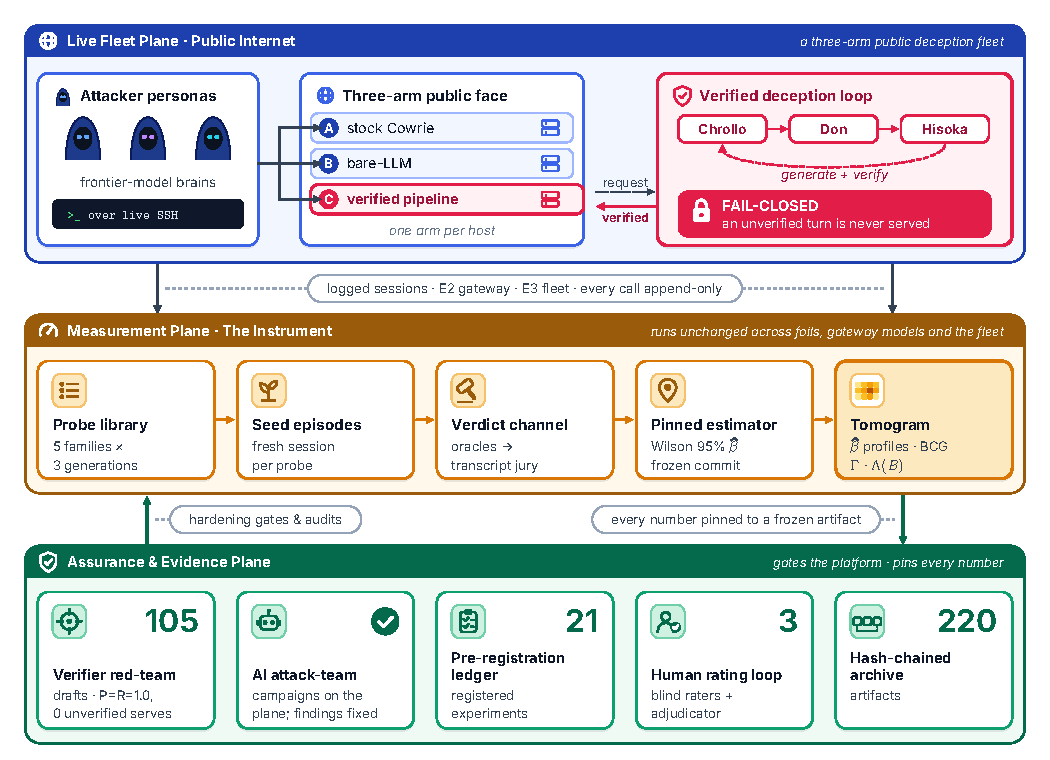
\includegraphics[width=\columnwidth]{anthro/fig3_platform.pdf}
\Description{A layered block diagram of the belief-tomography platform: a
three-arm public deception fleet behind one SSH face with a fail-closed
verified loop, the instrument layer (probe library, verdicts, frozen
estimator) running unchanged across foils, gateway models, and the fleet,
and an assurance--evidence layer gating the platform and pinning reported
numbers.}
\caption{The belief-tomography platform: a three-arm public deception fleet
whose verified loop fails closed; the instrument of
Section~\ref{sec:library} running unchanged across foils, gateway models,
and the fleet; and the assurance--evidence layer that gates the platform and
pins every reported number.}
\label{fig:platform}
\end{figure}

\paragraph{Adversarial assurance and evidence plane}
The platform's own defenses are measured like everything else. Labeled
adversarial drafts run through the real fiction-consistency verifier, and
in the retained serve logs every delivered record carries a passed
verifier check (no unverified serves); the earlier draft's specific
``105 cases, precision 1.0/recall 1.0'' calibration figure is withdrawn
as not reconstructible from the deposit. The
model-visible leakage audit covers the four completed field panels
(1{,}200 sessions, 1{,}600 turns; Section~\ref{sec:e2}); and every number
in this paper is
pinned by the claims--evidence ledger and its SHA-256 artifact manifest
(\texttt{CLAIMS\_EVIDENCE\_LEDGER.md} and
\texttt{ARTIFACT\_MANIFEST.sha256}, Data Availability), which hash the
registration and result artifacts as frozen---including the post-hoc
registration-file edits disclosed in Section~\ref{sec:limits}.
The decision layers and their gate studies (the Laya strategy selector,
held out of the default deployment; the JEV evidence judge, advisory-only)
and the claims--evidence ledger with its
manifest ship with the artifact package; the manifest's SHA-256
enumeration is the claim-to-artifact inventory (an earlier draft vouched a
separate ``codebase inventory,'' which has no on-disk artifact and is
withdrawn in favor of the manifest).



\end{document}
